% !TeX program = uplatex
% Compile: uplatex moduli_lecture_notes_rigorous.tex (2-3 times), then dvipdfmx moduli_lecture_notes_rigorous.dvi
% All figures are drawn with TikZ. No external images or bibliography files.
\documentclass[dvipdfmx,a4paper,11pt]{article}
\usepackage[uplatex]{otf}
\renewcommand{\kanjifamilydefault}{\gtdefault}
\usepackage{amsmath,amssymb,amsthm,mathrsfs,mathtools}
\usepackage[dvipdfmx]{graphicx}
\usepackage[dvipdfmx,dvipsnames]{xcolor}
\usepackage{tikz,tikz-cd}
\usetikzlibrary{arrows.meta,positioning,calc,decorations.markings}
\usepackage{enumitem,booktabs,longtable,array,setspace,etoolbox}
\usepackage[most]{tcolorbox}
\usepackage[top=25mm,bottom=28mm,left=25mm,right=25mm,headheight=14pt,headsep=8mm,footskip=15mm]{geometry}
\usepackage{fancyhdr,needspace}
\usepackage[dvipdfmx,colorlinks,linkcolor=blue!55!black,citecolor=blue!55!black,urlcolor=blue!55!black,unicode,hypertexnames=false]{hyperref}
\usepackage{pxjahyper}
\setstretch{1.13}
\setlength{\parindent}{0pt}
\setlength{\parskip}{5pt}
\setlength{\emergencystretch}{2em}
\setlist{itemsep=3pt,parsep=0pt,topsep=4pt}
\allowdisplaybreaks[2]
\setcounter{tocdepth}{2}
\preto\subsection{\Needspace{11\baselineskip}}
\renewcommand{\contentsname}{目次}
\renewcommand{\figurename}{図}
\clubpenalty=10000
\widowpenalty=10000
\displaywidowpenalty=10000
\renewcommand{\refname}{参考文献と原資料}
\renewcommand{\proofname}{証明}
\pagestyle{fancy}\fancyhf{}
\fancyhead[L]{\small リーマン面のモジュライ}
\fancyhead[R]{\small 定義・定理・証明}
\fancyfoot[C]{\thepage}
\renewcommand{\headrulewidth}{0.3pt}
\theoremstyle{definition}
\newtheorem{thm}{定理}[section]
\newtheorem{prop}[thm]{命題}
\newtheorem{lem}[thm]{補題}
\newtheorem{cor}[thm]{系}
\newtheorem{dfn}[thm]{定義}
\newtheorem{exa}[thm]{例}
\newtheorem{rem}[thm]{注意}
\newtheorem{ques}{確認問題}[section]
\tcbset{mybox/.style={colback=white,colframe=green!35!black,boxrule=.6pt,arc=1mm,breakable=false,before skip=8pt,after skip=8pt,left=7pt,right=7pt,top=5pt,bottom=5pt}}
\AtBeginEnvironment{thm}{\begin{tcolorbox}[mybox]}\AtEndEnvironment{thm}{\end{tcolorbox}}
\AtBeginEnvironment{prop}{\begin{tcolorbox}[mybox]}\AtEndEnvironment{prop}{\end{tcolorbox}}
\AtBeginEnvironment{dfn}{\begin{tcolorbox}[mybox]}\AtEndEnvironment{dfn}{\end{tcolorbox}}
\newenvironment{aim}{\begin{tcolorbox}[mybox,colback=green!3,title=この章で考えること,fonttitle=\bfseries]}{\end{tcolorbox}}
\newcommand{\C}{\mathbb C}\newcommand{\R}{\mathbb R}\newcommand{\Z}{\mathbb Z}\newcommand{\Q}{\mathbb Q}
\newcommand{\PP}{\mathbb P}\newcommand{\HH}{\mathbb H}
\newcommand{\OO}{\mathcal O}\newcommand{\MM}{\mathcal M}\newcommand{\TT}{\mathcal T}
\newcommand{\LL}{\mathcal L}\newcommand{\EE}{\mathbb E}
\DeclareMathOperator{\Aut}{Aut}\DeclareMathOperator{\Pic}{Pic}\DeclareMathOperator{\Hom}{Hom}
\DeclareMathOperator{\Spec}{Spec}\DeclareMathOperator{\Proj}{Proj}\DeclareMathOperator{\GL}{GL}
\DeclareMathOperator{\SL}{SL}\DeclareMathOperator{\PGL}{PGL}\DeclareMathOperator{\PSL}{PSL}
\DeclareMathOperator{\Sp}{Sp}\DeclareMathOperator{\Sym}{Sym}\DeclareMathOperator{\Ext}{Ext}
\DeclareMathOperator{\Res}{Res}\DeclareMathOperator{\Isom}{Isom}\DeclareMathOperator{\Diff}{Diff}
\DeclareMathOperator{\Hilb}{Hilb}\DeclareMathOperator{\rank}{rank}\DeclareMathOperator{\im}{im}
\newcommand{\inputtheorem}{\textbf{ここでは証明せず用いる定理。}}

\newcommand{\A}{\mathbb A}
\newcommand{\kk}{\mathbb C}
\newcommand{\Art}{\mathsf{Art}_{\C}}
\newcommand{\Def}{\operatorname{Def}}
\newcommand{\id}{\operatorname{id}}
\newcommand{\cM}{\overline{\mathcal M}}
\newcommand{\cH}{\overline H}
\newcommand{\eps}{\varepsilon}
\DeclareMathOperator{\coker}{coker}
\DeclareMathOperator{\End}{End}
\DeclareMathOperator{\Der}{Der}
\DeclareMathOperator{\Stab}{Stab}
\DeclareMathOperator{\Gal}{Gal}
\DeclareMathOperator{\tr}{tr}
\DeclareMathOperator{\codim}{codim}
\newenvironment{external}[1]{\Needspace{7\baselineskip}\refstepcounter{thm}\begin{tcolorbox}[mybox,colback=blue!2,colframe=blue!40!black]\textbf{引用定理 \thethm（#1）}\par}{\end{tcolorbox}}
\newenvironment{point}{\begin{tcolorbox}[mybox,colback=green!2]\textbf{論理上の確認}\par}{\end{tcolorbox}}
\title{リーマン面と代数曲線のモジュライ\\[4mm]\large 定義・定理・証明を中心とする大学院講義ノート}
\author{岩井雅崇氏の授業資料をもとにした再構成稿\\\small 主資料：R. Hain / D. Edidin}
\date{2026年9月24日：証明・具体例を増補した改訂版}
\hypersetup{pdftitle={リーマン面と代数曲線のモジュライ：定義・定理・証明}}
\begin{document}
\maketitle
\section*{本ノートの目的と読み方}
リーマン面の分類では、個々の曲線の同型類を調べるだけでなく、それらが族の中でどのように動くかを考える。
本ノートでは、具体的な分類から始め、変形、Teichmüller 空間、スタックを通して、曲線のモジュライ空間の構成へ進む。
さらに、その位相と Hodge 線束を調べる。元の和文資料の解析的な部分は Hain \cite{Hain}、代数的な部分は Edidin \cite{Edidin} に対応する。
逐語訳ではなく、定義の補足、証明の展開、規約の統一を行った講義用の再構成である。

前提は『リーマン面・代数曲線論』2026年9月21日版である。
特に、因子と線束、層と Čech コホモロジー、Riemann--Roch、Serre 双対性、Hodge 分解、射影埋め込み、標準写像、曲線の自己同型群を使用する。
本ノートに現れるスキーム・降下・変形理論の新しい用語は、その使用前に定義する。
ただし、一般の代数幾何学や変形理論を一冊分展開することはしない。必要な存在定理は正確な形で独立に記す。

\textbf{証明の扱い。}
番号を付けた定理・命題には、本文の証明、または証明を外部に委ねることを示す青枠と出典を付ける。
「引用する定理」の枠は証明ではない。その後の「証明」では、その入力から導く結果を証明する。
補足的な説明には、証明の代わりとなる論拠を隠さない。
演習のうち本文に必要な事実は、演習の解答に依存させず本文で示す。

\textbf{証明を読むために。}
長い証明では、最初に何を構成するかを述べ、構成・選択への依存・逆の対応を分けて確認する。
「同型類が対応する」と「対象とすべての同型射が対応する」の違いは、主束と降下の具体例で繰り返し扱う。
図は写像の関係や退化の局所模型を示すものであり、図だけで存在や一意性を結論しない。
最初の通読では具体例を計算してから証明に戻り、二度目には各段階で使った仮定を確認するとよい。

\textbf{基礎体と圏。}
基本の体は $\C$ である。解析的な族では複素解析空間、代数的な族では局所 Noether 的な $\C$-スキームを基底とする。
無限小変形では非被約な Artin スキームも許す。
すべての曲線は、断らない限り連結・コンパクトなリーマン面、または射影的な代数曲線である。
滑らかな射影代数曲線とコンパクトリーマン面の同値は既習の代数化定理による。
しかし、\emph{族の比較}は点ごとの代数化だけでは済まない。両モジュライの比較は第\ref{sec:compact}節で独立の定理として用いる。

\clearpage
\section*{記号と講義の見取り図}
\textbf{主要な記号。}
\[
\begin{array}{c|l}
M_{g,n}&\text{同型類の集合、構成後はその粗モジュライ空間}\\
\MM_{g,n}&\text{族と同型を記録するモジュライスタック}\\
\MM_{g,n}^{\rm an}&\text{解析的なモジュライスタック}\\
\TT_{g,n}&\text{マーキング付き曲線の Teichmüller 空間}\\
\Gamma_{g,n}&\text{向きを保ち、各標点を固定する写像類群}\\
\cM_g,\ \overline M_g&\text{安定曲線のスタックとその粗モジュライ空間}.
\end{array}
\]
$n=0$ のとき添字 $n$ を省略する。楕円曲線については常に原点を指定し、$\MM_{1,1}$ と書く。
Hain の $\mathcal M_1$ はこの意味で読み替える。
全体として安定範囲 $2g-2+n>0$ を重視する。
GIT の構成は Edidin の数値条件に合わせて $g\ge3$ で詳述し、$g=2$ を含む存在定理は適用範囲を明記して引用する。

\begin{center}
\begin{tikzpicture}[>=Stealth,box/.style={draw=green!40!black,rounded corners,align=center,text width=5.1cm,inner sep=7pt},node distance=10mm]
\node[box,text width=11.5cm] (family) {曲線の族と同型\\種数 $0,1$ の具体例・無限小変形};
\node[box] (teich) at (-3.2,-2.0) {解析的な構成\\Teichmüller 空間・写像類群};
\node[box] (stable) at (3.2,-2.0) {代数的な構成\\安定曲線・多重標準埋め込み};
\node[box,below=of teich] (orb) {オービフォールド $[\TT_g/\Gamma_g]$\\レベル構造・群コホモロジー};
\node[box,below=of stable] (git) {商スタック $[\overline H/\PGL]$\\GIT・粗モジュライ空間};
\node[box,text width=11.5cm] (last) at (0,-6.8) {解析的構成と代数的構成の比較\\Hodge 束・Picard 群};
\draw[->] (family.south)--++(0,-.3)-|(teich.north);
\draw[->] (family.south)--++(0,-.3)-|(stable.north);
\draw[->] (teich)--(orb);\draw[->] (stable)--(git);
\draw[->] (orb.south)--++(0,-.3)-|(last.north);
\draw[->] (git.south)--++(0,-.3)-|(last.north);
\end{tikzpicture}
\end{center}

\textbf{読む順序。}
第\ref{sec:families}--\ref{sec:period}節が解析的な道筋、第\ref{sec:schemes}--\ref{sec:compact}節が代数的な道筋である。
両者の接点は「自己同型を保った局所変形の商」にある。
最後の第\ref{sec:mcg}--\ref{sec:pic}節で、Hain の写像類群・Picard 群の議論をつなぐ。
末尾には解答付き演習、引用結果の依存表、原著の規約・誤植についての注記を置いた。
\clearpage
\tableofcontents
\clearpage

\section{分類問題と曲線の族}\label{sec:families}
\begin{aim}
同型類の集合を作ることと、族を分類する空間を作ることを区別する。以後の普遍性の定義で、何が一意でなければならないかを明確にする。
\end{aim}
\subsection{点付き曲線とその同型}
\begin{dfn}
種数 $g$ の $n$ 点付き滑らかな曲線とは、滑らかな曲線 $C$ と相異なる順序付きの点 $p_1,\ldots,p_n$ の組である。
同型 $f:(C;p_i)\to(C';p_i')$ は $f(p_i)=p_i'$ を満たす双正則写像である。
その同型類の集合を $M_{g,n}$ とする。$n=0$ の場合は $M_g$ と書く。
\end{dfn}
点の順序は定義の一部である。点の集合を保つ自己同型群と、各点を固定する自己同型群は異なる。
\begin{prop}\label{prop:finiteaut}
滑らかな点付き曲線の自己同型群 $\Aut(C;p_i)$ が有限であるための必要十分条件は $2g-2+n>0$ である。
\end{prop}
\begin{proof}
$g=0$ では $C\simeq\PP^1$ である。三点を固定する一次分数変換は恒等写像である。
一点以下なら affine 変換の無限部分群、二点なら $z\mapsto az$ の無限部分群が残る。
$g=1$ で標点がなければ平行移動が残る。一点を原点にすると自己同型群は有限である（既習ノートの種数 $1$ の自己同型の定理）。
$g\ge2$ では $\Aut(C)$ 自体が有限であり、標点を固定する群はその部分群である。
\end{proof}
\subsection{族、引き戻し、同型}
\begin{dfn}[解析的な滑らかな族]\label{def:family}
複素解析空間 $B$ 上の種数 $g$ の滑らかな曲線の族は、proper かつ smooth な正則射 $\pi:X\to B$ で、各ファイバーが連結な種数 $g$ の曲線となるものである。
$n$ 点付き族には、互いに交わらない正則切断 $s_i:B\to X$ を付ける。
$B$ が多様体なら smooth は $X$ が多様体で $\pi$ が劣沈であることと同値である。
一般の解析空間では、各点の近くで $B\times\C$ への開埋め込みを通じて射影に一致する、という相対的な意味を用いる。
\end{dfn}
proper とはコンパクト集合の逆像がコンパクトであることをいう。滑らかさだけではファイバーの穴が無限遠へ逃げる可能性を排除できない。
非被約基底まで扱う理由は、第\ref{sec:def}節で一次の変化を記録するためである。

\begin{dfn}[族の射と基底変換]
同じ $B$ 上の二つの族の同型は、$B$ 上の同型 $F:X\to X'$ で $F\circ s_i=s_i'$ を満たすものである。
射 $f:B'\to B$ に沿う引き戻しは
\[
X_{B'}=B'\times_B X\longrightarrow B',\qquad
s_{i,B'}(b')=(b',s_i(f(b')))
\]
である。異なる基底上の族の射には、次の正方形が Cartesian であることを要求する。
\[
\begin{tikzcd}
X'\ar[r]\ar[d]&X\ar[d,"\pi"]\\
B'\ar[r,"f"]&B.
\end{tikzcd}
\]
すなわち $X'\to B'\times_BX$ が標点を保つ同型でなければならない。
\end{dfn}
単に可換な正方形では、ファイバー上の任意の正則写像まで許してしまう。モジュライではファイバーの同型を記録したいので Cartesian 条件が必要である。

\begin{dfn}[集合値モジュライ関手]
$F_{g,n}(B)$ を $B$ 上の $n$ 点付き種数 $g$ の族の同型類の集合とする。
引き戻しによって反変関手 $F_{g,n}$ が得られる。
$F_{g,n}$ を表現する空間 $M$ とは、すべての基底について自然な全単射
\[
\Hom(B,M)\xrightarrow{\sim}F_{g,n}(B)
\]
を与える空間である。$\id_M$ に対応する族を普遍族という。このような $M$ を fine moduli space と呼ぶ。
\end{dfn}
「自然」とは、$B'\to B$ による写像の合成が、族の引き戻しに対応することである。
この定義は\emph{族の同型類}についての普遍性である。同型そのものの一意性まで述べるには、後で亜群を使う。

\begin{dfn}[粗モジュライ空間：集合値関手による形]\label{def:coarsefunctor}
$F$ の粗モジュライ空間は、空間 $M$ と自然変換 $\eta:F\to\Hom(-,M)$ で、次を満たすものである。
\begin{enumerate}
\item 幾何学的な点上では同型類と点を一対一に対応させる。解析的には $B=\{\mathrm{pt}\}$、代数的には任意の代数閉拡大体の点で要求する。
\item 任意の空間 $Y$ と自然変換 $\theta:F\to\Hom(-,Y)$ に対し、一意な射 $u:M\to Y$ が存在し、$\theta=u\circ\eta$ となる。
\end{enumerate}
\end{dfn}
粗モジュライ写像 $B\to M$ は族から得られる。しかし、任意の $B\to M$ に族が付随することも、付随する族が一意であることも、この定義は要求しない。
第\ref{sec:stacks}節ではスタックから代数空間への普遍性として定義し直す。

\subsection{一定の同型類をもつ、非自明な族}
\begin{prop}[ねじれた楕円曲線族]\label{prop:twist}
原点付き楕円曲線 $E$ と $B'=\C^*$ をとる。位数 $2$ の群が
\[
(x,u)\longmapsto(-x,-u)
\]
で $E\times B'$ に作用する。商 $X=(E\times B')/\{\pm1\}$ は $B=\C^*$ 上の滑らかな原点付き楕円曲線族である。射は $t=u^2$ で与える。
各ファイバーは $E$ と同型であるが、この族は $E\times B$ と同型ではない。
\end{prop}
\begin{proof}
\textbf{方針。} 局所的には積であることを確認し、大域的に一周したときの「戻り方」が積族と異なることを示す。

\textbf{1. 局所的な自明化を作る。}
$B$ の小さな単連結開集合 $V$ では、$t$ の正則な平方根 $r(t)$ を選べる。
\[
E\times V\longrightarrow X|_V,\qquad (x,t)\longmapsto[x,r(t)]
\]
は同型である。実際、$u^2=t$ なら $u=r(t)$ または $-r(t)$ であり、後者の代表元は $[x,-r(t)]=[-x,r(t)]$ と書き直せる。
こうして逆写像も得られる。従って射は局所的に射影 $E\times V\to V$ に一致し、proper かつ smooth である。
平方根の符号を変えても $[0,r(t)]=[0,-r(t)]$ なので原点切断も貼り合う。

\textbf{2. 閉じた道に沿ってファイバーを運ぶ。}
$t(s)=e^{2\pi i s}$、$0\le s\le1$ を考える。その平方根を $u(0)=1$ から連続的に追うと $u(s)=e^{\pi i s}$、従って $u(1)=-1$ となる。
$x\in E$ を固定して $[x,u(s)]$ を追うと、終点は
\[
[x,-1]=[-x,1]
\]
である。最初のファイバーを $x\mapsto[x,1]$ で $E$ と同定しておくと、一周後の写像は $x\mapsto-x$ になる。
これがこの道のモノドロミーである。

\textbf{3. 積族との違いを不変量で検出する。}
$H_1(E,\Z)\simeq\Z^2$ の二つの基本閉曲線は $x\mapsto-x$ によってともに向きを反転する。
従ってホモロジーのモノドロミーは $-I$ であり、双対な $R^1\pi_*\Z$ でも $-I$ である。
積族なら $x$ を一定に運べるからモノドロミーは $I$ となる。
族の同型が存在すれば、基準ファイバー上の同型 $A$ により両者は共役になるはずだが、$AIA^{-1}=I\neq-I$ である。
従って族は同型ではない。
\end{proof}
\par\medskip
\noindent\begin{minipage}{\linewidth}
\begin{center}
\begin{tikzpicture}[>=Stealth,node distance=13mm]
\node (t0) at (0,0) {$t=1$}; \node (t1) at (5,0) {$t=1$};
\node (u0) at (0,1) {$u=1$}; \node (u1) at (5,1) {$u=-1$};
\draw[->] (t0)--node[below]{底で一周：$e^{2\pi i s}$}(t1);
\draw[->] (u0)--node[above]{持ち上げ：$e^{\pi i s}$}(u1);
\draw[->] (u0)--(t0); \draw[->] (u1)--(t1);
\node[align=center] at (2.5,-1.1) {同じ底の点に戻っても、曲線の同定は $x\mapsto-x$};
\end{tikzpicture}
\end{center}
\end{minipage}\par\medskip

\begin{cor}
解析的な楕円曲線の集合値関手 $F_{1,1}$ を表現する複素解析空間は存在しない。
\end{cor}
\begin{proof}
表現空間 $M$ とその普遍族 $\mathscr U\to M$ があると仮定する。
命題\ref{prop:twist}の族に対応する分類写像を $f:B\to M$ とする。
一点 $b\in B$ への引き戻しと分類の自然性により、$f(b)$ は $X_b$ の同型類を表す。
すべての $X_b$ は $E$ と同型なので、$f$ の像は一つの点 $m=[E]$ に含まれる。

ここで $B=\C^*$ は被約である。
$M$ を点 $m$ の近くで局所的に複素 Euclid 空間へ埋め込み、各座標関数を $B$ へ引き戻すと、値はすべての点で一定である。
被約な解析空間上の正則関数は点での値により決まるので、これらは関数として一定である。
従って $f$ は射として $B\to\{m\}\to M$ を経由する。
その普遍族の引き戻しは $B\times\mathscr U_m\simeq B\times E$ となる。
表現性により $X\simeq f^*\mathscr U$ でなければならないが、これはねじれた族が積族でないことに矛盾する。
\end{proof}
この証明では「すべてのファイバーが同型」から「族が自明」を結論していない。
逆に、その二つが異なることをモノドロミーで検出した。

\par\bigskip\Needspace{.70\textheight}
\section{種数ゼロ：複比から普遍族まで}\label{sec:g0}
\begin{aim}
一つの分類問題について、同型類の分類、空間の構造、任意の族に対する普遍性までを順に証明する。
\end{aim}
\subsection{三点の正規化}
\begin{lem}\label{lem:normalize}
相異なる $a,b,c\in\PP^1$ をそれぞれ $0,1,\infty$ に送る一次分数変換は一意である。
三点が有限なら、その写像は
\[
N_{a,b,c}(z)=\frac{(z-a)(b-c)}{(z-c)(b-a)}
\]
で与えられる。
\end{lem}
\begin{proof}
まず $a,b,c$ が有限な場合を考える。
$a,b,c$ は相異なるので式の定数因子 $(b-c)/(b-a)$ は非零であり、分子と分母の零点も異なる。
従って $N_{a,b,c}$ は次数一の分数変換である。
$z=a$ で値は $0$、$z=b$ で値は $1$、$z=c$ では極をもつので値は $\infty$ となる。
三点のいずれかが $\infty$ の場合には、三点の外に一点を選んでそれを無限遠とする座標を先に取り、この式を使えばよい。
例えば $c=\infty$ なら直接 $N(z)=(z-a)/(b-a)$ と書ける。

一意性を示すため、二つの候補を $N,N'$ とする。
$N'\circ N^{-1}$ は $0,1,\infty$ を固定する。
一次分数変換 $(Az+B)/(Cz+D)$ が $0,\infty$ を固定する条件は $B=C=0$ なので、$z\mapsto uz$ の形になる。
さらに $1$ を固定すれば $u=1$ となり、$N'\circ N^{-1}=\id$、従って $N'=N$ である。
\end{proof}
\begin{thm}[点付き種数ゼロ曲線の分類]\label{thm:g0}
$n\ge3$ とする。$M_{0,n}$ は次の滑らかな affine 多様体と同一視される。
\[
U_n=\{(t_4,\ldots,t_n)\in\C^{n-3}\mid
 t_i\neq0,1,\quad t_i\neq t_j\ (i\neq j)\}.
\]
特に $M_{0,3}$ は一点、$M_{0,4}=\PP^1\setminus\{0,1,\infty\}$ である。
\end{thm}
\begin{proof}
$C\simeq\PP^1$ を選び、最初の三点を補題で正規化する。残りの点の像が $t_i$ を与える。
最初の同型の選択を変えても、正規化の一意性から結果は変わらない。
同型な配置も同じ $t_i$ を与える。逆に $t_i$ が一致すれば、二つの正規化写像の合成が点付き同型を与える。
任意の $U_n$ の点は $(\PP^1;0,1,\infty,t_4,\ldots,t_n)$ から生じるので全単射である。

$U_n$ は多項式
$D=\prod_{i=4}^nt_i(t_i-1)\prod_{4\le i<j\le n}(t_i-t_j)$
の非消滅集合である。従って $U_n=\Spec\C[t_4,\ldots,t_n,D^{-1}]$ は affine であり、$\C^{n-3}$ の開集合だから滑らかで次元 $n-3$ である。空積は $1$ とする。
\end{proof}
ここまでは集合上の分類と、その集合に入れる自然な空間構造を示した。次に、正則に動く族が正則な $t_i$ を与えることを証明する。

\subsection{族の正規化を保証する準備}
\begin{external}{Grauert の基底変換定理の使用形}\label{input:grauert}
$\pi:X\to B$ を proper な解析的射、$L$ を $B$ 上平坦な連接層とする。すべてのファイバーで $H^1(X_b,L_b)=0$、$h^0(X_b,L_b)=r$ と仮定する。
このとき $\pi_*L$ は階数 $r$ の局所自由層であり、その形成は任意の解析的基底変換と可換である。
以下では $\pi$ は曲線の滑らかな族、$L$ は線束の場合に使う。
出典は \cite{Grauert} の基底変換定理。代数的な対応物は第\ref{sec:schemes}節に記す。
\end{external}
\begin{lem}[三切断をもつ族の自明化]\label{lem:threefamily}
種数 $0$ の滑らかな族 $X\to B$ が互いに交わらない三切断 $s_1,s_2,s_3$ をもつとき、これらを $0,1,\infty$ に送る $B$ 上の同型 $X\simeq\PP^1\times B$ が一意に存在する。
\end{lem}
\begin{proof}
\textbf{方針。} 各ファイバーを別々に $\PP^1$ と同定するだけでは、同定が正則に変化するとはいえない。
まず二つの切断の基底を局所的に正則に選び、そこから射影座標を作る。

\textbf{1. 次数一の線束から射影座標を作る。}
切断 $s_3$ の像は相対 Cartier 因子なので $L=\OO_X(s_3)$ を作れる。
各ファイバー $X_b\simeq\PP^1$ では $L_b\simeq\OO_{\PP^1}(1)$ であり、$h^0(L_b)=2$、$h^1(L_b)=0$ である。
引用定理\ref{input:grauert}により $V=\pi_*L$ は階数二のベクトル束で、$V\otimes\C(b)\simeq H^0(X_b,L_b)$ となる。
従って $V$ の局所基底は、各ファイバーの完全線形系の基底を与える。

評価写像 $\pi^*V\to L$ を考える。余核を $Q$ とすると、ファイバー上の $\OO(1)$ は大域生成だから $Q\otimes\C(b)=0$ である。
各点の局所環で Nakayama の補題を適用すると $Q=0$ を得る。
ここで用いた補題は「有限生成加群 $M$ が $M/JM=0$ を満たし、$J$ が極大イデアルに含まれれば $M=0$」という形である。
こうして射 $j:X\to\PP_B(V^\vee)$ が定まる。

\textbf{2. ファイバー上の埋め込みを族の埋め込みにする。}
$j_b$ は $\OO(1)$ の完全系による $\PP^1\to\PP^1$、従って同型である。
ここで相対 very ample 判定を使う：proper flat な族の線束が各ファイバーで very ample で、その切断の直像が基底変換と可換なら、評価写像は相対閉埋め込みを与える。
これは基底変換定理の標準的な相対埋め込みの形であり、代数的な版は引用定理\ref{input:basechange}に記す。
従って $j$ は閉埋め込みである。
そのイデアル層を $J$ とすると、商である $\OO_X$ は $B$ 上 flat なので、ファイバーへの制限でもイデアルの完全系列は左側まで完全である。
$j_b$ が同型であることから $J\otimes\C(b)=0$、再び Nakayama により $J=0$ となる。よって $j$ 自身が同型である。

\textbf{3. 三切断を使って局所座標を一意にそろえる。}
$V$ の局所自明化により $X|_W\simeq\PP^1\times W$ を得る。
必要なら $W$ を小さくし、三切断を同じ affine 座標で $a(b),b(b),c(b)$ と書く。
補題\ref{lem:normalize}の分数式の差 $a-b,b-c,c-a$ は可逆なので、正規化は基底に正則に依存する。

重なり上で二つの正規化を比較する。$0,\infty$ を固定する射影行列は局所的に対角行列で、$1$ も固定すれば二つの対角成分は等しい。
従って $\PGL_2$ の元として恒等元である。この計算は非被約基底でも有効である。
よって正規化は重なりで一致して大域的に貼り合い、同じ議論で一意性も従う。
\end{proof}
\begin{thm}[普遍族]\label{thm:univg0}
$\PP^1\times U_n\to U_n$ に切断 $0,1,\infty,t_4,\ldots,t_n$ を付けた族は、$n$ 点付き種数 $0$ 曲線の解析的な普遍族である。
任意の族は一意な正則写像 $B\to U_n$ による引き戻しであり、標点を保つ引き戻し同型も一意である。
\end{thm}
\begin{proof}
$\pi:X\to B$ と $n$ 本の切断 $s_i$ を与える。
前の補題により、最初の三切断を $0,1,\infty$ に送る一意な同型
$F:X\xrightarrow{\sim}\PP^1\times B$ がある。
$F\circ s_i$ の第一成分を $t_i:B\to\PP^1$ と置く。
$i\ge4$ では $s_i$ が $s_3$ と交わらないため $t_i$ は $\infty$ を避け、実際に $\C$ 値の正則関数となる。
他の切断との非交叉から $t_i\neq0,1$、$t_i\neq t_j$ が成り立つので
\[
t=(t_4,\ldots,t_n):B\longrightarrow U_n
\]
が定まる。
普遍候補の $t$ による引き戻しは、積族に切断 $0,1,\infty,t_4(b),\ldots,t_n(b)$ を付けたものであり、$F$ はもとの点付き族との同型を与える。

別の分類写像 $t'$ と引き戻し同型があれば、それも最初の三切断を同じ位置へ送るので、正規化の一意性から同型は $F$ と一致する。
すると残る切断の第一成分も一致し、$t'=t$ である。
構成を基底変換しても同じ三点の正規化を行うので対応は自然であり、関手を表現する普遍性を得る。
\end{proof}
\begin{exa}[分類写像を実際に書く]
$B=\C\setminus\{0,1\}$ 上の積族に、切断 $0,2,\infty,2b$ を付ける。
最初の三点の正規化は $z\mapsto z/2$ なので分類写像は $b\mapsto b$ である。
第四切断を $2b^2$ に替えると、基底を $\C\setminus\{0,1,-1\}$ に制限する必要があり、分類写像は $b\mapsto b^2$ となる。
$\PP^1\times B$ という全空間だけでは、点付き族の分類写像は決まらない。
切断も含めたデータが必要である。
\end{exa}

\subsection{複比と順序を忘れる操作}
$n=4$ の座標は
\[
t=\frac{(p_4-p_1)(p_2-p_3)}{(p_4-p_3)(p_2-p_1)}
\]
である。点の順序を変えると
\[
t,\quad1-t,\quad t^{-1},\quad(1-t)^{-1},\quad\frac{t-1}{t},\quad\frac t{t-1}
\]
が現れる。例えば第一点と第二点の交換は $z\mapsto1-z$ によって $t\mapsto1-t$ を与える。
順序付き配置の自己同型は自明だが、順序を忘れた配置では有限な対称性が復活する。
$t=-1$ では上の六つの値がすべて異なるわけではない。この現象を後の商空間の分岐と比較するとよい。

\begin{exa}[超楕円曲線のパラメータ]
種数 $g\ge2$ の超楕円曲線は、$\PP^1$ 上の相異なる $2g+2$ 点を分岐点にもつ二重被覆である。
既習の超楕円写像の一意性と二重被覆の分類から、その同型類は順序を忘れた分岐点配置で決まる。
従って超楕円曲線の同型類の集合は $M_{0,2g+2}/\mathfrak S_{2g+2}$ で記述され、有限商の次元は $2g-1$ である。
ただし、分岐点配置のスタックと超楕円曲線のスタックはそのまま同じではない。曲線側には超楕円対合が常に残る。
\end{exa}

\par\bigskip\Needspace{.70\textheight}
\section{楕円曲線：格子、周期、群作用}\label{sec:elliptic}
\begin{aim}
上半平面の点が何を分類するかを明確にし、$\SL_2(\Z)$ の作用と族の周期写像を導く。
\end{aim}
\subsection{原点を固定する意味}
\begin{dfn}
楕円曲線は、種数 $1$ の曲線 $E$ と一点 $0\in E$ の組である。同型は原点を保つものとする。
$\tau\in\HH$ に対し、$\Lambda_\tau=\Z+\Z\tau$、$E_\tau=\C/\Lambda_\tau$ と置く。
\end{dfn}
既習ノートの積分による一意化から、任意の楕円曲線はある $E_\tau$ に同型である。
原点を忘れると、すべての平行移動が自己同型となる。以下の有限群の議論では原点を忘れてはいけない。

\begin{lem}[複素トーラス間の写像]\label{lem:torusmap}
正則写像 $f:\C/\Lambda\to\C/\Lambda'$ は $z\mapsto az+b$ で誘導される。ただし $a\Lambda\subset\Lambda'$ である。
原点を保つ同型なら $b=0$ と選べ、$a\neq0$、$a\Lambda=\Lambda'$ となる。
\end{lem}
\begin{proof}
\textbf{1. 商の上の写像を平面へ持ち上げる。}
商写像を $p:\C\to\C/\Lambda$、$p':\C\to\C/\Lambda'$ と書く。
$\C$ は単連結なので、$f\circ p$ はある $F:\C\to\C$ に持ち上がり、$p'F=fp$ を満たす。
被覆写像 $p'$ は局所双正則だから $F$ は整関数である。

\textbf{2. 微分すると格子による曖昧さが消える。}
$\lambda\in\Lambda$ に対して $p(z+\lambda)=p(z)$ なので、
$F(z+\lambda)-F(z)\in\Lambda'$ である。
左辺は $z$ の連続関数、右辺は離散集合であり、$\C$ は連結だから、この差は $z$ に依存しない。
従って $F'(z+\lambda)=F'(z)$ となる。
$F'$ は閉基本平行四辺形上で有界で、平面上の任意の点は格子移動によってその中に入る。
よって $F'$ は平面全体で有界である。Liouville の定理を $F'$ に適用して $F'=a$、従って $F(z)=az+b$ を得る。
また $F(z+\lambda)-F(z)=a\lambda\in\Lambda'$ より $a\Lambda\subset\Lambda'$ である。

\textbf{3. 同型である条件を確かめる。}
原点を保つなら $F(0)\in\Lambda'$ なので、持ち上げからこの格子元を引いて $b=0$ とできる。
$f$ が同型なら、逆写像も原点を保つ $z\mapsto a'z$ で誘導される。
合成の持ち上げは原点を固定する恒等写像だから $a'a=1$ である。
$a\Lambda\subset\Lambda'$ と $a'\Lambda'\subset\Lambda$ を合わせると $a\Lambda=\Lambda'$ を得る。
逆にこの等式が成り立てば、$z\mapsto a^{-1}z$ が商上の逆写像を与える。
\end{proof}

\begin{thm}[楕円曲線の同型条件]\label{thm:elliso}
$E_\tau\simeq E_{\tau'}$ であることと、ある
$\gamma=\left(\begin{smallmatrix}a&b\\c&d\end{smallmatrix}\right)\in\SL_2(\Z)$ によって
\[
\tau'=\gamma\tau:=\frac{a\tau+b}{c\tau+d}
\]
となることは同値である。このとき $z\mapsto z/(c\tau+d)$ が同型を与える。
\end{thm}
\begin{proof}
\textbf{分数線形変換から同型を作る。}
$ad-bc=1$ なら、$\Lambda_\tau$ の二つの元
$c\tau+d$ と $a\tau+b$ は整数基底である。実際、基底 $(1,\tau)$ に関する係数行列
$\left(\begin{smallmatrix}d&b\\c&a\end{smallmatrix}\right)$ の行列式は $1$ で、逆行列も整数行列である。
全体を $c\tau+d$ で割ると基底 $1,\gamma\tau$ になるから
\[
(c\tau+d)^{-1}\Lambda_\tau=\Lambda_{\gamma\tau}.
\]
従って前の補題により、指定された写像が同型となる。

\textbf{同型から整数行列を取り出す。}
逆に同型が $z\mapsto az$ で与えられたとする。ここだけ定数を $v$ と書き替え、$v\Lambda_\tau=\Lambda_{\tau'}$ とする。
$v^{-1}$ と $v^{-1}\tau'$ は $\Lambda_\tau$ の基底だから、整数 $A,B,C,D$ によって
\[
v^{-1}=C\tau+D,\qquad v^{-1}\tau'=A\tau+B
\]
と書ける。基底変換の行列式は $\pm1$ である。
複素数倍は実平面の向きを保ち、$(1,\tau)$、$(1,\tau')$ はともに正の向きなので $AD-BC=1$ となる。
二つの等式を割ると $\tau'=(A\tau+B)/(C\tau+D)$ を得る。
最後に直接計算で
\[
\Im\frac{A\tau+B}{C\tau+D}
=\frac{(AD-BC)\Im\tau}{|C\tau+D|^2}>0
\]
となり、作用が上半平面を保つことも確認できる。
\end{proof}
\begin{exa}[同じトーラスを与える二つの格子基底]
$T=\left(\begin{smallmatrix}1&1\\0&1\end{smallmatrix}\right)$ は $\tau\mapsto\tau+1$ を与える。
この場合 $\Z+\Z(\tau+1)=\Z+\Z\tau$ なので、曲線上の同型は恒等写像である。
一方 $S=\left(\begin{smallmatrix}0&-1\\1&0\end{smallmatrix}\right)$ では $\tau\mapsto-1/\tau$、同型は $z\mapsto z/\tau$ である。
$\tau=i$ では底の点は固定されるが、曲線上では $z\mapsto-iz$ という位数四の自己同型になる。
「底の点を固定する」と「曲線上で恒等である」は異なる。
\end{exa}

従って集合として $M_{1,1}=\SL_2(\Z)\backslash\HH$ である。
$-I$ は $\HH$ 上自明に作用するが、対応する楕円曲線の同型は $z\mapsto-z$ である。この違いは後で本質的になる。

\subsection{固定点群と局所的な商}
\begin{prop}\label{prop:ellaut}
$\Aut(E_\tau,0)$ は、一般の $\tau$ では $\mu_2$、$\tau=i$ の軌道上では $\mu_4$、$\rho=e^{2\pi i/3}$ の軌道上では $\mu_6$ である。
ここで $\mu_r=\{z\in\C^*\mid z^r=1\}$ とする。
\end{prop}
\begin{proof}
\textbf{1. 自己同型に現れる定数を制限する。}
前の補題から自己同型は $z\mapsto az$、$a\Lambda=\Lambda$ である。
複素数倍は実面積を $|a|^2$ 倍する。同じ格子の基本領域の面積を比較すると $|a|^2=1$ となる。
実線形変換 $z\mapsto az$ の固有値は $a,\bar a$ であり、格子基底では整数行列なので
\[
a+\bar a=2\Re a\in\{-2,-1,0,1,2\}.
\]
単位円上でこの五通りを解くと、$a=\pm1$、$\pm i$、または原始三乗根・六乗根である。

\textbf{2. 特別な回転を許す格子を決める。}
$i\Lambda=\Lambda$ なら $\Lambda$ は $\Z[i]$-加群である。
非零の $\lambda\in\Lambda$ を取り、$\lambda^{-1}\Lambda$ を考える。
その有理線形包は $i$ を含む二次元 $\Q$-空間なので $\Q(i)$ に一致する。
共通の整数分母を払えば $N\lambda^{-1}\Lambda\subset\Z[i]$ となり、これは非零イデアルである。
$\Z[i]$ は Euclid 環、従って単項イデアル整域なので、このイデアルは $\alpha\Z[i]$ の形である。
よって $\Lambda$ は $\Z[i]$ の複素数倍である。
三乗根・六乗根の場合も、$\Z[\rho]$ が Euclid 環であることを用いて同様に示せる。
ここで両環の Euclid 性は複素絶対値の二乗を用いる整数論の標準結果である。

\textbf{3. 群全体を読む。}
正方格子を保つ回転は $\pm1,\pm i$、六角格子を保つ回転は六乗根全体である。
それ以外の格子では第2段階に該当する回転は存在せず、常に存在する $\pm1$ だけが残る。
格子を定数倍してもトーラスの同型類は変わらないので、主張された三通りを得る。
\end{proof}
\begin{external}{上半平面の商の基本性質}
$\PSL_2(\Z)$ は $\HH$ に properly discontinuously に作用し、
\[
\{\tau\in\HH\mid |\Re\tau|\le1/2,\ |\tau|\ge1\}
\]
は境界の同一視を伴う基本領域である。
商は一意なリーマン面構造をもち、局所的には固定点群による円板の商で記述される。
出典：Hain \cite{Hain}, Theorem 2.20 とその前後。
\end{external}
有限巡回群が円板に $z\mapsto\zeta z$ で作用すると、商の座標は $w=z^r$ である。
従って商の点自体は滑らかでも、写像には分岐があり、元の固定点群の情報は失われる。

\par\medskip
\noindent\begin{minipage}{\linewidth}
\begin{center}
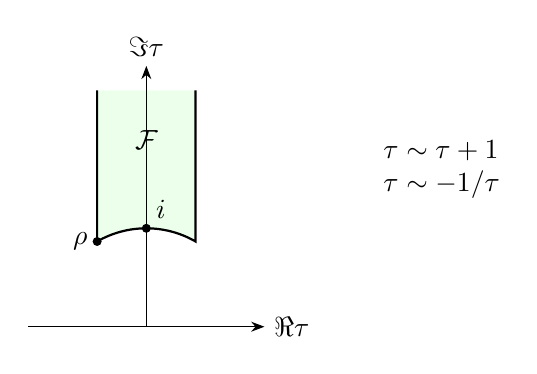
\begin{tikzpicture}[scale=1.25,>=Stealth]
\fill[green!8] (-.5,2.4)--(-.5,.866) arc(120:60:1)--(.5,2.4)--cycle;
\draw[->] (-1.2,0)--(1.2,0) node[right] {$\Re\tau$};
\draw[->] (0,0)--(0,2.65) node[above] {$\Im\tau$};
\draw[thick] (-.5,2.4)--(-.5,.866) arc(120:60:1)--(.5,2.4);
\fill (0,1) circle(1.3pt) node[above right] {$i$};
\fill (-.5,.866) circle(1.3pt) node[left] {$\rho$};
\node at (0,1.9) {$\mathcal F$};
\node[align=left] at (3,1.6) {$\tau\sim\tau+1$\\$\tau\sim-1/\tau$};
\end{tikzpicture}
\end{center}
この図は基本領域の幾何を示す。群作用そのものの定義は定理\ref{thm:elliso}の式であり、図の境界の描き方に依存しない。
\end{minipage}\par\medskip

\subsection{上半平面上の族と周期写像}
\begin{dfn}[ホモロジーの枠]
楕円曲線の symplectic なホモロジー基底 $(\alpha,\beta)$ は、$H_1(E,\Z)$ の基底で $\alpha\cdot\beta=1$ を満たすものとする。
族の枠とは、局所系 $R_1\pi_*\Z$ のこのような大域的基底である。
\end{dfn}
非零正則微分 $\omega$ に対して $\tau=\int_\beta\omega/\int_\alpha\omega$ と置く。
Riemann の双線形関係式によって分母は非零で $\Im\tau>0$ となる。$\omega$ の定数倍を選んでも $\tau$ は変わらない。

$\Z^2$ が $\C\times\HH$ に
\[
(m,n)\cdot(z,\tau)=(z+m+n\tau,\tau)
\]
で作用する。この作用は自由かつ properly discontinuous である。商
\[
\mathscr E=(\C\times\HH)/\Z^2\longrightarrow\HH
\]
は原点切断と周期 $1,\tau$ に対応する枠をもつ楕円曲線族である。
proper 性は、$\HH$ の各相対コンパクトな小領域上で基本平行四辺形を連続的に選ぶことから従う。

\begin{external}{族の周期の正則性と相対 Abel 写像}
原点とホモロジーの枠をもつ楕円曲線族 $X\to B$ に対し、周期比は正則写像 $\tau:B\to\HH$ を与える。
相対的な積分による写像は、枠と原点を保つ同型 $X\simeq\tau^*\mathscr E$ を与える。
これは Grauert の定理で相対正則微分の線束を作り、局所的に規格化した微分を積分する族の Abel 定理である。
出典：Hain \cite{Hain}, Theorem 2.31、Proposition 2.32 と \S3.1。
\end{external}
\begin{prop}
$\HH$ 上の $\mathscr E$ は、枠付き楕円曲線族の普遍族である。分類写像と枠・原点を保つ同型はともに一意である。
\end{prop}
\begin{proof}
存在は引用した相対 Abel 定理による。
枠は二つの周期の比を決めるので分類写像は一意である。
二つの同型の差は枠と原点を固定する自己同型である。
補題\ref{lem:torusmap}によれば、その持ち上げ $z\mapsto az$ は二つの周期を固定するので $a=1$ である。
族での同型も同じ相対積分の構成から一意となる。
\end{proof}
これは枠を外した族に対する普遍性とは異なる。枠を忘れる操作を正確に扱うため、次節で商の対象と射を定義する。

\par\bigskip\Needspace{.70\textheight}
\section{オービフォールドと普遍族}\label{sec:orb}
\begin{aim}
通常の軌道空間と、固定点群を保った商を区別する。商への射を「主束と同変写像」で定義し、普遍性の意味を明確にする。
\end{aim}
\subsection{作用と商の規約}
\begin{dfn}
離散群 $\Gamma$ の複素多様体 $X$ への作用が proper であるとは、任意のコンパクト集合 $K,L\subset X$ に対し
$\{\gamma\in\Gamma\mid\gamma K\cap L\neq\varnothing\}$ が有限であることをいう。
このとき固定点群 $\Gamma_x$ は有限である。
本ノートで扱う解析的オービフォールドは、このような商 $[X/\Gamma]$、および同じ局所的な有限群商で記述される解析的スタックである。
作用の有効性は仮定しない。
\end{dfn}
Hain は主として単連結な $X$ による大域商を用いる。本ノートでも $\HH$、$\TT_g$ はその場合に当たる。
$\Gamma\backslash X$ は通常の軌道空間、$[X/\Gamma]$ は次の定義で同型射まで保った対象を表す。

\begin{dfn}[商への射]\label{def:analyticquotient}
解析空間 $B$ 上の $[X/\Gamma]$ の対象は、右 $\Gamma$-主束 $P\to B$ と正則写像 $u:P\to X$ の組で、
\[
u(p\gamma)=\gamma^{-1}u(p)
\]
を満たすものとする。主束とは、局所的に $B\times\Gamma$ と同型な非分岐被覆で、右作用が各ファイバーで単純推移的となるものである。
二対象間の射は、$B$ 上の主束同型 $a:P\to P'$ で $u'\circ a=u$ を満たすものとする。
基底変換は主束と写像の引き戻しによる。
\end{dfn}
これは点集合への写像の定義ではなく、対象と同型射からなる\emph{亜群}の定義である。
亜群とは、すべての射が同型である圏をいう。

\begin{prop}
一点上の $[X/\Gamma]$ の対象の同型類は $\Gamma\backslash X$ と一致し、$x$ に対応する対象の自己同型群は $\Gamma_x$ と同型である。
\end{prop}
\begin{proof}
一点上の主束 $P$ に一点 $p_0$ を選ぶと、$\Gamma\to P$、$g\mapsto p_0g$ は右主束の同型である。
$x=u(p_0)$ と置けば同変性から $u(p_0g)=g^{-1}x$ となり、写像全体は $x$ で決まる。
$p_0$ を $p_0h$ に替えると $x$ は $h^{-1}x$ に替わるので、対象の同型類は軌道によって分類される。

自己同型 $a:P\to P$ は $a(p_0)=p_0h$ という一つの $h\in\Gamma$ で決まり、同変性により $a(p_0g)=p_0hg$ である。
$u\circ a=u$ の条件は $h^{-1}x=x$、すなわち $h\in\Gamma_x$ である。
合成 $a_h\circ a_k$ は $p_0$ を $p_0hk$ に送るので、対応は群の積も保つ。
よって自己同型群は $\Gamma_x$ と同型である。
\end{proof}
\begin{dfn}[商の間の射の提示]
群準同型 $\varphi:\Gamma\to\Delta$ と $\varphi$-同変正則写像 $F:X\to Y$ は、主束の構造群を拡張することにより $[X/\Gamma]\to[Y/\Delta]$ を定める。
このような提示の間にも自然同型がある。$\delta\in\Delta$ による
$F'=\delta F$、$\varphi'=\delta\varphi\delta^{-1}$ は同型な射を与える。
一般の射は局所的な主束データを用いて定義し、すべてが一つの大域的な組 $(F,\varphi)$ で表せるとは要求しない。
\end{dfn}
例えば一点から $[\mathrm{pt}/G]$ への写像は、基底上の $G$-主束を記録する。通常の一点への連続写像では、この情報は記述できない。

\subsection{楕円曲線の普遍族を商に移す}
定理\ref{thm:elliso}の式
\[
(z,\tau)\longmapsto\left(\frac{z}{c\tau+d},\frac{a\tau+b}{c\tau+d}\right)
\]
は $\mathscr E$ 上の $\SL_2(\Z)$ 作用を与える。格子の平行移動を格子の平行移動に移すので商上で定まり、分母の積の公式から合成則も満たす。
従って
\[
[\mathscr E/\SL_2(\Z)]\longrightarrow[\HH/\SL_2(\Z)]
\]
は原点付き曲線族である。

\begin{thm}[楕円曲線の解析的モジュライ]\label{thm:ellstack}
任意の解析空間 $B$ に対し、$B$ 上の楕円曲線族の亜群と、定義\ref{def:analyticquotient}による $[\HH/\SL_2(\Z)](B)$ は自然に同値である。
この同値の下で、上の商の族は普遍族となる。
\end{thm}
\begin{proof}
$\Gamma=\SL_2(\Z)$ と書く。\textbf{方針は、族に枠を付ける操作と、枠の変更を貼り合わせる操作が互いに逆であることを示すことである。}

\textbf{1. 族から主束と写像を作る。}
$X\to B$ を楕円曲線族とし、$P_b$ を $H_1(X_b,\Z)$ の symplectic 基底全体とする。
局所系を自明化した開集合 $B_i$ 上では $P|_{B_i}\simeq B_i\times\Gamma$ である。
枠の変更の規約を右作用として定めると、これらは右 $\Gamma$-主束 $P\to B$ に貼り合う。
$P$ 上の引き戻し族には「その点が指定する枠」があるので、前節の枠付き普遍性から周期写像 $u:P\to\HH$ が得られる。
枠を $\gamma$ だけ変更すると周期は $\gamma^{-1}$ で変換されるという規約により、$u(p\gamma)=\gamma^{-1}u(p)$ である。

\textbf{2. 主束から局所的な族を作る。}
逆に $(P,u)$ を与える。局所切断 $s_i:B_i\to P$ を選び、$\tau_i=u\circ s_i$ と置く。
$B_{ij}$ 上で一意な局所定数写像 $g_{ij}:B_{ij}\to\Gamma$ が存在して
\[
s_j=s_i g_{ij},\qquad \tau_j=g_{ij}^{-1}\tau_i
\]
となる。主束の作用が自由だから、三重交叉では $g_{ij}g_{jk}=g_{ik}$ である。
$X_i=\tau_i^*\mathscr E$ と置く。$\mathscr E$ 上の群作用は
$\phi_{ij}:X_j|_{B_{ij}}\to X_i|_{B_{ij}}$ を与え、作用の合成則から
$\phi_{ij}\phi_{jk}=\phi_{ik}$ となる。
従って $X_i$ は曲線族 $X\to B$ に貼り合う。原点切断も保たれ、proper 性と smooth 性は基底上局所的に成立する。

\textbf{3. 切断の選択を替えても同型な族になる。}
$s_i'=s_i h_i$ と替えると $\tau_i'=h_i^{-1}\tau_i$ となる。
群作用による $X_i'\to X_i$ は、変換された貼り合わせと可換である。
従って局所同型は大域的な族の同型に貼り合う。構成は局所切断そのものに依存せず、同型を除いて定まる。

\textbf{4. 対象と射の両方で逆性を確認する。}
族から出発した場合、第2段階の $X_i$ は相対 Abel 定理により元の $X|_{B_i}$ と枠を保って一意に同型である。
その同型が重なりと適合するので、復元される族は元の $X$ である。
逆に $(P,u)$ から出発した場合、$p\in P$ は復元されたファイバーの枠を指定する。
この対応は局所的に $B_i\times\Gamma$ 上の同型であり、従って元の主束を復元する。

族の同型 $X\to X'$ は各ファイバーのホモロジーの枠を運び、周期と可換な主束同型を与える。
逆に主束同型は、枠付き普遍族の一意性によって各 $X_i$ の同型を与え、それらは貼り合う。
この二つの操作も互いに逆である。従って同型類の全単射にとどまらず亜群の同値であり、すべての操作は基底変換と可換である。
\end{proof}
\par\medskip
\noindent\begin{minipage}{\linewidth}
\begin{center}
\begin{tikzcd}[column sep=large,row sep=large]
X_P\ar[r]\ar[d]&\mathscr E\ar[d]\\
P\ar[r,"u"]\ar[d]&\HH\ar[d]\\
B\ar[r]&{[\HH/\Gamma]}
\end{tikzcd}
\end{center}
上の正方形は普遍族の引き戻し、下の正方形は枠の主束を表す $2$-Cartesian 正方形である。
$B$ の各点で枠を任意に一つ選ぶことと、$B$ 全体で連続な枠を選ぶことは異なる。後者ができない場合も主束 $P$ は存在する。
\end{minipage}\par\medskip

この定理が Hain の Theorem 3.11 の普遍性を、亜群の同値として書いた形である。

\begin{prop}[通常の商で失われるファイバー]
通常の軌道空間の射 $\SL_2(\Z)\backslash\mathscr E\to\SL_2(\Z)\backslash\HH$ の $[\tau]$ 上のファイバーは、$E_\tau/\Aut(E_\tau,0)$ である。
\end{prop}
\begin{proof}
底の軌道の一点 $\tau$ を選ぶと、その上の点の同一視は $\tau$ を固定する元によるものだけである。
固定点群は定理\ref{thm:elliso}から $\Aut(E_\tau,0)$ に一致する。
\end{proof}
一般の $\tau$ でも $\{\pm1\}$ が作用するので、ファイバーは $E_\tau/\{\pm1\}\simeq\PP^1$ である。
一方、スタックの族を $\{\tau\}\to[\HH/\SL_2(\Z)]$ に沿って引き戻すと $E_\tau$ が得られる。
この引き戻しは、対象を $\tau$ の対象と同定する\emph{同型}もデータに含む。第\ref{sec:stacks}節の $2$-ファイバー積がそれを形式化する。

\subsection{基本群とコホモロジーを定義する空間}
\begin{dfn}[Borel 構成]\label{def:borel}
$E\Gamma$ を可縮な自由 $\Gamma$-CW 複体とする。
$[X/\Gamma]$ の位相的なホモトピー型を $X_\Gamma=E\Gamma\times_\Gamma X$ で定義する。
その基本群をオービフォールド基本群、コホモロジーをオービフォールドコホモロジーとする。
$B\Gamma=E\Gamma/\Gamma$ と置き、群コホモロジーを $H^*(\Gamma,A)=H^*(B\Gamma,A)$ と定める。
\end{dfn}
$E\Gamma$ の選択はホモトピー型に影響しない（分類空間の一意性）。
この基礎事実は \cite{Brown}, Chapter I の分類空間の構成を用いる。
\begin{prop}\label{prop:borelcontractible}
$X$ が可縮なら $X_\Gamma\to B\Gamma$ はホモトピー同値であり、
$\pi_1^{\rm orb}([X/\Gamma])\simeq\Gamma$、
$H^*_{\rm orb}([X/\Gamma],A)\simeq H^*(\Gamma,A)$ となる。
\end{prop}
\begin{proof}
射影 $q:E\Gamma\times_\Gamma X\to B\Gamma$ は、主束 $E\Gamma\to B\Gamma$ から作ったファイバー $X$ の associated bundle である。
局所的には底と $X$ の積なので、ホモトピー群の長完全系列を使える。
その一部分は
\[
\cdots\to\pi_n(X)\to\pi_n(X_\Gamma)\xrightarrow{q_*}\pi_n(B\Gamma)
\to\pi_{n-1}(X)\to\cdots
\]
である。
$X$ は可縮だから外側の群は消え、$q_*$ は各 $n\ge1$ で同型となる。
連結成分についても同型なので $q$ は弱ホモトピー同値である。
これらの空間は CW 型をもち、Whitehead の定理により $q$ はホモトピー同値となる。
最後に $E\Gamma$ は単連結かつ自由な $\Gamma$-空間なので、被覆 $E\Gamma\to B\Gamma$ の deck 群から $\pi_1(B\Gamma)=\Gamma$ を得る。
コホモロジーについては $H^*(B\Gamma,A)=H^*(\Gamma,A)$ という定義を使えばよい。
\end{proof}
$\HH$ は可縮なので、$\pi_1^{\rm orb}(\MM_{1,1}^{\rm an})=\SL_2(\Z)$ である。
ここで $\PSL_2(\Z)$ に置き換えると、すべての楕円曲線がもつ $-1$ の自己同型が消えてしまう。

\par\bigskip\Needspace{.70\textheight}
\section{無限小変形と局所モジュライ}\label{sec:def}
\begin{aim}
$3g-3$ という数を計算するだけでなく、何の接空間なのか、障害の消滅が何を意味するか、実際の局所空間を得るためにどの存在定理が必要かを区別する。
\end{aim}
\subsection{変形関手の定義}
微小な変化を $t$ の一次まで調べるため、$\eps^2=0$ を満たす元を導入する。
$A=\C[\eps]/(\eps^2)$ の点空間は一点だが、関数環には一次の方向が残っている。
$\Spec A$ はその関数環をもつ affine スキームを表す。スキームの一般的な準備は第\ref{sec:schemes}節に置くが、ここでは次の具体的な環と貼り合わせで計算できる。

\begin{dfn}
$\Art$ は、剰余体が $\C$ である有限次元局所 Artin $\C$-代数と、剰余体上恒等となる局所 $\C$-代数準同型の圏とする。
滑らかな射影曲線 $C/\C$ の $A\in\Art$ 上の変形は、proper flat な有限表示射 $\pi:C_A\to\Spec A$ と、同型
$j:C\xrightarrow{\sim}C_A\times_{\Spec A}\Spec\C$ の組である。
同型は $A$ 上の同型で、$j$ と可換なものとする。
その同型類の集合を $\Def_C(A)$ と書く。
\end{dfn}
$\Def_C$ は環の圏上では共変である。すなわち $A\to A'$ は $C_A\mapsto C_A\times_AA'$ を与える。
特殊ファイバーの同定 $j$ を定義に含めたことが重要であり、これを忘れると $\Aut(C)$ による同一視が追加される。
平坦性とは、局所的に構造環が基底の環上 flat 加群であることである。一次の変形では、$\eps$ に関する不自然な torsion を排除する。

\begin{dfn}[形式的な普遍性と versality]
剰余体 $\C$ の完備局所 Noether 環 $R$ に対し、
$h_R(A)=\Hom_{\C,\mathrm{loc}}^{\mathrm{cont}}(R,A)$ と置く。
自然同型 $h_R\simeq\Def_C$ があるとき $R$ は変形関手を prorepresent するという。
自然変換 $h_R\to\Def_C$ が次の持ち上げ条件を満たすとき formally versal と呼ぶ。
任意の全射 $A'\twoheadrightarrow A$ に対して
\[
h_R(A')\longrightarrow h_R(A)\times_{\Def_C(A)}\Def_C(A')
\]
が全射である。
さらに $A=\C[\eps]/(\eps^2)$ 上で全単射なら miniversal と呼ぶ。
\end{dfn}
普遍性は任意の変形を誘導する写像の\emph{一意性}を含む。versal では一意性を要求しない。
また、完備局所環上の形式的変形と、収束する解析空間上の族は別の対象である。

\subsection{一次変形を Čech コサイクルで記述する}
\begin{external}{射影曲線のコホモロジー比較}
複素射影曲線 $C$ と連接代数層 $F$ に対し、解析化は自然な同型
$H^i(C,F)\simeq H^i(C^{\rm an},F^{\rm an})$ を与える。
出典：GAGA、\cite{Hartshorne}, Appendix B の比較定理。
\end{external}
以下の Čech 計算は代数的な affine 被覆で行う。得られた $H^1(T_C)$ に既習の解析的な Riemann--Roch・Serre 双対性を適用できるのは、この比較による。

$T_C=\mathcal Hom_{\OO_C}(\Omega_C^1,\OO_C)$ を正則接束とする。
その切断は $\C$-線形導分 $D$、すなわち $D(fg)=fD(g)+gD(f)$ を満たす作用素である。

\begin{lem}[局所的な一次自明性]\label{lem:localdef}
滑らかな affine 開集合 $U\subset C$ の双対数環上の変形は $U\times\Spec\C[\eps]/(\eps^2)$ と同型である。
その特殊ファイバー上恒等な自己同型は $1+\eps D$、$D\in\Gamma(U,T_C)$ と一対一に対応する。
\end{lem}
\begin{proof}
$A=\C[\eps]/(\eps^2)$、$U=\Spec R$ と書く。
まず、affine スキームの nilpotent な厚み付けも affine であるという標準事実を用い、変形を $\Spec B$ と書く（\cite{Stacks}, ``Limits of Schemes'' の affine な無限小厚み付け）。
$B$ は $A$ 上 flat で $B/\eps B\simeq R$ である。

\textbf{1. 剰余写像の切断を作る。}
滑らかな $\C$-代数 $R$ の形式的滑らかさにより、$B\twoheadrightarrow B/\eps B\simeq R$ に対して
恒等写像 $R\to R$ は $\C$-代数写像 $s:R\to B$ に持ち上がる。
これを用いて
\[
\Phi:R\otimes_\C A\longrightarrow B,\qquad
r+\eps r'\longmapsto s(r)+\eps s(r')
\]
を定める。$s$ が環準同型なので $\Phi$ も $A$-代数準同型である。

\textbf{2. flat 性を使って $\Phi$ が同型であることを示す。}
$A$ のイデアル $(\eps)$ は $A$-加群として $A/(\eps)$ と同型である。
$0\to(\eps)\to A\to\C\to0$ に flat な $B$ をテンソルすると、
\[
0\longrightarrow B/\eps B\xrightarrow{\ r\mapsto\eps s(r)\ }B
\longrightarrow B/\eps B\longrightarrow0
\]
が完全となる。特に $\eps B\simeq R$ である。
任意の $b\in B$ から、その剰余の持ち上げ $s(\bar b)$ を引けば $\eps B$ に入るので $\Phi$ は全射である。
$\Phi(r+\eps r')=0$ なら剰余を取って $r=0$、次いで上の単射性から $r'=0$ である。従って単射でもある。

\textbf{3. 自己同型を導分に翻訳する。}
特殊ファイバー上恒等な $A$-自己同型は、$r\in R$ に対して
$\psi(r)=r+\eps D(r)$ と一意に書ける。
$\psi(rs)=\psi(r)\psi(s)$ を展開すると
\[
rs+\eps D(rs)=rs+\eps\{rD(s)+sD(r)\}
\]
となる。よって $D$ は導分である。逆に導分ならこの式により環準同型を定め、
$(1+\eps D)(1-\eps D)=1$ だから自己同型となる。
\end{proof}

\begin{thm}[一次変形と接空間]\label{thm:tangent}
自然な同型
\[
T\Def_C:=\Def_C\bigl(\C[\eps]/(\eps^2)\bigr)\simeq H^1(C,T_C)
\]
がある。また、自明な一次変形の特殊ファイバー上恒等な自己同型は $H^0(C,T_C)$ で記述される。
\end{thm}
\begin{proof}
\textbf{方針。} 局所的には変形は自明である。従って変形の情報は「局所的な積をどう貼るか」にすべて入る。
以下では、貼り合わせを関数環側の自己同型として書き、添字の規約を $\varphi_{ij}\varphi_{jk}=\varphi_{ik}$ とする。

\textbf{1. 貼り合わせからコサイクルを得る。}
$C$ の有限 affine 開被覆 $\{U_i\}$ を取る。分離性により有限交叉も affine であり、この被覆で準連接層 $T_C$ の Čech コホモロジーを計算できる。
前の補題により、変形の $U_i$ 上の部分を $U_i\times\Spec A$ と同定する。
特殊ファイバーの同定は固定したので、重なりの変換は恒等写像に還元され、
$\varphi_{ij}=1+\eps D_{ij}$ と書ける。
三重交叉上で
\[
(1+\eps D_{ij})(1+\eps D_{jk})
=1+\eps(D_{ij}+D_{jk})
\]
である。二次の項が消えるのは $\eps^2=0$ のためである。
従って貼り合わせ条件は $D_{ij}+D_{jk}=D_{ik}$、すなわち Čech の $1$-コサイクル条件になる。

\textbf{2. 自明化の変更はコバウンダリになる。}
$U_i$ 上の自明化を $\psi_i=1+\eps D_i$ で変更すると、
\[
\varphi'_{ij}=\psi_i\varphi_{ij}\psi_j^{-1}
=1+\eps(D_{ij}+D_i-D_j).
\]
従って $D'_{ij}-D_{ij}=D_i-D_j$ は $0$-コチェインのコバウンダリであり、
$[D_{ij}]\in H^1(C,T_C)$ は自明化の選択に依存しない。
被覆を細かくするとコサイクルを制限するだけなので、被覆の選択にも依存しない。

\textbf{3. 任意のコサイクルから変形を作る。}
逆に $D_{ij}$ を与え、$U_i\times\Spec A$ を $1+\eps D_{ij}$ によって貼り合わせる。
コサイクル条件は三重交叉での一致を保証し、$D_{ji}=-D_{ij}$ は逆写像を保証する。
局所的に積なので得られる射は flat かつ有限表示である。
特殊ファイバーは $C$ である。nilpotent な基底の厚み付けに対して proper 性は特殊ファイバーから判定できるので、射は proper でもある。
この標準的な無限小不変性には、分離性と普遍閉性が nilpotent な厚み付けで保たれることを用いる。
よって定義を満たす変形が得られる。

\textbf{4. 同型類の対応が一対一であることを示す。}
二つのコサイクルの差が $D_i-D_j$ なら、局所写像 $1+\eps D_i$ は第2段階の式によって貼り合わせと可換となり、変形の同型を与える。
逆に変形の同型があれば、特殊ファイバー上恒等なので局所的に $1+\eps D_i$ の形であり、同じ式から差はコバウンダリである。
第1段階と第3段階は互いに逆だから、求める全単射が得られる。
この対応で $H^1$ の加法・スカラー倍を移すことで、左辺の自然な接ベクトル空間構造を得る。

\textbf{5. 自己同型も同じ計算で読む。}
自明変形を自分自身へ送るには、$\varphi_{ij}=1$ のもとで $D_i-D_j=0$ が必要十分である。
これは $D_i$ が大域的な導分に貼り合う条件だから、自己同型全体は $H^0(C,T_C)$ となる。
合成は導分の和に対応する。
\end{proof}
\par\medskip
\noindent\begin{minipage}{\linewidth}
\begin{center}
\begin{tikzcd}[column sep=large,row sep=large]
R_k\otimes A\ar[rr,"1+\eps D_{jk}"]\ar[dr,swap,"1+\eps D_{ik}"]&&
R_j\otimes A\ar[dl,"1+\eps D_{ij}"]\\
&R_i\otimes A&
\end{tikzcd}
\end{center}
$R_i$ は三重交叉上の同じ関数環を、第 $i$ の自明化で見たコピーを表す。図の写像は関数環側の貼り合わせである。二通りの経路の一致が $D_{ij}+D_{jk}-D_{ik}=0$ である。
関数環の矢印は空間の矢印と反対向きになる。この向きにそろえると合成は $\varphi_{ij}\circ\varphi_{jk}=\varphi_{ik}$ となる。
\end{minipage}\par\medskip

\begin{exa}[座標の微小変更を計算する]
局所座標 $z$ について $z\mapsto z+\eps a(z)$ と変えると、任意の正則関数は
$f(z)\mapsto f(z)+\eps a(z)f'(z)$ と変わる。
従って対応する導分は $a(z)\partial/\partial z$ である。
例えば $a(z)=z^2$、$f(z)=z^3$ なら $f$ の変化は $3\eps z^4$ である。
$D_{ij}=D_j-D_i$ と書ける貼り合わせなら、自明化を $1+\eps D_i$ で替えることで $D'_{ij}=0$ となる。
これが「変形が自明であること」と「コホモロジー類が零であること」の具体的な意味である。
\end{exa}


\begin{prop}[次元と余接空間]\label{prop:dimension}
$g\ge2$ なら
\[
H^0(C,T_C)=0,\quad h^1(C,T_C)=3g-3,\quad
H^1(C,T_C)^\vee\simeq H^0(C,K_C^{\otimes2}).
\]
\end{prop}
\begin{proof}
$T_C=K_C^{-1}$ なので $\deg T_C=-(2g-2)<0$ である。
非零の正則切断 $s$ が存在すれば、その零因子 $(s)_0$ は有効で、$\deg T_C=\deg(s)_0\ge0$ となるはずである。
これは矛盾だから $h^0(T_C)=0$ である。
次に Riemann--Roch の式に代入すると
\[
0-h^1(T_C)=(2-2g)+1-g=3-3g
\]
なので $h^1(T_C)=3g-3$ を得る。
最後に、線束 $L$ に対する Serre 双対性
$H^1(L)^\vee\simeq H^0(K_C\otimes L^{-1})$ に $L=T_C=K_C^{-1}$ を代入すれば
\[
H^1(T_C)^\vee\simeq H^0(K_C\otimes K_C)=H^0(K_C^2)
\]
となる。いずれの段階でも $g\ge2$ という仮定を、特に最初の負次数性に使った。
\end{proof}
したがって二次微分は局所パラメータそのものではなく、変形の\emph{余接ベクトル}として現れる。

\subsection{障害と、持ち上げ全体の構造}
\begin{dfn}
$\Art$ の全射 $A'\twoheadrightarrow A$ が small extension であるとは、その核 $I$ が $\mathfrak m_{A'}I=0$ を満たすことをいう。
特に $I^2=0$ で、$I$ は $\C$-ベクトル空間となる。
\end{dfn}
\begin{thm}[滑らかな曲線の持ち上げ]\label{thm:obstruction}
small extension $A'\twoheadrightarrow A$ と変形 $C_A$ に対し、持ち上げの障害は
$H^2(C,T_C)\otimes I$ に属する。これが零なら、$C_A$ との同定を付けた持ち上げの同型類は $H^1(C,T_C)\otimes I$ の torsor となり、各持ち上げの $A$ 上恒等な自己同型群は $H^0(C,T_C)\otimes I$ である。
従って曲線では常に持ち上げが存在する。
\end{thm}
ここで $V$ の torsor とは、$V$ が自由かつ推移的に作用する集合をいう。一つの持ち上げを選べば $V$ と同一視できるが、標準的な原点はない。
\begin{proof}
\textbf{方針。} 一次変形の場合と同じ貼り合わせを行う。ただし今回は、重なりの同型を任意に持ち上げると三重交叉で誤差が出る。その誤差を修正できるかを調べる。

\textbf{1. 局所的な持ち上げを選ぶ。}
有限 affine 被覆 $\{U_i\}$ を選ぶ。
smooth な affine 代数の無限小持ち上げ性により、$U_i$ 上の変形は $A'$ に持ち上げられる。
具体的には、滑らかな affine $\C$-代数の Artin 環上の変形は、補題\ref{lem:localdef}の議論を nilpotent ideal の冪について反復して自明化できる。
重なりの同型も形式的滑らかさによって持ち上げられ、還元が同型なので持ち上げも同型となる。
局所的な持ち上げを $U_i'$、重なりの持ち上げを $\widetilde\varphi_{ij}$ と書き、逆向きには逆写像を取る。

$A$ 上恒等な自己同型は $1+D$、$D\in\Gamma(U,T_C)\otimes I$ の形である。
これは前の補題の $\eps D$ を $I$ に値をもつ導分に替えた計算による。
$\mathfrak m_{A'}I=0$ のため、その導分は特殊ファイバー上の導分として扱え、二つの誤差の積は零になる。

\textbf{2. 三重交叉での誤差を測る。}
元の $\varphi_{ij}$ は cocycle 条件を満たすので、
\[
\widetilde\varphi_{ij}\widetilde\varphi_{jk}
=(1+c_{ijk})\widetilde\varphi_{ik},\qquad
c_{ijk}\in\Gamma(U_{ijk},T_C)\otimes I
\]
と書ける。
四重交叉で三つの写像を、先に左二つ、または先に右二つから合成すると
\[
c_{ijk}+c_{ikl}=c_{jkl}+c_{ijl}
\]
を得る。誤差を運ぶ共役作用は特殊ファイバー上恒等なので、この加法式に余分な項は生じない。
これは $\delta c=0$、すなわち $2$-コサイクル条件である。

\textbf{3. 障害類が消えることと修正可能性を対応させる。}
持ち上げを $\widetilde\varphi'_{ij}=(1+b_{ij})\widetilde\varphi_{ij}$ と変更すると、
\[
c'_{ijk}=c_{ijk}+b_{ij}+b_{jk}-b_{ik}=c_{ijk}+(\delta b)_{ijk}.
\]
従って $[c]\in H^2(T_C)\otimes I$ はこの選択に依存しない。
局所的な持ち上げ自体を別のものに替えても、局所同型で比較すれば同じ計算になる。
$[c]=0$ なら $\delta b=-c$ を解けるので $c'=0$ とでき、局所変形は $A'$ 上の変形に貼り合う。
逆に大域的な持ち上げがあれば、その制限から選んだ貼り合わせには誤差がないから $[c]=0$ である。

\textbf{4. 持ち上げ同士の差を読む。}
成功した貼り合わせを一つ固定する。
別の成功した貼り合わせとの差 $b_{ij}$ は、両方の誤差が零なので $\delta b=0$ を満たす。
局所同型 $1+a_i$ で比較すると $b_{ij}$ は $a_i-a_j$ だけ変わる。
従って同型類の差は $H^1(T_C)\otimes I$ の元であり、任意の元を加えて新しい持ち上げを作れる。
差が零なら同型、差が決まれば同型類も決まるので、作用は自由かつ推移的である。
比較の基準となる持ち上げは選んだものだから、得られる集合はベクトル空間そのものではなく torsor である。
自己同型は $a_i=a_j$ を満たすもの、すなわち $H^0(T_C)\otimes I$ である。

\textbf{5. 曲線の場合に結論する。}
一次元 Noether スキームの準連接層のコホモロジーは次数二以上で消滅する。
従って $H^2(C,T_C)=0$ であり、任意の small extension に対して障害類は零となる。
\end{proof}
\begin{exa}[torsor に原点がない、という意味]
$A'=\C[t]/(t^3)\twoheadrightarrow A=\C[t]/(t^2)$ では $I=\C t^2$ である。
一次変形を固定すると、それを二次まで延ばす方法は存在し、その差は $H^1(T_C)t^2$ で測られる。
一つの延長を「零」と決めれば他の延長にベクトルを割り当てられるが、一次変形のデータだけからその零は選べない。
これは方程式 $Lx=b$ の解集合が、一つの解 $x_0$ を選んで初めて $x_0+\ker L$ と書けることに似ている。
ここでの類似は集合への自由推移的作用に関するものであり、障害計算そのものは上の Čech 計算による。
\end{exa}

\begin{rem}
任意の Artin 環の全射は small extension の列に分解できるので、この定理は形式的非障害性を与える。
しかし、これだけで収束する解析的普遍族の存在を証明したわけではない。
\end{rem}

\subsection{解析的普遍変形と有限群の作用}
\begin{dfn}[解析的な普遍変形]
曲線 $C$ の解析的変形は、解析空間の芽 $(B,b)$ 上の proper flat な族と特殊ファイバーの同定 $C\simeq X_b$ である。
変形 $\mathscr C\to(S,0)$ が普遍であるとは、任意の変形が一意な芽の射 $f:(B,b)\to(S,0)$ による引き戻しと同型になることをいう。
同型は特殊ファイバーの同定を保つものを取る。
\end{dfn}
\begin{external}{滑らかな曲線の普遍変形定理}\label{input:kuranishi}
$g\ge2$ の曲線 $C$ は、滑らかな $(3g-3)$ 次元の解析空間の芽 $(S,0)$ 上の普遍変形をもつ。
Kodaira--Spencer 写像
$T_0S\to H^1(C,T_C)$ は同型である。
特殊ファイバーの同定を保つ引き戻し同型も一意であり、完備局所環は $\Def_C$ を prorepresent する。
さらに $\Aut(C)$ はこの普遍変形の芽に作用し、粗モジュライ空間の $[C]$ における芽は $S/\Aut(C)$ である。
出典：Hain \cite{Hain}, \S10、および同所で参照される変形理論。形式的な持ち上げの一般論は \cite{Sernesi}, Chapter 2 を参照。
局所商という最後の主張には、同型の局所的な延長を含む局所モジュライ定理を使う。
\end{external}
Kodaira--Spencer 写像とは、$v:\Spec\C[\eps]/(\eps^2)\to S$ によって引き戻した一次変形の類を $v$ に対応させる写像である。
その同型性は「すべての一次方向が一度ずつ現れる」という意味である。
引用定理における有限自己同型群は、特殊ファイバーの同定を変えることによって作用する。
同定を固定した普遍性と、同定を忘れた後の有限商は矛盾しない。

\begin{point}
$H^0=0$ は無限小自己同型の消滅、$H^1$ は変形の接空間、$H^2=0$ は形式的な持ち上げ障害の消滅である。
実際の解析空間と普遍族の存在には、引用した存在定理を別に使っている。
また $S$ が滑らかでも $S/\Aut(C)$ の滑らかさは自動ではない。
\end{point}

\subsection{標点を動かす場合}
$D=p_1+\cdots+p_n$ とする。標点付き変形は、変形族に互いに交わらない切断と、それらの特殊値の同定を付けたものである。
\begin{prop}\label{prop:pointeddef}
標点付き曲線の一次変形は $H^1(C,T_C(-D))$ で分類され、無限小自己同型は $H^0(C,T_C(-D))$ である。
安定範囲では接空間の次元は $3g-3+n$ となる。
\end{prop}
\begin{proof}
\textbf{1. 標点を固定する局所座標を選ぶ。}
$p_i$ の近くの座標を $z$、$z(p_i)=0$ とする。
一次変形の局所的な自明化のもとで、標点切断は $z=a\eps$ と書ける。
$z'=z-a\eps$ に替えれば、切断は $z'=0$ になる。
従って標点も含めて局所的には自明化できる。

\textbf{2. 許される導分を調べる。}
この切断を保つ座標変更 $z\mapsto z+\eps v(z)$ では $v(0)=0$ が必要十分である。
すなわち導分 $v(z)\partial/\partial z$ は $p_i$ で消えなければならない。
すべての標点でこの条件を課した導分の層は $T_C(-D)$ である。
従って定理\ref{thm:tangent}のコサイクル・コバウンダリの計算を、この層に対してそのまま行える。
接空間は $H^1(T_C(-D))$、無限小自己同型は $H^0(T_C(-D))$ となる。

\textbf{3. 安定範囲で次元を求める。}
$2g-2+n>0$ だから $\deg T_C(-D)=2-2g-n<0$ である。
負次数の線束は非零正則切断をもたないので $h^0=0$ であり、Riemann--Roch から
\[
-h^1(T_C(-D))=(2-2g-n)+1-g=3-3g-n
\]
を得る。従って $h^1=3g-3+n$ である。
\end{proof}
完全系列
\[
0\to T_C(-D)\to T_C\to\bigoplus_iT_{p_i}C\to0
\]
のコホモロジーを取ると、曲線を固定したまま標点を動かす方向と、曲線自体を変形する方向の関係もわかる。
特に $g\ge2$ なら
$0\to\bigoplus_iT_{p_i}C\to H^1(T_C(-D))\to H^1(T_C)\to0$
が完全であり、標点一つにつき一次元が増える。

\begin{exa}[三つの低種数の確認]
$(\PP^1;0,1,\infty)$ では $T_{\PP^1}(-D)\simeq\OO(-1)$ なので $h^0=h^1=0$ である。これは $M_{0,3}$ が一点で自己同型もないことに対応する。
第四点を加えると $T_{\PP^1}(-D)\simeq\OO(-2)$、$h^1=1$ となり、複比の一つのパラメータを得る。
楕円曲線 $(E;0)$ では $T_E\simeq\OO_E$、従って $T_E(-0)$ の次数は $-1$ で、$h^1=1$ である。これは上半平面の次元と一致する。
原点を外すと $h^0(T_E)=1$ となるため、標点の有無を無視して $3g-3$ を代入してはいけない。
\end{exa}

\par\bigskip\Needspace{.70\textheight}
\section{Teichmüller 空間と写像類群}\label{sec:teich}
\begin{aim}
曲線にマーキングを付けて自己同型による曖昧さを取り除き、局所変形空間を大域的な一つの空間にまとめる。
\end{aim}
\subsection{マーキングと同値関係}
$S_g$ を種数 $g\ge2$ の向き付けられた閉 $C^\infty$ 曲面として固定する。
\begin{dfn}
マーキング付き曲線は曲線 $C$ と向きを保つ微分同相 $f:S_g\to C$ の組である。
$(C,f)$ と $(C',f')$ が同値とは、双正則写像 $h:C\to C'$ があり、$h\circ f$ と $f'$ が isotopic となることをいう。
その同値類の集合を $\TT_g$ とする。
$\Gamma_g=\Diff^+(S_g)/\Diff_0(S_g)=\pi_0\Diff^+(S_g)$ を写像類群と呼ぶ。
ここで $\Diff_0$ は恒等写像に isotopic な微分同相全体である。
\end{dfn}
$\gamma\in\Gamma_g$ は $[C,f]\mapsto[C,f\circ\gamma^{-1}]$ で作用する。
代表元の変更は isotopy で吸収されるので作用は well-defined である。
このマーキングは第\ref{sec:elliptic}節のホモロジーの枠より多くの情報をもつ。
高種数ではホモロジー上自明でも非自明な写像類が存在する。

\begin{lem}\label{lem:autfaithful}
$g\ge2$ の曲線の自己同型が $H^0(C,K_C)$ 上恒等に作用すれば、その自己同型は恒等写像である。
従って $\Aut(C)\to\Sp(H_1(C,\Z))$ は単射であり、恒等写像に isotopic な正則自己同型は恒等写像だけである。
\end{lem}
\begin{proof}
自己同型を $h$ とする。\textbf{正則微分を固定することから、標準写像の像の各点を固定することを導く}のが方針である。
標準写像を $\kappa:C\to\PP(H^0(K_C)^\vee)$ と書く。
$h^*$ が恒等なら、標準線形系の関手性により $\kappa\circ h=\kappa$ である。

\textbf{非超楕円の場合。} 既習の標準写像の定理により $\kappa$ は閉埋め込みである。
各 $p\in C$ について $\kappa(h(p))=\kappa(p)$ であり、$\kappa$ の単射性から $h(p)=p$ となる。
従って $h=\id$ である。

\textbf{超楕円の場合。} $\kappa$ は二重被覆 $q:C\to\PP^1$ と有理正規曲線の埋め込みの合成である。
従って $q\circ h=q$ となる。
関数体の二次拡大 $\C(C)/\C(x)$ の自己同型は恒等と超楕円対合 $\iota$ の二つだけなので、$h$ もそのどちらかである。
$y^2=f(x)$ という表示で $\iota(x,y)=(x,-y)$ であり、正則微分の基底
\[
\frac{dx}{y},\quad\frac{x\,dx}{y},\quad\ldots,\quad\frac{x^{g-1}dx}{y}
\]
をすべて負にする。従って $\iota^*=-I$ は恒等ではなく、$h=\id$ だけが残る。

最後に $h$ が $H_1(C,\Z)$ 上恒等なら、双対と複素化により $H^1(C,\C)$ 上恒等である。
Hodge 分解の部分空間 $H^{1,0}(C)=H^0(K_C)$ 上でも恒等なので、今示した結論を適用できる。
恒等写像に isotopic な写像はホモロジー上恒等だから、最後の主張も従う。
\end{proof}
\begin{prop}\label{prop:teichquotient}
集合として $\Gamma_g\backslash\TT_g\simeq M_g$ であり、$[C,f]$ の固定点群は $\Aut(C)$ と同型である。
\end{prop}
\begin{proof}
\textbf{1. 軌道がちょうど同型類であることを示す。}
マーキングを忘れる写像 $[C,f]\mapsto[C]$ は、任意の曲線が基準曲面と向きを保って微分同相なので全射である。
$h:C\to C'$ が正則同型なら、$f'^{-1}hf$ は $S_g$ の向きを保つ微分同相である。
従って $f$ と $f'$ の相違は写像類群の作用で吸収され、二つの点は同じ軌道に属する。
逆に群作用は曲線 $C$ 自体を替えずマーキングだけを替えるので、同じ軌道は同型な曲線を与える。

\textbf{2. 固定点群の同型を具体的に作る。}
$h\in\Aut(C)$ に $\gamma_h=[f^{-1}hf]$ を対応させる。
$h\circ f\circ\gamma_h^{-1}$ は $f$ に isotopic なので、$[C,f\circ\gamma_h^{-1}]=[C,f]$ であり、$\gamma_h$ は固定点群に属する。
合成は明らかに保たれる。
$\gamma_h=1$ なら $h$ は恒等写像に isotopic なので、前の補題により $h=1$ である。従ってこの準同型は単射である。

逆に $\gamma$ が $[C,f]$ を固定すると、定義により正則自己同型 $h$ があり、
$h\circ f\circ\gamma^{-1}\simeq f$ となる。
これを移項すれば $[f^{-1}hf]=\gamma$ である。従って全射でもあり、群の同型を得る。
\end{proof}

\subsection{位相と複素構造：用いる存在定理}
\begin{external}{Teichmüller 理論の基本定理}\label{input:teich}
$g\ge2$ に対し、上の集合 $\TT_g$ には複素次元 $3g-3$ の複素多様体構造があり、次を満たす。
\begin{enumerate}
\item $\TT_g$ は可縮で、実多様体として $\R^{6g-6}$ と微分同相である。
\item $\Gamma_g$ は正則かつ proper に作用する。
\item マーキング付き曲線の普遍族 $\mathscr C_g\to\TT_g$ が存在する。底の局所変形座標は普遍変形の座標と一致する。
\item 安定範囲の標点付き版 $\TT_{g,n}$ も可縮な複素多様体で、複素次元 $3g-3+n$、固定点群は $\Aut(C;p_i)$ である。
\end{enumerate}
出典：Hain \cite{Hain}, Theorems 7.3, 7.4, 9.3, 10.1--10.3 および \S11。標点付きの完全な構成は \cite{FM} の Teichmüller 理論を参照する。
\end{external}
定義した集合にどの位相・複素構造を入れるかは非自明である。
第\ref{sec:def}節の接空間計算だけではこの定理を代用できない。
また $\TT_g\simeq\R^{6g-6}$ は実微分同相であり、$\C^{3g-3}$ との双正則同型を主張していない。

\subsection{一意化と長さ・ねじれ座標}
\begin{external}{一意化と Fenchel--Nielsen 座標}
種数 $g\ge2$ の曲線は、その複素構造に適合する曲率 $-1$ の完備双曲計量を一意にもつ。
$S_g$ の pants 分解を固定すると、各切断曲線の測地線長 $\ell_i>0$ とねじれ量 $t_i\in\R$ により
\[
\TT_g\simeq(\R_{>0})^{3g-3}\times\R^{3g-3}
\]
という実解析的な座標表示が得られる。
出典：Hain \cite{Hain}, Theorem 4.1、\S9、特に Theorem 9.3。
\end{external}
pants とは球面から三つの円板を除いた曲面である。その Euler 数は $-1$ である。
$2-2g=-(2g-2)$ だから必要な pants の数は $2g-2$、境界は二つずつ貼るので貼り合わせる曲線の数は $3g-3$ である。
各曲線について長さとねじれという二つの実数があるので実次元 $6g-6$ となる。
この数え上げは座標の存在・一意性を証明するものではなく、引用した座標定理の次元を説明している。

\par\medskip
\noindent\begin{minipage}{\linewidth}
\begin{center}
\begin{tikzpicture}[>=Stealth]
\draw[thick] (0,0) ellipse (1.35 and 1.05);
\draw[thick] (-.5,0) ellipse (.26 and .55);
\draw[thick] (.5,0) ellipse (.26 and .55);
\node at (0,-1.4) {$\chi=-1$};
\draw[->] (1.65,0)--(3,0) node[midway,above] {切断・貼合せ};
\draw[thick] (4.25,0) ellipse (1.05 and .8);
\draw[thick] (4.25,0) ellipse (.5 and .38);
\draw[very thick,green!40!black] (4.25,.38)--(4.25,.8);
\node[align=center] at (4.25,-1.4) {境界長 $\ell$\\ねじれ量 $t$};
\end{tikzpicture}
\end{center}
ねじれ量は円周上の角度ではなく、マーキングを記録した実数である。
一周ねじると曲線の複素構造が同じでもマーキングが Dehn twist だけ変わる。したがって $t_i$ を周期的に同一視してはいけない。
\end{minipage}\par\medskip

\subsection{モジュライの局所構造}
\begin{cor}
$M_g$ は局所的に有限群商として記述される複素解析空間であり、
$\MM_g^{\rm an}\simeq[\TT_g/\Gamma_g]$ である。
そのオービフォールド基本群は $\Gamma_g$ である。
\end{cor}
\begin{proof}
proper な離散群作用について、各点 $x$ には、$\gamma U\cap U\neq\varnothing$ なら $\gamma\in\Gamma_x$ となる小近傍 $U$ を選べる。
有限群 $\Gamma_x$ について $U$ を不変に取り直すと、商の近傍は $U/\Gamma_x$ になる。
固定点群は命題\ref{prop:teichquotient}から $\Aut(C)$ であり、これは普遍変形の局所商と一致する。
族については局所的にマーキングを選び、周期族の場合と同様にその変更を $\Gamma_g$ の主束として降下させる。
最後は $\TT_g$ の可縮性と命題\ref{prop:borelcontractible}による。
\end{proof}
$g=2$ では超楕円対合に対応する写像類がすべての点を固定する。従ってここでも非有効な作用を許す必要がある。

\par\bigskip\Needspace{.70\textheight}
\section{レベル構造と自己同型の除去}\label{sec:level}
\begin{aim}
「レベルを付ければ自己同型が消える」を、有限性、整数行列の定理、正則微分への忠実な作用の三段階で示す。
\end{aim}
\begin{dfn}
$g\ge1$、$2g-2+n>0$ とし、整数 $\ell\ge1$ をとる。
曲線 $C$ のレベル $\ell$ 構造は、交叉形式を保つ同型
$H_1(C,\Z/\ell\Z)\simeq(\Z/\ell\Z)^{2g}$ である。
基準曲面の symplectic 基底を固定し、
\[
\Gamma_{g,n}[\ell]=\ker\bigl(\Gamma_{g,n}\longrightarrow
\Sp_{2g}(\Z/\ell\Z)\bigr)
\]
と定める。対応する分類空間を $M_{g,n}[\ell]=\Gamma_{g,n}[\ell]\backslash\TT_{g,n}$ とする。
\end{dfn}
ここでは $\Sp_{2g}$ は $2g\times2g$ 行列の群である。Hain の $\Sp_g$ と添字の規約が異なる。
\begin{external}{整数行列と写像類群の標準結果}\label{input:level}
$\Sp_{2g}(\Z)$ の主合同部分群 $\Sp_{2g}(\Z)[\ell]$ は $\ell\ge3$ なら torsion-free である（Minkowski）。
また $\Gamma_{g,n}\to\Sp_{2g}(\Z/\ell\Z)$ は全射である。
出典：Hain \cite{Hain}, Theorem 12.5 と \S12。後者は Dehn twist のホモロジー作用による symplectic transvection の生成から従う。
\end{external}
\begin{thm}\label{thm:levelfree}
$\ell\ge3$ なら $\Gamma_{g,n}[\ell]$ は $\TT_{g,n}$ に自由に作用する。
従って $M_{g,n}[\ell]$ は滑らかな複素多様体で、レベル付き曲線の普遍族をもつ。
\end{thm}
\begin{proof}
\textbf{1. 固定点をもつ元だけを調べる。}
$\gamma\in\Gamma_{g,n}[\ell]$ が $[C,f;p_i]$ を固定したとする。
命題\ref{prop:teichquotient}の標点付き版により、$\gamma$ は標点を保つ正則自己同型 $h$ に対応する。
安定範囲なので $\Aut(C;p_i)$ は有限であり、ある $m>0$ に対して $h^m=1$ となる。

\textbf{2. 整数ホモロジー上の作用を調べる。}
$A=h_*|_{H_1(C,\Z)}$ は symplectic 整数行列である。
レベルを保つという条件は $A\equiv I\pmod\ell$ であり、有限位数性は $A^m=I$ を意味する。
従って $A$ は主合同部分群の torsion 元である。
$\ell\ge3$ なので引用定理\ref{input:level}により $A=I$ である。

\textbf{3. ホモロジーから自己同型へ戻る。}
$g\ge2$ なら補題\ref{lem:autfaithful}により $h=1$、従って $\gamma=1$ である。
$g=1$ なら少なくとも一点の標点がある。それを原点とすると、$h$ は $z\mapsto az$ であり、二つの格子生成元を固定する $A=I$ から $a=1$ となる。
以上で作用が自由であることがわかった。

\textbf{4. 商と普遍族を作る。}
作用は Teichmüller 理論により proper であり、自由性と合わせると各点の小近傍は相異なる移動像と交わらないように取れる。
従って商は複素多様体で、商写像は局所双正則な被覆である。
Teichmüller 空間上の普遍族を群作用で貼り合わせれば、商上の族が得られる。
任意のレベル付き族について局所的にマーキングを選ぶと、その変更は $\Gamma_{g,n}[\ell]$ に属するので局所分類写像は商への一つの写像に貼り合う。
引き戻し同型の差はレベルを保つ自己同型であり、前半の議論により恒等だから、同型も一意に貼り合う。これが普遍性である。
\end{proof}
\begin{exa}[レベル二では何が残るか]
任意の楕円曲線の自己同型 $[-1]$ は整数ホモロジーに $-I$ で作用する。
しかし $-1\equiv1\pmod2$ なので、レベル二構造をすべて保つ。
従ってレベル二では自己同型を除去できない。
レベル三では $-I\not\equiv I\pmod3$ であるため、この自己同型は許されない。
一般の有限自己同型についても同じ結論を保証するのが Minkowski の定理である。
$\Gamma_{g,n}\to\Sp_{2g}(\Z)$ の核全体が自明である必要はない。
\end{exa}

$M_{g,n}[\ell]\to M_{g,n}$ は有限群 $\Sp_{2g}(\Z/\ell\Z)$ による通常の商であり、粗空間上では分岐しうる。
一方、$M_{g,n}[\ell]\to\MM_{g,n}^{\rm an}$ は有限非分岐なオービフォールド被覆である。
特に、粗空間上でこの有限群の作用が有効とは限らないので、群の位数をそのまま写像の次数と呼ばない。

\begin{prop}
$\ell\ge3$ の $\Gamma_{g,n}[\ell]$ は torsion-free である。
\end{prop}
\begin{proof}
仮に位数 $m>1$ の元 $h$ が存在したとする。
$m$ の素因数 $p$ を選ぶと、$h^{m/p}$ は位数 $p$ をもつので巡回部分群 $G\simeq\Z/p$ が存在する。
前の定理から $G$ は可縮な有限次元多様体 $\TT_{g,n}$ に自由に作用する。
従って商 $Y=\TT_{g,n}/G$ は同じ次元の多様体で、その普遍被覆は可縮、基本群は $G$ である。
つまり $Y$ は $BG$ のモデルとなる。
有限次元多様体は有限次元 CW 型をもつので、$\dim Y$ より大きい $k$ に対して $H^k(Y,\mathbf F_p)=0$ である。

一方、巡回群の標準周期分解では微分を交互に与える元は $s-1$ と $N=1+s+\cdots+s^{p-1}$ である。
自明 $\mathbf F_p$ 係数へ $\Hom$ を取ると、前者は零、後者も $p=0$ により零になる。
従って得られるコチェイン複体は各次数に $\mathbf F_p$ があり、すべての微分が零である。
ゆえに $H^k(G,\mathbf F_p)=\mathbf F_p$ がすべての $k\ge0$ で成立し、上の消滅に矛盾する。
従って有限位数の非自明元は存在しない。
\end{proof}
この証明は $\Gamma_{g,n}\to\Sp_{2g}(\Z)$ が単射だとは主張しない。その核（Torelli 群）は大きい。
必要だったのは、個々の曲線の有限自己同型群への制限が単射であることだけである。

\par\bigskip\Needspace{.70\textheight}
\section{周期、Hodge 束、モジュラー形式}\label{sec:period}
\begin{aim}
曲線から得られる線形代数的な情報を族の上で整理する。モジュラー形式を変換公式だけでなく、線束の切断として理解する。
\end{aim}
\subsection{周期行列と Jacobian}
$C$ を種数 $g$ の曲線とし、$H_1(C,\Z)$ の symplectic 基底 $\alpha_i,\beta_i$ を選ぶ。
Riemann の双線形関係式によって、$\int_{\alpha_j}\omega_i=\delta_{ij}$ となる正則微分の基底が一意に存在する。
$\Omega_{ij}=\int_{\beta_j}\omega_i$ と置く。
\begin{dfn}
Siegel 上半空間は
\[
\HH_g=\{\Omega\in M_g(\C)\mid\Omega^t=\Omega,\ \Im\Omega>0\}
\]
である。最後の条件は実対称行列 $\Im\Omega$ が正定値であることを表す。
\end{dfn}
\begin{external}{Riemann の双線形関係式と周期の正則性}
上の周期行列は $\HH_g$ に属し、
$\operatorname{Jac}(C)=\C^g/(\Z^g+\Omega\Z^g)$ は主偏極付き複素トーラスとなる。
smooth proper な曲線族の周期行列は、ホモロジー基底を局所的に固定すれば基底に正則に依存する。
出典：\cite{GH}, Chapter 2 の Riemann 面と Jacobian の節。種数 $1$ の族については Hain \cite{Hain}, Theorem 2.31。
\end{external}
主偏極とは、この場合、格子上の unimodular な整数交代形式で、複素構造と適合する正値性を満たすものをいう。
曲線からは交叉形式がそれを与える。偏極を忘れたトーラスだけを分類対象とするわけではない。
基底変換 $\left(\begin{smallmatrix}A&B\\C&D\end{smallmatrix}\right)\in\Sp_{2g}(\Z)$ に対し、規約を統一すれば
$\Omega\mapsto(A\Omega+B)(C\Omega+D)^{-1}$ となる。
よって曲線の族から主偏極付きトーラスの族への周期写像が得られる。

\begin{external}{Torelli の定理}
二つの滑らかな曲線が主偏極付き Jacobian として同型なら、その曲線は同型である。
出典：\cite{GH}, Chapter 2 の Torelli の定理。
\end{external}
この定理は同型類を復元する主張である。周期写像の微分がすべての点で単射であるという別の主張まで含めてはいけない。

\subsection{相対正則微分と Hodge 束}
\begin{dfn}\label{def:hodge}
滑らかな曲線族 $\pi:X\to B$ に対し、$\omega_{X/B}=\Omega^1_{X/B}$ を相対正則微分の線束とする。
$\EE_B=\pi_*\omega_{X/B}$ を Hodge 束、$\lambda_B=\det\EE_B=\bigwedge^g\EE_B$ を Hodge 線束と呼ぶ。
\end{dfn}
\begin{external}{曲線族の Hodge 束と基底変換}
滑らかな proper 曲線族に対して $\pi_*\omega_{X/B}$ は階数 $g$ の局所自由層で、任意の基底変換と可換である。
さらに $R^1\pi_*\omega_{X/B}\simeq\OO_B$ である。
この主張は非被約基底も含む。相対双対性と、幾何学的に連結な被約ファイバーをもつ曲線族のコホモロジーの基底変換を用いる。
出典：\cite{Hartshorne}, Chapter III, \S12 と相対双対性、解析的には \cite{Grauert} の固有直像・双対性。
\end{external}
各ファイバーで $h^0(K_{X_b})=g$、$h^1(K_{X_b})=1$ である。
被約基底では Grauert の定理からも局所自由性がわかる。非被約基底については、ファイバーの次元の一定性だけで済ませず、上の族に対する定理を使う。
また $\EE_{B'}\simeq f^*\EE_B$ であり、族の同型とも両立する。
従ってすべての族の Hodge 束をまとめると、モジュライ\emph{スタック}上のベクトル束 $\EE$ と線束 $\lambda$ が得られる。

\begin{dfn}[商上のベクトル束]
$[X/\Gamma]$ 上のベクトル束とは、$X$ 上の正則ベクトル束 $V$ と、$\Gamma$ の作用を持ち上げるファイバー上線形な作用の組である。
射はその作用と可換な束写像である。切断は $\Gamma$-同変な切断とする。
\end{dfn}
固定点群は各ファイバーに表現として作用する。その表現もデータの一部であり、通常の軌道空間上の束とは異なる。

\subsection{種数一で変換公式を計算する}
$E_\tau$ 上では $dz$ が Hodge 線束を自明化する。
$\gamma:E_\tau\to E_{\gamma\tau}$ は $z\mapsto z/(c\tau+d)$ だから
$\gamma^*(dz')=(c\tau+d)^{-1}dz$ である。
従ってファイバーを順方向に移す作用は
\[
(\tau,v)\longmapsto(\gamma\tau,(c\tau+d)v)
\]
となる。よって $\lambda^{\otimes k}$ の切断は、正則関数 $f:\HH\to\C$ で
\begin{equation}\label{eq:modular}
f(\gamma\tau)=(c\tau+d)^k f(\tau)
\end{equation}
を満たすものに対応する。
\begin{dfn}[モジュラー形式の規約]
$k\in\Z$ とする。式\eqref{eq:modular}を満たす正則関数で、さらに $q=e^{2\pi i\tau}$ に関する展開が $q=0$ に正則に延びるものを、重さ $k$ の正則モジュラー形式と呼ぶ。
$q=0$ で零となるものを cusp form と呼ぶ。
$c\tau+d$ の乗数系はここでは付けない。
\end{dfn}
$\tau\mapsto\tau+1$ の周期性によって $q$ 展開を考えられる。
上半平面上の変換則だけを要求する切断と、cusp における正則性まで要求するモジュラー形式を区別する。
原著 Hain の \S3.2 では開いたオービフォールド上の切断を重視するため、この境界条件を独立に補った。
$-I$ を代入すると $f=(-1)^kf$ だから、奇数の重さには非零の形式はない。

\begin{exa}[固定点における切断の値]
$\tau=i$ を固定する $S=\left(\begin{smallmatrix}0&-1\\1&0\end{smallmatrix}\right)$ を変換則に代入すると
$f(i)=i^k f(i)$ となる。
従って $4\nmid k$ なら $f(i)=0$ である。
これは「固定点群の非自明な表現に、不変な非零ベクトルはない」という線形代数の事実である。
特に $E_6(i)=0$ を、級数を足し合わせずに結論できる。
同様に $\rho$ を固定する $\left(\begin{smallmatrix}0&-1\\1&1\end{smallmatrix}\right)$ では $c\rho+d=\rho+1$ が原始六乗根なので、$6\nmid k$ なら $f(\rho)=0$ である。
\end{exa}

\begin{dfn}[Eisenstein 級数]
整数 $k\ge2$ に対し
\[
G_{2k}(\tau)=\sum_{(a,b)\in\Z^2\setminus\{(0,0)\}}(a+b\tau)^{-2k},
\qquad E_{2k}(\tau)=\frac{G_{2k}(\tau)}{2\zeta(2k)},
\]
と定める。ここで $\zeta(s)=\sum_{n\ge1}n^{-s}$（$s>1$）である。
\end{dfn}
\textbf{収束と変換則の計算。}
級数は $\HH$ のコンパクト集合上で一様絶対収束する。
実際、格子の基底の非退化性から $|a+b\tau|\ge c\sqrt{a^2+b^2}$ を一様に取れ、二次元格子上の $2k>2$ 乗の逆数和は収束する。
この評価を詳しく見ると、$K\subset\HH$ がコンパクトなら、実線形写像
$(a,b)\mapsto(a+b\Re\tau,b\Im\tau)$ の逆行列のノルムは $\tau\in K$ で一様に有界である。
従って上の $c>0$ が取れる。
$\max(|a|,|b|)=n$ となる格子点の数は $8n$ なので、比較する級数は
$\sum_{n\ge1}8n\,n^{-2k}$ であり、$2k>2$ なら収束する。
正則関数の局所一様収束定理により $G_{2k}$ は正則となる。

また $\gamma=\left(\begin{smallmatrix}A&B\\C&D\end{smallmatrix}\right)$ に対して
\[
a+b\gamma\tau
=\frac{(aD+bB)+(aC+bA)\tau}{C\tau+D}.
\]
整数対 $(a,b)\mapsto(aD+bB,aC+bA)$ は行列式 $1$ の全単射なので、絶対収束する和を並べ替えて
$G_{2k}(\gamma\tau)=(C\tau+D)^{2k}G_{2k}(\tau)$ を得る。
cusp での性質と次の判別式の公式は、以下の古典的定理として用いる。

\begin{external}{古典的モジュラー形式の基本公式}\label{input:modforms}
正規化 Eisenstein 級数 $E_4,E_6$ は重さ $4,6$ のモジュラー形式であり、
\[
\Delta=\frac{E_4^3-E_6^2}{1728}
=q\prod_{m\ge1}(1-q^m)^{24}
\]
は重さ $12$ の cusp form である。$\Delta$ は $\HH$ 内で零点をもたず、cusp で一位の零点をもつ。
$j=E_4^3/\Delta$ は $M_{1,1}\simeq\C$ を与える。
出典：Hain \cite{Hain}, \S\S2.1, 3.2 の Weierstrass 不変量・判別式の議論、および \cite{Serre}, Chapter VII。
\end{external}
\begin{prop}\label{prop:lambdatorsion}
開いた楕円曲線のモジュライ上では $\lambda^{12}$ は自明であり、$\lambda$ の位数はちょうど $12$ である。
\end{prop}
\begin{proof}
\textbf{上からの評価。}
線束に非消滅大域切断 $s$ があれば、$1\mapsto s$ は自明線束からの同型を与える。
$\Delta$ は $\HH$ 上零点をもたず、重さ十二の変換則を満たすから、スタック上で $\lambda^{12}$ の非消滅切断である。
従って $\lambda^{12}\simeq\OO$ であり、$\lambda$ の位数は十二の約数である。

\textbf{下からの評価。}
$\lambda^k\simeq\OO$ と仮定する。自明線束の自明な同変構造では、各対象の自己同型はファイバーに恒等的に作用する。
従って $\lambda^k$ のすべての固定点群表現も自明でなければならない。
$E_i$ の位数四の自己同型は $\lambda$ のファイバーに原始四乗根を掛けるので、その $k$ 乗が $1$ となるには $4\mid k$ が必要である。
同様に $E_\rho$ の位数六の自己同型から $6\mid k$ が必要である。
従って $\operatorname{lcm}(4,6)=12$ が $k$ を割る。
上からの評価と合わせて、位数はちょうど十二となる。
\end{proof}
この時点でわかったのは $\lambda$ が生成する部分群の位数であり、Picard 群全体がそれで尽くされることはまだ示していない。
第\ref{sec:pic}節で代数的 Picard 群を計算する。
コンパクト化上では $\Delta$ が境界で零になるため、同じ自明化は使えない。

\par\bigskip\Needspace{.70\textheight}
\section{代数的な族を扱うための準備}\label{sec:schemes}
\begin{aim}
後半で使うスキーム・射・被覆・降下の用語を固定する。これらの一般論を証明する代わりに、必要な定義と引用する道具を切り分ける。
\end{aim}
\subsection{点だけでは見えない構造}
\begin{dfn}
可換環 $A$ の $\Spec A$ は素イデアル全体の集合に、閉集合 $V(I)=\{\mathfrak p\mid I\subset\mathfrak p\}$ を入れ、基本開集合 $D(f)$ 上に局所化 $A_f$ を置いて得られる構造層を付けた局所環付き空間である。
スキームは $\Spec A$ の開集合を構造層とともに貼り合わせて得られる局所環付き空間である。
射は局所環の極大イデアルを極大イデアルの中へ送る局所環付き空間の射とする。
\end{dfn}
$\Spec\C$ と $\Spec\C[\eps]/(\eps^2)$ は点集合が同じでも構造層が異なる。
変形を考えるときに、基底の点集合や通常の位相だけでは不十分な理由はここにある。
以下では基底を局所 Noether 的とし、曲線の射は有限表示とする。
\begin{dfn}
$X\to S$ と $T\to S$ のファイバー積 $X\times_ST$ は、任意のスキーム $Z$ に対して
\[
\Hom(Z,X\times_ST)\simeq\Hom(Z,X)\times_{\Hom(Z,S)}\Hom(Z,T)
\]
を自然に満たすスキームである。affine の場合は環のテンソル積で作られる。
$\bar s:\Spec\Omega\to S$、$\Omega$ 代数閉体、を幾何学的点と呼び、$X_{\bar s}=X\times_S\Spec\Omega$ を幾何学的ファイバーと呼ぶ。
\end{dfn}
\begin{exa}[双対数環への写像は接ベクトルを記録する]
$\Spec\C[\eps]/(\eps^2)\to\A^1$ は、反対向きの環準同型
$\C[z]\to\C[\eps]/(\eps^2)$ である。
これは $z\mapsto a+b\eps$ と一意に書ける。
通常の点への制限で見えるのは $a$ だけであり、$b$ が点 $a$ での接ベクトルである。
$F(z)=0$ で定まる部分スキームへ因子化する条件は
\[
F(a+b\eps)=F(a)+bF'(a)\eps=0
\]
だから、$F(a)=0$ と $bF'(a)=0$ である。
例えば $z^2=0$ なら $a=0$ で任意の $b$ が許され、被約点 $z=0$ なら $b=0$ しか許されない。
両者の点集合は同じでも、接方向が異なる。
\end{exa}

\begin{dfn}[射の性質]
\leavevmode
\begin{enumerate}
\item $X\to S$ が有限表示であるとは、準コンパクトかつ準分離的で、局所的に $A\to A[x_1,\ldots,x_r]/(f_1,\ldots,f_m)$ で書けることをいう。
\item flat とは、各 $x\in X$ で $\OO_{X,x}$ が $\OO_{S,f(x)}$ 上 flat であることをいう。加群 $M$ の flat 性は $-\otimes M$ が短完全系列を保つことで定義する。
\item separated とは対角射 $X\to X\times_SX$ が閉埋め込みであることをいう。
\item proper とは有限型・separated・universally closed であることをいう。最後は任意の基底変換後にも閉写像となることである。
\item smooth とは有限表示・flat で、幾何学的ファイバーが正則であることをいう。
\item étale とは相対次元 $0$ の smooth 射、unramified とは局所有限型で $\Omega^1_{X/S}=0$ となる射をいう。
\end{enumerate}
\end{dfn}
ここで正則局所環とは、Krull 次元と極大イデアルの最小生成元数が等しい Noether 局所環である。
flat 性は単に「ファイバーの次元が一定」という条件ではない。

\begin{exa}[節点の平滑化]
$\Spec\C[x,y,t]/(xy-t)\to\Spec\C[t]$ は flat である。
実際、全体の環は $\C[x,y]$ であり、$t$ は $xy$ として作用する。これは PID $\C[t]$ 上 torsion-free だから flat である。
$t\neq0$ のファイバーは滑らか、$t=0$ のファイバーは二本の直線が交わる節点をもつ。
従って flat な族は特異ファイバーを許す。この affine な例自体は proper な曲線族ではなく、特異点の局所模型である。
\end{exa}

\begin{exa}[flat 性を短完全系列で検査する]
$A=\C[t]$、$M=A/(t)$ を考える。
$0\to A\xrightarrow{\times t}A$ は単射だが、$M$ をテンソルすると $M\xrightarrow{0}M$ となって単射ではない。
従って $M$ は $A$ 上 flat ではない。
一方、$xy=t$ の例では $\C[x,y]$ に非零多項式 $f(t)$ を掛ける操作は $f(xy)$ を掛ける操作であり、整域性から単射である。
従って $\C[t]$ 上 torsion-free であり、PID 上の torsion-free 加群は flat という標準的な加群論の結果が適用できる。
このように、特異ファイバーの存在と flat 性の欠如は同じことではない。
\end{exa}

\begin{exa}[étale な二重被覆]
$\Spec\C[u,u^{-1}]\to\Spec\C[t,t^{-1}]$、$t=u^2$ を考える。
環は $1,u$ を基底とする階数二の自由加群なので flat であり、相対微分には $2u\,du=0$ という関係がある。
$2u$ は可逆だから $\Omega^1=0$ であり、この射は étale である。
原点を含む $\A^1\to\A^1$ では $u=0$ において同じ消滅は成立せず、そこで分岐する。
第\ref{sec:families}節の平方根による被覆は、原点を除いた前者の解析化である。
\end{exa}

\begin{external}{滑らかさと無限小持ち上げ}
有限表示な代数 $R/k$ が滑らかであることは、任意の nilpotent ideal $I\subset B$ に対し $R\to B/I$ が局所的に $R\to B$ へ持ち上がる形式的滑らかさと同値である。
affine の滑らかな $k$-代数では代数写像の持ち上げが存在する。
この持ち上げ判定、および smooth 射の square-zero extension に対する局所持ち上げを、第\ref{sec:def}節で用いた。
出典：\cite{Stacks}, ``More on Algebra'', smooth algebras の infinitesimal lifting criterion。
\end{external}

\subsection{代数的な曲線族と線束}
\begin{dfn}\label{def:algfamily}
$S$ 上の滑らかな種数 $g$ の曲線族は、proper smooth な有限表示射 $\pi:C\to S$ で、幾何学的ファイバーが連結な一次元スキーム、$h^1(\OO_{C_{\bar s}})=g$ となるものとする。
$n$ 点付きの場合は互いに交わらない切断を付ける。
一般の節点曲線族では、smooth を flat と「幾何学的ファイバーが被約で節点のみをもつ」に置き換える。
\end{dfn}
\begin{dfn}
線束は階数 $1$ の局所自由 $\OO_X$-加群である。
$X\to S$ 上の線束 $L$ が相対的に very ample であるとは、局所的に基底上で射影空間への閉埋め込みを与え、その $\OO(1)$ の引き戻しになることをいう。
ある正の冪が相対的に very ample なら relatively ample と呼ぶ。
\end{dfn}
射影束の規約は、$\PP(V^\vee)$ が $V$ の一次元商を分類するものとする。
従って全射 $\pi^*V\to L$ は $X\to\PP_S(V^\vee)$ を与える。
$\PP^{r-1}=\PP((\C^r)^\vee)$ の座標は、選んだ切断の基底によって与えられる。

\begin{external}{コホモロジーと基底変換：使用する形}\label{input:basechange}
$\pi:X\to S$ を proper flat な有限表示射、$L$ を線束とする。
各幾何学的ファイバーで $H^1(X_{\bar s},L_{\bar s})=0$、$h^0(X_{\bar s},L_{\bar s})=r$ が一定なら、
$\pi_*L$ は階数 $r$ の局所自由層で、その形成は任意の基底変換と可換である。
さらに、すべてのファイバー上で $L_{\bar s}$ が very ample なら、評価写像による
$X\to\PP_S((\pi_*L)^\vee)$ は閉埋め込みである。
出典：\cite{Hartshorne}, Chapter III, \S12 の基底変換定理と相対埋め込みの判定。
\end{external}
この定理が、曲線ごとの $h^0$ の計算を、族の上のベクトル束と射影埋め込みへ移す橋である。
点ごとに基底を選ぶだけでは、正則・代数的に依存する埋め込みは得られない。

\subsection{étale 被覆と降下}
\begin{dfn}
$S$ の étale 被覆は、étale 射の族 $\{S_i\to S\}$ で像の合併が $S$ となるものをいう。
$S_{ij}=S_i\times_SS_j$、$S_{ijk}=S_i\times_SS_j\times_SS_k$ と書く。
反変集合値関手 $F$ が étale 層であるとは、各被覆について
\[
F(S)\longrightarrow\prod_iF(S_i)\rightrightarrows\prod_{i,j}F(S_{ij})
\]
が equalizer になることをいう。
\end{dfn}
これは通常の開集合による層の定義と同じ形だが、重なりはファイバー積である。
\begin{dfn}[対象の降下データ]
$S_i$ 上の対象 $X_i$ に、$S_{ij}$ 上の同型
$\varphi_{ij}:X_j|_{S_{ij}}\xrightarrow{\sim}X_i|_{S_{ij}}$ を付け、
$\varphi_{ij}\varphi_{jk}=\varphi_{ik}$ を $S_{ijk}$ 上で要求する。
このデータが $S$ 上の対象 $X$ と $X|_{S_i}\simeq X_i$ から生じるとき、降下が有効であるという。
\end{dfn}
局所的に同型類が一致するだけでは、同型 $\varphi_{ij}$ の選択とその cocycle 条件が欠けている。
スタックは、これを定義の中に保持する。

\begin{external}{有効降下の使用形}\label{input:descent}
準連接層、局所自由層、affine スキームとその射は忠実平坦な準コンパクト被覆に沿って有効降下する。
相対的に ample な線束とその降下データを備えた射影的スキームも有効降下する。
従って滑らかな affine 群の主束は étale 被覆に沿って降下し、後で扱う標準偏極をもつ曲線族も降下する。
出典：\cite{Stacks}, ``Descent'' の quasi-coherent modules, affine morphisms, relatively ample invertible sheaves の降下。
\end{external}
任意のスキームが任意の被覆に沿って無条件にスキームとして降下する、と主張しているわけではない。
曲線族の場合には標準的な相対 ample 線束があるため、この有効降下の形を適用できる。

\begin{exa}[線束の貼り合わせは降下の最初の例]
$\PP^1$ を $U_0=\{X_0\neq0\}$ と $U_1=\{X_1\neq0\}$ で覆い、$z=X_1/X_0$ と置く。
$\OO(1)$ の局所枠を $e_0=X_0$、$e_1=X_1$ と取ると、重なりで $e_1=z e_0$ である。
従って局所切断 $f_0e_0,f_1e_1$ が貼り合う条件は $f_0=zf_1$ となる。
両方の開集合上で線束は自明であるが、遷移関数 $z$ を記録することにより、全体では次数一の線束になる。
もし「局所的に自明線束である」という同型類だけを記録したら、遷移関数 $1$ の自明線束との違いは見えない。
スタックで同型射と cocycle 条件を残す理由は、この例と同じである。
\end{exa}

\par\medskip
\noindent\begin{minipage}{\linewidth}
\begin{center}
\begin{tikzcd}[column sep=large,row sep=large]
X_k\ar[r,"\varphi_{jk}"]\ar[dr,swap,"\varphi_{ik}"]&X_j\ar[d,"\varphi_{ij}"]\\
&X_i
\end{tikzcd}
\end{center}
すべてを $S_{ijk}$ に引き戻して描いた図である。貼り合わせる順序によって結果が変わらないことが cocycle 条件である。
\end{minipage}\par\medskip

\subsection{代数空間と主束}
\begin{dfn}[代数空間]
étale 層 $F$ が代数空間であるとは、対角 $F\to F\times F$ がスキームで表現可能であり、あるスキーム $U$ から表現可能な全射 étale 射 $U\to F$ が存在することをいう。
集合値関手の射がスキームで表現可能とは、任意のスキームからの基底変換がスキームとなることである。
\end{dfn}
本ノートの粗モジュライ空間は最終的にスキームとして構成するが、普遍性の標的として代数空間も許す。

\begin{dfn}[代数的主束]
$G/\C$ を滑らかな affine 代数群とする。
$S$ 上の右 $G$-主束 $P\to S$ は、右作用を備え、étale 局所的に $G\times S\to S$ と同変同型になるスキームである。
従って $P\to S$ は smooth surjective で、
$P\times G\to P\times_SP$、$(p,g)\mapsto(p,pg)$ は同型である。
\end{dfn}
$G=\GL_r$ ではベクトル束の枠全体が主束を与える。
$G=\PGL_r$ では射影束の射影座標の枠が主束を与える。
後者はベクトル束の基底の共通スカラー倍を同一視したものである。

\par\bigskip\Needspace{.70\textheight}
\section{スタック：定義から商の構成へ}\label{sec:stacks}
\begin{aim}
「同型を覚える」という言葉を、対象・射・降下・$2$-ファイバー積の定義に置き換える。その上で Deligne--Mumford 条件を判定する。
\end{aim}
\subsection{ファイバー付き亜群}
基底の圏を $\mathsf{Sch}_{\C}$ とする。必要に応じて局所 Noether 的な対象に制限する。
\begin{dfn}\label{def:cfg}
ファイバー付き亜群は圏 $\mathcal F$ と関手 $p:\mathcal F\to\mathsf{Sch}_{\C}$ で、次を満たすものである。
\begin{enumerate}
\item 任意の $f:T\to S$ と $S$ 上の対象 $x$ に対し、$T$ 上の対象 $f^*x$ と $f$ 上の射 $f^*x\to x$ が存在する。
\item すべての射 $a:x'\to x$ は Cartesian である。すなわち $p(a)=f:T\to S$、$z$ が $U$ 上にあり、$z\to x$ の底の射が $f\circ h$ なら、$h:U\to T$ 上で $z\to x'$ が一意に存在し、合成が元の射になる。
\end{enumerate}
$\mathcal F(S)$ は $S$ 上の対象と $\id_S$ 上の射からなる圏とする。
\end{dfn}
Cartesian 性から $\mathcal F(S)$ のすべての射は同型となる。
引き戻しの対象は一意とは限らないが、一意な適合する同型を除いて定まる。
このため $(fg)^*x$ と $g^*f^*x$ は自然同型をもつのであり、文字通り等しいと固定する必要はない。

\begin{exa}
スキーム $X$ は、$\mathcal F(S)=\Hom(S,X)$ を離散的亜群と見てファイバー付き亜群となる。
一方、曲線の族の圏では、対象は $C\to S$、射は Cartesian な正方形である。
この圏の $S$ 上のファイバーには、非自明な自己同型が含まれる。
集合 $F_g(S)$ はこの亜群の同型類集合 $\pi_0\mathcal F(S)$ であり、亜群そのものとは異なる。
\end{exa}

\begin{dfn}[スタックの射と $2$-射]
ファイバー付き亜群の射は、基底への関手と可換な関手である。
二つの射の間の $2$-射は、各成分が基底上恒等な射である自然変換である。
亜群なのでこの自然変換は自然同型となる。
\end{dfn}
「同値」は、射と逆向きの射の合成が恒等射に自然同型であることをいう。
後の $\mathcal M\simeq[H/G]$ は圏の同値であり、対象の集合の一致という意味ではない。

\subsection{二つの降下条件}
$x,y\in\mathcal F(S)$ に対し、$T\to S$ を
$\Isom_T(x_T,y_T)$ に送る関手を $\Isom_S(x,y)$ と書く。
\begin{dfn}[étale スタック]\label{def:stack}
ファイバー付き亜群 $\mathcal F$ が étale スタックであるとは、次を満たすことをいう。
\begin{enumerate}
\item 任意の $S,x,y$ に対して $\Isom_S(x,y)$ は étale 層である。
\item 任意の étale 被覆 $\{S_i\to S\}$ 上の対象 $x_i$ と同型 $\varphi_{ij}$ が cocycle 条件を満たすなら、それらを引き戻しとして実現する $x\in\mathcal F(S)$ が存在する。
\end{enumerate}
\end{dfn}
第一条件は射の一意な貼り合わせ、第二条件は対象の有効降下である。
第一条件によって、第二条件の降下は適合する同型を除いて一意となる。
「局所的に同型類が一致する」という条件だけでは、これらの二つの条件を表現できない。

\subsection{商スタックを実際に作る}
\begin{dfn}\label{def:quotstack}
$X$ を $\C$-スキーム、$G$ を滑らかな affine 代数群、$G$ が $X$ に左から作用するとする。
$[X/G](S)$ の対象は右 $G$-主束 $P\to S$ と写像 $u:P\to X$ で
$u(pg)=g^{-1}u(p)$ を満たすものとする。
射 $(P,u)\to(P',u')$ は $G$-同変な $S$-同型 $a:P\to P'$ で $u'\circ a=u$ を満たすものとする。
引き戻しは主束の基底変換による。
\end{dfn}
\begin{prop}\label{prop:quotstack}
$[X/G]$ は étale スタックである。
\end{prop}
\begin{proof}
定義\ref{def:stack}の二条件を別々に確かめる。

\textbf{1. 同型射が一意に貼り合うこと。}
二対象 $(P,u),(P',u')$ と、被覆 $\{S_i\to S\}$ 上の適合する同型 $a_i:P|_{S_i}\to P'|_{S_i}$ を与える。
スキームの射の降下により、$a_i$ は一意な射 $a:P\to P'$ に貼り合う。
逆写像 $a_i^{-1}$ も同様に貼り合い、合成は局所的に恒等なので大域的にも恒等である。
従って $a$ は同型である。
$G$-同変性と $u'a=u$ は二つの射が等しいという条件なので被覆上で検査できる。
よって $a$ は商スタックの射となり、$\Isom_S((P,u),(P',u'))$ は層である。

\textbf{2. 局所対象が降下すること。}
$(P_i,u_i)$ と同型 $a_{ij}:(P_j,u_j)\to(P_i,u_i)$ を与え、$a_{ij}a_{jk}=a_{ik}$ とする。
$G$ が affine なので $P_i\to S_i$ は affine 射であり、引用定理\ref{input:descent}により $P\to S$ に有効降下する。
作用射 $P_i\times G\to P_i$ は $a_{ij}$ と可換だから降下し、作用の単位則と結合則も局所的に検査できる。
また $P_i\times G\simeq P_i\times_{S_i}P_i$ が降下するので $P$ は主束である。

最後に $u_i a_{ij}=u_j$ であるから、$u_i$ は一つの射 $u:P\to X$ に降下する。
$u(pg)=g^{-1}u(p)$ は局所的に成立する等式だから大域的にも成立する。
従って $(P,u)$ は求める対象である。
二つの降下対象を比べる同型は第1段階によって一意に貼り合うので、適合する同型を除く一意性も得られる。
\end{proof}
二つの主束が文字通り等しくなくても同型は存在しうる。$\Isom$ を定義するとき、「対象が等しくなければ空」としてはいけない。

\subsection{2-ファイバー積を省略せずに定義する}
\begin{dfn}\label{def:2fiber}
スタックの射 $F:\mathcal X\to\mathcal Z$、$H:\mathcal Y\to\mathcal Z$ に対し、
$(\mathcal X\times_{\mathcal Z}\mathcal Y)(S)$ の対象は
\[
(x,y,\alpha),\qquad x\in\mathcal X(S),\quad y\in\mathcal Y(S),\quad
\alpha:F(x)\xrightarrow{\sim}H(y)
\]
である。射 $(x,y,\alpha)\to(x',y',\alpha')$ は $(a:x\to x',b:y\to y')$ で
\[
H(b)\circ\alpha=\alpha'\circ F(a)
\]
を満たすものとする。
\end{dfn}
$F(x)$ と $H(y)$ が同型\emph{であること}だけでなく、同型 $\alpha$ の選択が含まれる。
この定義は、任意の $\mathcal T$ からの射が、$\mathcal X,\mathcal Y$ への二つの射とそれらの合成の自然同型に対応するという普遍性をもつ。
対象と射に定義を代入すればこの対応は互いに逆となる。

\begin{prop}[商スタックの atlas]\label{prop:atlas}
自明主束から得られる射 $X\to[X/G]$ に対し、$S\to[X/G]$ が $(P,u)$ に対応するとき、自然な同型
\[
S\times_{[X/G]}X\simeq P
\]
がある。従って $X\to[X/G]$ は表現可能な smooth surjective 射である。
\end{prop}
\begin{proof}
\textbf{方針。} 両辺の $T$ 上の点を、任意の $T\to S$ に対して比較する。
スキーム $P$ を集合値のスタックとみなすと、その対象に非自明な自己同型はないことにも注意する。

$X\to[X/G]$ は、$x:T\to X$ を
\[
(T\times G,u_x),\qquad u_x(t,g)=g^{-1}x(t)
\]
に送る写像である。
従って $S\times_{[X/G]}X$ の $T$ 上の対象は、$x:T\to X$ と主束同型
$\alpha:P_T\xrightarrow{\sim}T\times G$ で $u_x\alpha=u$ を満たす組である。

\textbf{対象から切断を得る。}
単位元切断 $(t,1)$ の逆像を取り、$p(t)=\alpha^{-1}(t,1)$ と置く。
すると $p:T\to P_T$ は切断であり、
$u(p(t))=u_x(t,1)=x(t)$ となる。従って $x$ は $p$ から決まり、追加の自由度はない。

\textbf{切断から対象を復元する。}
逆に切断 $p:T\to P_T$ が与えられたら、主束の性質により
\[
T\times G\xrightarrow{\sim}P_T,\qquad(t,g)\longmapsto p(t)g
\]
は同型である。その逆を $\alpha$ とし、$x=u\circ p$ と置くと、同変性から $u_x\alpha=u$ が成り立つ。
二つの操作は互いに逆である。

\textbf{射と基底変換も確認する。}
$S$ と $X$ は集合値なので、$2$-ファイバー積の射は上の同定 $\alpha$ と両立するものに限られ、対応する切断が同じなら一意、異なれば存在しない。
従って左辺は主束の切断の集合を表す離散的な亜群であり、これは $\Hom_S(T,P)$ そのものである。
構成は $T$ の引き戻しと可換だから、自然な同型 $S\times_{[X/G]}X\simeq P$ を得る。
この基底変換の射 $P\to S$ は smooth surjective なので、主張が従う。
\end{proof}
\begin{exa}[$BG$ 上のファイバー積で同型の選択を見る]
$BG=[\Spec\C/G]$ とし、$\Spec\C\to BG$ を自明主束によって定める。
\[
\Spec\C\times_{BG}\Spec\C\simeq G
\]
である。実際、$T$ 上で選ぶのは自明主束 $T\times G$ から自分自身への $G$-同変同型である。
その同型は単位元切断の像 $a:T\to G$ で決まり、$(t,g)\mapsto(t,a(t)g)$ と書ける。
従って同型の選択全体は $G(T)$ である。
粗空間は一点だが、この $2$-ファイバー積は一点ではない。

この例で $\Spec\C\to BG$ は表現可能である。一方、$G\neq1$ なら $BG\to\Spec\C$ は表現可能ではない。
後者が代数空間なら各対象の自己同型は自明でなければならないが、自明主束の自己同型群は $G$ だからである。
\end{exa}


\subsection{表現可能性と Deligne--Mumford 条件}
\begin{dfn}
スタックの射 $f:\mathcal X\to\mathcal Y$ が（代数空間で）表現可能とは、任意のスキーム $S\to\mathcal Y$ について $\mathcal X\times_{\mathcal Y}S$ が代数空間となることである。
スキームとなる場合は「スキームで表現可能」と明記する。
表現可能な射の étale、smooth、proper などの性質は、この基底変換により定義する。
\end{dfn}
\begin{dfn}[本ノートの有限型の規約]
$\C$ 上のスタック $\mathcal X$ が algebraic であるとは、対角が表現可能・準コンパクト・分離的で、スキームからの smooth surjective atlas $U\to\mathcal X$ をもつこととする。
étale surjective atlas をもつものを Deligne--Mumford（DM）スタックという。
有限型とは有限型スキームによる有限型 atlas を取れることとする。
\end{dfn}
準コンパクト・分離的な対角を定義に含めたのは、Edidin に近い範囲に固定するためである。
現代の一般的な algebraic stack の定義ではこの有限性条件を別に課す流儀もある。
Edidin は表現可能性をスキームによって定義する。本ノートで曲線と商に使う対角・atlas は実際にスキームで表現されるので、この差は以下の構成に影響しない。

\begin{dfn}[スタックの分離性・滑らかさ・proper 性]
有限型の algebraic stack $\mathcal X\to S$ が separated であるとは、相対対角 $\mathcal X\to\mathcal X\times_S\mathcal X$ が proper であることをいう。
これは対角自身が separated であるという、前の定義の条件より強い。
$\mathcal X\to S$ が smooth であるとは、smooth atlas $U\to\mathcal X$ に対して合成 $U\to S$ が smooth となることをいう。
この条件は atlas の選択に依存しない。
位相空間 $|\mathcal X|$ は atlas の $|U|$ を $|U\times_{\mathcal X}U|$ の二つの射が与える同値関係で割り、商位相を入れたものである。
有限型・separated な $\mathcal X\to S$ が、任意の基底変換後にこの位相空間上の閉写像となるとき proper と呼ぶ。
\end{dfn}
これらの atlas による定義の独立性と valuative criterion はスタックの一般論に属する（Edidin, \S2.5）。
DM スタックの次元は étale atlas の次元で定義する。相対次元 $d$ の smooth atlas を使う場合には、その次元から $d$ を引く。

\begin{lem}[対角と同型関手]\label{lem:diagonal}
$(x,y):S\to\mathcal X\times\mathcal X$ による対角 $\Delta_{\mathcal X}$ の引き戻しは $\Isom_S(x,y)$ である。
\end{lem}
\begin{proof}
任意の $T\to S$ に対し、$2$-ファイバー積の対象は
\[
(z,\alpha,\beta),\qquad
\alpha:z\xrightarrow{\sim}x_T,\quad
\beta:z\xrightarrow{\sim}y_T
\]
である。この対象を $\theta=\beta\alpha^{-1}:x_T\to y_T$ に送る。
逆に $\theta$ から $(z,\alpha,\beta)=(x_T,\id,\theta)$ を作る。

同じ $\theta$ を与える二対象 $(z,\alpha,\beta)$、$(z',\alpha',\beta')$ の間の射 $a:z\to z'$ は
$\alpha'a=\alpha$、$\beta'a=\beta$ を満たす必要がある。
第一式から $a=(\alpha')^{-1}\alpha$ と一意に決まり、第二式は $\beta\alpha^{-1}=\beta'(\alpha')^{-1}$ と同値である。
従って同じ $\theta$ の間には一意な射があり、異なる $\theta$ の間には射がない。
よってファイバー積は $\Isom_T(x_T,y_T)$ という集合を離散亜群とみなしたものに同値である。
この対応は $T$ の引き戻しと可換なので、同型関手を得る。
\end{proof}
対角を調べることは、任意の二つの族の同型全体を調べることに等しい。

\begin{external}{DM 判定定理}\label{input:dmcriterion}
$S$ を Noether スキームとし、$\mathcal F$ を準分離的なスタックとする。
対角が表現可能かつ unramified で、有限型 $S$-スキーム $U$ からの smooth surjective 射 $U\to\mathcal F$ が存在すれば、$\mathcal F$ は DM スタックである。
出典：Edidin \cite{Edidin}, Theorem 2.1、Deligne--Mumford \cite{DM}, Theorem 4.21。
Edidin の掲載証明の完全体仮定は、ここでは基礎体 $\C$ のため満たされる。
\end{external}
\begin{prop}[商が DM となる条件]\label{prop:quotdm}
$X$ を有限型の分離的 $\C$-スキーム、$G$ を滑らかな affine 代数群とする。
すべての幾何学的点 $x$ で固定点\emph{群スキーム} $G_x$ が有限かつ被約なら、$[X/G]$ は DM スタックである。
\end{prop}
\begin{proof}
\textbf{1. atlas はすでに得られている。}
命題\ref{prop:atlas}により $X\to[X/G]$ は表現可能な smooth surjective 射である。
従って残る主要な条件は対角が表現可能で unramified であることである。
補題\ref{lem:diagonal}により、これは任意の二対象の同型関手を調べればよい。

\textbf{2. 同型関手を群の中で方程式として書く。}
二つの主束を共通の étale 被覆上で自明化すると、対象は二つの射 $x,y:S\to X$ になる。
同型関手は
\[
I_{x,y}=\{(g,s)\in G\times S\mid g\cdot x(s)=y(s)\}
\]
で表される。これは $G\times S\to X\times X$ による対角の逆像である。
$X$ は分離的なので対角は閉、従って $I_{x,y}$ は $G\times S$ の閉部分スキームであり、$S$ 上 affine かつ有限型である。
この表示は被覆の重なり上で適合するので affine 射の降下により大域的にも表現可能である。
準コンパクト性と分離性もこの表示から従う。

\textbf{3. 無限小方向がないことを確認する。}
幾何学的点 $s$ で $I_{x,y,s}$ が非空なら、一つの同型 $g_0$ を選ぶことで、それは固定点群 $G_{x(s)}$ の torsor と同型になる。
仮定からこのファイバーは有限被約であり、接空間はどの点でも零である。
従って相対微分層 $\Omega^1_{I_{x,y}/S}$ のすべての幾何学的点でのファイバーは零となる。
この層は有限型なので Nakayama の補題から層自体が零である。
有限型の射についての微分による判定により、$I_{x,y}\to S$ は unramified である。
以上で DM 判定定理\ref{input:dmcriterion}の仮定がそろい、結論を得る。
\end{proof}
\begin{exa}[自己同型が増える点と粗空間]
$\mu_r$ が $\A^1_z$ に $z\mapsto\zeta z$ で作用するとする。
$z\neq0$ の固定点群は自明で、$z=0$ の固定点群は $\mu_r$ 全体である。
粗空間は $\Spec\C[z]^{\mu_r}=\Spec\C[z^r]\simeq\A^1_w$ であり、写像は $w=z^r$ である。
従って粗空間自体は滑らかでも、原点にある自己同型群はそこには記録されない。
商スタックはその群を保ち、$\mu_r$ が有限被約なので DM である。
\end{exa}

「有限な自己同型集合」だけでは正標数の非被約固定点群を検出できない。
本ノートは標数 $0$ だが、判定定理の形では被約性を明示しておく。

\subsection{粗モジュライ空間の普遍性}
\begin{dfn}\label{def:coarsestack}
スタック $\mathcal X$ の粗モジュライ空間は、代数空間 $M$ と射 $q:\mathcal X\to M$ で、次を満たすものである。
\begin{enumerate}
\item 任意の代数閉拡大体 $\Omega/\C$ に対し、$\pi_0\mathcal X(\Omega)\to M(\Omega)$ は全単射である。
\item 任意の代数空間 $Y$ に対し、合成は $\Hom(M,Y)\xrightarrow{\sim}\Hom(\mathcal X,Y)$ を与える。
\end{enumerate}
右辺は射の $2$-同型類と解釈する。標的が集合値層なので非自明な $2$-自己同型はない。
\end{dfn}
この定義は $q$ の proper 性を定義の一部にはしない。
Edidin の Definition 2.7 は proper な射を含めて述べている。後で扱う分離的 DM スタックの粗空間では対応する proper 性も成立するが、定義とその性質を区別する。

\begin{prop}
粗モジュライ空間は存在すれば一意な同型を除いて一意である。
\end{prop}
\begin{proof}
二つの候補 $q_i:\mathcal X\to M_i$ に普遍性を相互に適用して $u:M_1\to M_2$ と $v:M_2\to M_1$ を得る。
$vu$ と $\id_{M_1}$ はともに $q_1$ を因子化するので一意性から一致する。逆の合成も同様である。
\end{proof}
この証明には幾何学的点上の全単射だけでは足りない。空間としての一意性を保証するのは第二条件である。

\par\bigskip\Needspace{.70\textheight}
\section{節点曲線と安定性}\label{sec:stable}
\begin{aim}
滑らかな曲線の極限として許す特異点と成分を正確に指定する。標準線束を双対化層へ拡張し、族の埋め込みに必要な性質を導く。
\end{aim}
\subsection{節点と算術種数}
\begin{dfn}
$C$ を連結な被約射影曲線とする。点 $q\in C$ が節点であるとは、完備局所環が $\C[[x,y]]/(xy)$ と同型であることをいう。
特異点がすべて節点である曲線を節点曲線と呼ぶ。
算術種数は $p_a(C)=1-\chi(C,\OO_C)$ と定義する。
連結被約射影曲線では $H^0(C,\OO_C)=\C$ なので $p_a(C)=h^1(C,\OO_C)$ である。
\end{dfn}
正規化を $\nu:\widetilde C=\coprod_{v\in V}C_v\to C$ とし、節点の集合を $E$ と書く。
各節点は正規化上の二点 $q_e^+,q_e^-$ に分かれる。同じ成分上の二点でもよい。
\begin{prop}[正規化完全系列と種数公式]\label{prop:genusgraph}
次は完全である。
\[
0\to\OO_C\to\nu_*\OO_{\widetilde C}\to\bigoplus_{e\in E}\C_{q_e}\to0.
\]
最後の写像は二つの枝での値の差を取る。従って
\[
p_a(C)=\sum_{v\in V}g(C_v)+|E|-|V|+1.
\]
\end{prop}
\begin{proof}
\textbf{1. 一つの節点で完全性を計算する。}
$R=\C[[x,y]]/(xy)$ の各元は
\[
a_0+\sum_{i\ge1}a_ix^i+\sum_{j\ge1}b_jy^j
\]
と一意に書ける。$xy=0$ なので混合項が消えるためである。
これを $(a_0+\sum a_ix^i,a_0+\sum b_jy^j)$ に送ると、$R$ は
$\C[[x]]\oplus\C[[y]]$ の「定数項が等しい組」の部分環になる。
従って
\[
0\to R\to\C[[x]]\oplus\C[[y]]
\xrightarrow{(f,g)\mapsto f(0)-g(0)}\C\to0
\]
は完全である。最後の全射性は $(c,0)$ を取ればわかる。
完備化は Noether 局所環上忠実平坦なので、この計算により元の局所環での完全性も検査できる。

\textbf{2. 層の完全系列にまとめる。}
節点以外では正規化は同型であり、節点ごとの余りが上の一次元空間である。
従って命題の完全系列が得られる。
有限射 $\nu$ の直像については高次直像が消えるので、
$H^i(C,\nu_*\OO_{\widetilde C})=H^i(\widetilde C,\OO_{\widetilde C})$ である。
正規化は成分の非交和だから、Euler 数は各成分の和となる。

\textbf{3. Euler 数を整理する。}
各点層 $\C_{q_e}$ の Euler 数は $1$ であるから
\[
\chi(\OO_C)=\sum_v(1-g_v)-|E|
=|V|-\sum_v g_v-|E|.
\]
$p_a(C)=1-\chi(\OO_C)$ に代入して
$p_a(C)=\sum_v g_v+|E|-|V|+1$ を得る。
\end{proof}
\begin{dfn}[双対グラフ]
各正規化成分に頂点、各節点にその二つの枝を結ぶ辺を付け、頂点に $g(C_v)$ を重みとして付けたグラフを双対グラフという。
同じ成分の自己交点は loop である。連結グラフの第一 Betti 数は $b_1=|E|-|V|+1$ だから、上の公式は $g=\sum_vg(C_v)+b_1$ と書ける。
\end{dfn}

\par\medskip
\noindent\begin{minipage}{\linewidth}
\begin{center}
\begin{tikzpicture}[>=Stealth]
\draw[thick] (-2,0) circle(.7);
\fill (-2.5,.49) circle(1.5pt) node[left] {$q^+$};
\fill (-1.5,.49) circle(1.5pt) node[right] {$q^-$};
\node at (-2,-1.1) {正規化成分：種数 $g-1$};
\node[draw,circle,inner sep=2pt] (a) at (2,0) {$g-1$};
\path (a) edge[loop above,looseness=7] (a);
\draw[->] (-.7,0)--(1.2,0) node[midway,above,align=center] {二点を同一視\\双対グラフへ};
\end{tikzpicture}
\end{center}
この図の右側の loop が種数を一つ加える。節点を平滑化する $xy=t$ は、この loop に対応する非分離的な閉曲線を開く局所模型となる。
\end{minipage}\par\medskip

\begin{exa}[種数二の三つの節点曲線]
種数一の曲線上の二点を同一視すると、$|V|=1,|E|=1$ なので $g=1+1-1+1=2$ である。
種数一の曲線二つを一点ずつで貼ると、$|V|=2,|E|=1$ なので $g=1+1+1-2+1=2$ となる。
さらに二つの $\PP^1$ をそれぞれ三点で対応させて貼ると、$|V|=2,|E|=3$ で、やはり $g=0+0+3-2+1=2$ である。
最後の曲線は、各成分の幾何学的種数が零でも、グラフの二つの独立な閉路が種数を与える。
\end{exa}
\par\medskip
\noindent\begin{minipage}{\linewidth}
\begin{center}
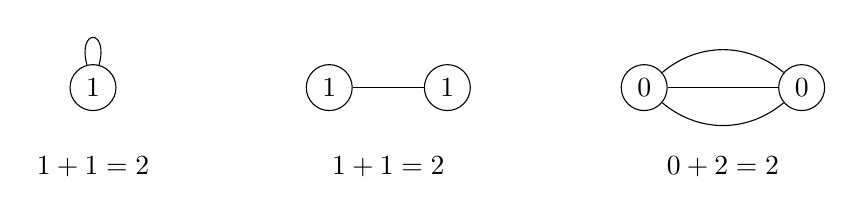
\begin{tikzpicture}[>=Stealth,v/.style={circle,draw,fill=white,inner sep=3pt}]
\node[v] (a) at (0,0) {$1$};\path (a) edge[loop above,looseness=8] (a);
\node[v] (b) at (3,0) {$1$};\node[v] (c) at (4.5,0) {$1$};\draw (b)--(c);
\node[v] (d) at (7,0) {$0$};\node[v] (e) at (9,0) {$0$};
\draw (d)--(e);\draw (d) to[bend left=40] (e);\draw (d) to[bend right=40] (e);
\node at (0,-1) {$1+1=2$};\node at (3.75,-1) {$1+1=2$};\node at (8,-1) {$0+2=2$};
\end{tikzpicture}
\end{center}
数字は正規化成分の種数であり、辺は節点である。これらの曲線はいずれも、次の安定性条件を満たす。
\end{minipage}\par\medskip

\subsection{安定性を正規化上で定義する}
\begin{dfn}[安定点付き曲線]\label{def:stable}
$2g-2+n>0$ とする。$n$ 点付き安定曲線は、算術種数 $g$ の節点曲線 $C$ と、滑らかな部分にある相異なる順序付き標点 $p_i$ で、各正規化成分について
\[
2g(C_v)-2+n_v>0
\]
を満たすものである。ここで $n_v$ は $C_v$ 上にある節点の\emph{逆像}と標点の総数である。
自己節点は同じ成分に二点を与える。
\end{dfn}
\begin{dfn}[安定曲線の族]
局所 Noether 的な $\C$-スキーム $S$ 上の $n$ 点付き安定曲線族は、proper flat な有限表示射 $\pi:C\to S$ と、滑らかな部分に値をもつ互いに交わらない切断 $s_i$ で、各幾何学的ファイバーが算術種数 $g$ の安定点付き曲線となるものである。
族の同型は $S$ 上で切断を保つ同型、基底を変える射は Cartesian な正方形とする。
全空間 $C$ の滑らかさは要求しない。
\end{dfn}
従って有理成分には三つ以上、種数 $1$ の成分には一つ以上の特別な点が必要である。
「他の成分との交点の数」だけを数えると、自己交点のある既約曲線で誤る。

\begin{prop}\label{prop:stablefinite}
節点付き曲線の安定性は、その標点を固定する自己同型群が有限であることと同値である。
\end{prop}
\begin{proof}
自己同型は正規化に持ち上がり、有限個の成分と特別な点を置換する。
この置換を自明にする部分群は、各 $(C_v;\text{特別な点})$ の自己同型群の積の部分群である。
安定なら命題\ref{prop:finiteaut}によって各因子が有限なので全体も有限である。

安定でない成分があれば、その正規化は特別な点を二つ以下しかもたない $\PP^1$、または特別な点のない種数 $1$ の曲線である。
命題\ref{prop:finiteaut}の無限自己同型群から各特別な点を固定する群を選び、他の成分上は恒等写像とする。
節点の二枝の貼り合わせを保つので $C$ の自己同型に降下し、無限群を得る。
\end{proof}

\subsection{双対化層とその次数}
\begin{dfn}[節点曲線の双対化層]\label{def:dualizing}
$\omega_C$ は、正規化上の有理型微分で、節点の逆像に高々単純極をもち、各節点で
\[
\operatorname{Res}_{q_e^+}\eta+\operatorname{Res}_{q_e^-}\eta=0
\]
を満たすものからなる層である。
節点では $dx/x=-dy/y$ によって生成される可逆層で、滑らかな部分では $\Omega_C^1$ に一致する。
\end{dfn}
この局所記述は節点が Gorenstein 特異点であることを具体的に表す。
$D=\sum p_i$ とし、成分 $C_v$ 上の節点の逆像の和を $N_v$、標点の和を $D_v$ とすると
\[
\nu^*\omega_C(D)|_{C_v}\simeq K_{C_v}(N_v+D_v).
\]
従ってその次数は $2g(C_v)-2+n_v$ である。

\begin{external}{曲線上の豊富性と双対性}\label{input:nodalduality}
被約射影曲線上の線束は、各既約成分上の次数が正であることと ample であることが同値である。
節点曲線では、上の $\omega_C$ は双対化層であり、任意の線束 $L$ に対して
$H^1(C,L)^\vee\simeq H^0(C,\omega_C\otimes L^{-1})$ が成り立つ。
出典：\cite{DM}, \S1、\cite{Hartshorne}, Chapter III の曲線の双対性。
\end{external}
\begin{cor}\label{cor:stableample}
点付き節点曲線は安定であることと $\omega_C(D)$ が ample であることが同値である。
\end{cor}
\begin{proof}
各成分の次数の式を豊富性判定に代入すれば、定義\ref{def:stable}の不等式そのものである。
\end{proof}

\begin{prop}[節点曲線の Riemann--Roch]
線束 $L$ に対して $\chi(C,L)=\deg L+1-g$ である。ここで $\deg L=\sum_v\deg(\nu^*L|_{C_v})$、$g=p_a(C)$ とする。
\end{prop}
\begin{proof}
正規化完全系列に線束 $L$ をテンソルする。
$L$ は局所自由なので完全性は保たれ、射影公式により中央項は $\nu_*\nu^*L$ となる。
右端は各節点での一次元のファイバー $L|_{q_e}$ をもつ点層である。
従って $L_v=\nu^*L|_{C_v}$ と書くと
\[
\chi(C,L)=\sum_v\chi(C_v,L_v)-|E|.
\]
各 $C_v$ は滑らかなので、既習の Riemann--Roch により $\chi(C_v,L_v)=\deg L_v+1-g_v$ である。
よって
\begin{align*}
\chi(C,L)
&=\sum_v\deg L_v+|V|-\sum_vg_v-|E|\\
&=\deg L+1-\bigl(\sum_vg_v+|E|-|V|+1\bigr)
=\deg L+1-g.
\end{align*}
最後の等号で正規化の種数公式を用いた。
\end{proof}

\begin{prop}\label{prop:plurih0}
標点のない安定曲線 $C$、$g\ge2$ と整数 $m\ge2$ に対して
\[
H^1(C,\omega_C^m)=0,\qquad h^0(C,\omega_C^m)=(2m-1)(g-1).
\]
\end{prop}
\begin{proof}
\textbf{1. 高次コホモロジーを負次数の切断に置き換える。}
節点曲線の双対性から
$H^1(\omega_C^m)^\vee\simeq H^0(\omega_C^{1-m})$ である。
安定性により各正規化成分上で $\deg\omega_C|_{C_v}=2g_v-2+n_v>0$ である。
$m\ge2$ なら $(1-m)(2g_v-2+n_v)<0$ なので、$\omega_C^{1-m}$ の切断は各成分で零となる。
正規化への引き戻しで切断は検出されるため、大域切断も零である。よって $H^1(\omega_C^m)=0$ となる。

\textbf{2. 双対化層の全次数を求める。}
各節点は正規化上に二つの点を与えるので $\sum_v n_v=2|E|$ である。
従って
\[
\deg\omega_C=\sum_v(2g_v-2+n_v)
=2\sum_vg_v-2|V|+2|E|=2g-2,
\]
最後の等号には命題\ref{prop:genusgraph}を使った。

\textbf{3. Riemann--Roch を適用する。}
消滅を用いると $h^0=\chi$ であり、節点曲線の Riemann--Roch から
\[
h^0(\omega_C^m)=m(2g-2)+1-g=(2m-1)(g-1)
\]
を得る。成分ごとの種数や節点の数に依存せず、算術種数だけで決まる点が、族の埋め込みに適している。
\end{proof}

\begin{external}{多重標準埋め込み}\label{input:pluricanonical}
$\pi:C\to S$ を標点のない安定曲線族、$g\ge2$ とする。
相対双対化層 $\omega_{C/S}$ は可逆で、任意の基底変換と可換である。
$m\ge3$ なら $\omega_{C/S}^m$ は relatively very ample である。
出典：Edidin \cite{Edidin}, Theorem 3.1、Deligne--Mumford \cite{DM}, \S1。
\end{external}
\begin{cor}\label{cor:relativecanonical}
$m\ge3$ に対し、$V=\pi_*\omega_{C/S}^m$ は階数 $r=(2m-1)(g-1)$ の局所自由層で基底変換と可換であり、評価は閉埋め込み
$C\hookrightarrow\PP_S(V^\vee)$ を与える。
\end{cor}
\begin{proof}
$L=\omega_{C/S}^m$ と置く。
相対双対化層の基底変換により、幾何学的ファイバーへの制限は $L_{\bar s}=\omega_{C_{\bar s}}^m$ である。
前の命題を各ファイバーに適用すると $H^1(L_{\bar s})=0$、$h^0(L_{\bar s})=r$ が得られる。
ここで種数は族で一定なので $r$ も一定である。
従って引用定理\ref{input:basechange}の前半から $V=\pi_*L$ は階数 $r$ の局所自由層となり、任意の基底変換と可換である。
引用定理\ref{input:pluricanonical}により $m\ge3$ では各 $L_{\bar s}$ は very ample である。
そこで基底変換定理の後半を適用すれば、評価 $\pi^*V\to L$ による閉埋め込みを得る。
$V$ の局所基底を選べば、その基底の切断の値を射影座標として書いたものがこの埋め込みである。
\end{proof}
ここでは「各成分で正次数だから very ample」とは推論していない。正次数は ample 性であり、$m\ge3$ の very ample 性は別の定理である。

\subsection{節点の変形と境界の局所方程式}
$\mathcal T_C=\mathcal Hom(\Omega_C^1,\OO_C)$、
$\mathcal T_C^1=\mathcal Ext^1(\Omega_C^1,\OO_C)$ と書く。
$\Ext^i$ は $\Hom$ の右導来関手、$\mathcal Ext^i$ はその層版である。
\begin{external}{節点曲線の変形理論}\label{input:nodaldef}
節点曲線 $C$ の一次変形は $\Ext^1(\Omega_C^1,\OO_C)$、障害は $\Ext^2(\Omega_C^1,\OO_C)$ で記述される。
局所大域スペクトル系列から
\[
0\to H^1(C,\mathcal T_C)\to\Ext^1(\Omega_C^1,\OO_C)
\to H^0(C,\mathcal T_C^1)\to0
\]
が完全であり、$\Ext^2=0$ である。
さらにこの変形は有効で、安定曲線には滑らかな解析的普遍変形の芽がある。
出典：\cite{DM}, \S1 の変形理論、\cite{Sernesi}, Chapter 3 の局所大域変形。
\end{external}
\begin{prop}\label{prop:nodaldim}
節点が $\delta$ 個ある種数 $g\ge2$ の安定曲線は、$3g-3$ 次元の局所変形空間をもつ。
そのうち $\delta$ 個の独立なパラメータが各節点を平滑化し、局所的に境界は $t_1\cdots t_\delta=0$ である。
\end{prop}
\begin{proof}
\textbf{1. 一つの節点を平滑化する方向は一次元である。}
$R=\C[[x,y]]/(xy)$ では、以下の微分と導分を完備局所環に適合する連続な意味で取る。完備化された微分加群は $dx,dy$ で生成され、関係は $y\,dx+x\,dy=0$ である。
従って
\[
0\longrightarrow R\xrightarrow{a\mapsto(ay,ax)}R^2
\longrightarrow\Omega_R^1\longrightarrow0
\]
を得る。左の単射性を確認しよう。$ax=ay=0$ なら、$a$ を正規化環の組 $(f(x),g(y))$ で表すと、
$xf(x)=0$、$yg(y)=0$ なので $f=g=0$、従って $a=0$ である。
この自由分解に $\Hom_R(-,R)$ を適用すると
\[
\Ext_R^1(\Omega_R^1,R)
=\coker\{R^2\xrightarrow{(b,c)\mapsto by+cx}R\}
=R/(x,y)=\C.
\]
局所方程式 $xy-a\eps=0$ の係数 $a$ がこの方向を与え、その実際の平滑化は $xy=t$ である。
従って $\mathcal T_C^1$ は各節点に一次元ずつ載る点層で、$h^0(\mathcal T_C^1)=\delta$ である。

\textbf{2. 節点を保ったまま変形する方向を求める。}
節点の導分 $D$ には $yD(x)+xD(y)=0$ が必要である。
$x$ の枝へ制限すると $D(y)|_{y=0}=0$、$y$ の枝では $D(x)|_{x=0}=0$ となる。
従って正規化上のベクトル場は二つの節点逆像で消える。
逆にそのようなベクトル場は、定数項が等しい関数の組を保つので導分に降りる。
よって
\[
\mathcal T_C\simeq\nu_*\Bigl(\bigoplus_vT_{C_v}(-N_v)\Bigr).
\]
各成分は安定範囲にあり、第\ref{sec:def}節の標点付き計算から
$h^1(T_{C_v}(-N_v))=3g_v-3+n_v$ である。
$v=|V|$ と略記すると
\begin{align*}
h^1(\mathcal T_C)
&=3\sum_vg_v-3|V|+2\delta\\
&=3(g-\delta+|V|-1)-3|V|+2\delta
=3g-3-\delta.
\end{align*}

\textbf{3. 二種類の方向を合わせる。}
引用定理\ref{input:nodaldef}の完全系列で右端は $\C^\delta$ なので
\[
\dim\Ext^1(\Omega_C^1,\OO_C)
=(3g-3-\delta)+\delta=3g-3.
\]
右への全射性は、各節点の平滑化方向を独立に指定できることを意味する。
障害の消滅と変形の存在定理により、変形空間の芽はこの次元で滑らかである。
局所方程式 $xy=t_e$ のパラメータをすべて集めた写像は微分が全射なので、解析的な陰関数定理により $t_1,\ldots,t_\delta$ を座標の一部に選べる。
十分小さい近傍では元の節点の外は滑らかなままであり、曲線が滑らかである条件はすべての $t_e$ が非零となることに等しい。
従って境界は $\{t_1\cdots t_\delta=0\}$ である。
\end{proof}
これはスタックの滑らかな局所 atlas 上の正規交叉の記述である。自己同型群で割った粗空間で、同じ座標がそのまま座標になるとは限らない。

\begin{exa}[二つの節点がある場合]
節点のない部分を変形する座標を $s_1,\ldots,s_{3g-5}$ とすると、局所変形空間には
$(s_1,\ldots,s_{3g-5},t_1,t_2)$ という座標を取れる。
$t_1=0,t_2\neq0$ では第一の節点だけが残り、$t_1\neq0,t_2=0$ では第二だけが残る。
$t_1=t_2=0$ は二節点を保つ部分で、余次元二である。
\end{exa}
\par\medskip
\noindent\begin{minipage}{\linewidth}
\begin{center}
\begin{tikzpicture}[>=Stealth]
\fill[green!4] (-2,-1.5) rectangle (2,1.5);
\draw[->] (-2.3,0)--(2.5,0) node[right] {$t_1$};
\draw[->] (0,-1.7)--(0,1.9) node[above] {$t_2$};
\draw[very thick,blue!55!black] (-2,0)--(2,0);
\draw[very thick,green!45!black] (0,-1.5)--(0,1.5);
\fill (0,0) circle(2pt);
\node[align=left] at (5,.8) {軸の外：両方を平滑化\\横軸：第二節点が残る\\縦軸：第一節点が残る};
\node[align=left] at (5,-.9) {原点：二節点が残る\\他の $s$ 座標は固定};
\end{tikzpicture}
\end{center}
\end{minipage}\par\medskip
図は複素二次元の $(t_1,t_2)$ 空間の実断面である。境界の二成分を表す図であり、曲線自体を描いたものではない。

\par\bigskip\Needspace{.70\textheight}
\section{Hilbert スキームと曲線スタックの表示}\label{sec:hilbert}
\begin{aim}
曲線の埋め込みを選ぶ空間を作り、座標の選択を忘れる操作を商スタックで表す。対象の対応だけでなく、同型射の対応まで確認する。
\end{aim}
\subsection{Hilbert 関手}
\begin{dfn}
閉部分スキーム $Z\subset\PP^N$ の Hilbert 多項式は
$P_Z(t)=\chi(Z,\OO_Z(t))$ によって定まる多項式である。
固定した $P$ に対し、Hilbert 関手は基底 $S$ を
\[
\Hilb_P(\PP^N)(S)=\{Z\hookrightarrow\PP^N_S\mid Z\to S\text{ は flat、各幾何学的ファイバーの Hilbert 多項式は }P\}
\]
に送る。ここでは埋め込みを含めて記録し、同じ閉部分スキームを同一視する。
\end{dfn}
\begin{external}{Hilbert スキームの存在}\label{input:hilbert}
この関手は射影スキーム $\Hilb_P(\PP^N)$ で表現され、普遍閉部分スキーム
$\mathscr Z\subset\PP^N\times\Hilb_P(\PP^N)$ をもつ。
十分大きい整数 $k$ について、$H^0(\PP^N,\OO(k))$ の階数 $P(k)$ の商を取る写像により、Hilbert スキームは Grassmann 多様体に閉埋め込みされる。
出典：\cite{FGA} の Hilbert scheme、Edidin \cite{Edidin}, \S\S3.2, 4.4。
\end{external}
曲線の同型類ではなく、\emph{射影空間内の位置}を分類するため、ここでは普遍族が存在する。
自己同型の問題は、射影座標の変更を忘れる次の段階で現れる。

\subsection{多重標準曲線の部分空間}
$g\ge2$、$m\ge3$ を固定し、
\[
d=m(2g-2),\quad r=(2m-1)(g-1),\quad N=r-1=d-g,\quad P(t)=dt+1-g
\]
とする。命題\ref{prop:plurih0}と Riemann--Roch がこれらの数を与える。
\begin{external}{多重標準 Hilbert 部分スキーム}\label{input:canonicalhilbert}
$\Hilb_P(\PP^N)$ には、完全 $m$ 重標準系によって埋め込まれた安定曲線を分類する有限型局所閉部分スキーム $\overline H_{g,m}$ が存在する。
その開部分 $H_{g,m}$ は滑らかな曲線を分類する。
この主張は族についてのものであり、$S\to\overline H_{g,m}$ は、相対的に完全な埋め込み $C\hookrightarrow\PP^N_S$ が局所的に $\omega_{C/S}^m$ によって与えられることを意味する。
より正確には $\OO_C(1)\otimes\omega_{C/S}^{-m}$ の相対 Picard 類が零であることを要求する。
出典：Edidin \cite{Edidin}, \S3.2 と Theorem 3.2 の直前の構成、\cite{DM}, \S5。
\end{external}
相対 Picard 類が零とは、局所的に基底からの線束の引き戻しになるという意味である。
従って $\OO_C(1)$ と $\omega_{C/S}^m$ の同型を一つ選ぶことは、$\overline H_{g,m}$ のデータには含めない。
その同型を選ぶと、不要なスカラーの自由度を追加してしまう。
また幾何学的ファイバーごとの線束の同型だけを要求すると、非被約基底上の相対 Picard 方向を排除できない。
ここでは上の関手的・スキーム的な条件を用いる。

$G=\PGL_r$ は射影座標の変更で $\overline H_{g,m}$ に作用する。
\begin{lem}[固定点群]\label{lem:hilbstab}
$h\in\overline H_{g,m}(\C)$ に対応する曲線を $C$ とすると、$G_h\simeq\Aut(C)$ である。
\end{lem}
\begin{proof}
\textbf{1. 制限によって準同型を作る。}
射影変換 $A\in G_h$ は埋め込み像 $C\subset\PP^{r-1}$ を保つので、制限 $A|_C$ は $C$ の自己同型である。
従って $G_h\to\Aut(C)$ という群準同型がある。

\textbf{2. 自己同型を射影空間全体へ延長する。}
$f\in\Aut(C)$ は双対化層の関手性により $f^*\omega_C\simeq\omega_C$ を与え、
$V=H^0(C,\omega_C^m)$ に可逆線形写像 $f^*:V\to V$ を誘導する。
その双対の射影化によって、完全線形系の射影空間上に $f$ を延長する射影変換を得る。
評価写像による埋め込みの関手性から、曲線上の制限はもとの $f$ である。
ここでは完全線形系を使っていることが必要である。

\textbf{3. 延長が一意であることを確認する。}
曲線上恒等な射影変換 $A$ を考える。
$A$ が $\OO_C(1)$ に誘導する同型は、恒等写像の上の線束自己同型なので、
$H^0(C,\OO_C^*)=\C^*$ に属する一つの定数倍である。
座標の制限 $H^0(\PP^{r-1},\OO(1))\to H^0(C,\OO_C(1))$ は完全系による埋め込みだから同型である。
従って $A$ を表す線形写像もスカラーであり、射影変換として $A=1$ となる。
これで二つの構成が互いに逆であることがわかった。

同じ構成は任意の基底変換と可換である。
族では $\pi_*\OO_C=\OO_S$（幾何学的に連結な被約 proper 曲線の基底変換定理）を用い、上のスカラーを基底上の可逆関数と読み替える。
従って対象の自己同型関手まで同一視でき、群スキームとしても同型となる。
\end{proof}

\begin{exa}[種数二、三重標準系で数値を確認する]
$g=2,m=3$ なら $d=6$、$r=5$、$N=4$、$P(t)=6t-1$ である。
従って $\overline H_{2,3}$ は $\PP^4$ 内の次数六の曲線を分類する Hilbert スキームの部分である。
同じ抽象曲線でも、$H^0(\omega_C^3)$ の基底を替えると $\PP^4$ 内の位置が変わる。
この変更の群は $\PGL_5$ で次元は $25-1=24$ である。
曲線そのものの変形は $3g-3=3$ 次元なので、後の滑らかさの定理を使えば $\overline H_{2,3}$ の次元は $3+24=27$ となる。
Hilbert スキームで分類するデータが、曲線の同型類より多いことをこの数字からも確認できる。
\end{exa}

\subsection{族から主束を作る}
\begin{dfn}
$\overline{\mathcal F}_g(S)$ を $S$ 上の安定曲線族と $S$ 上の同型からなる亜群とする。
$\mathcal F_g$ はその滑らかな族からなる部分亜群とする。
\end{dfn}
\begin{thm}[商表示]\label{thm:hilbertquotient}
自然な同値
\[
\overline{\mathcal F}_g\simeq[\overline H_{g,m}/\PGL_r],\qquad
\mathcal F_g\simeq[H_{g,m}/\PGL_r]
\]
がある。出典となる構成は Edidin, Theorem 3.2 である。
\end{thm}
\begin{proof}
$H=\overline H_{g,m}$、$G=\PGL_r$ と略記する。
\textbf{方針。} 任意の基底 $S$ について二つの亜群の間に関手を作り、対象を復元できることと、同型射も一対一に対応することを示す。

\textbf{1. 曲線の族を、射影座標を選べる主束へ引き戻す。}
安定曲線族 $\pi:C\to S$ に対して $V=\pi_*\omega_{C/S}^m$ と置く。
系\ref{cor:relativecanonical}により $V$ は階数 $r$ であり、評価による標準的な閉埋め込み
$j:C\hookrightarrow\PP_S(V^\vee)$ がある。
$T\to S$ 上の射影枠を、同型
\[
p:\PP_T(V_T^\vee)\xrightarrow{\sim}\PP^{r-1}_T
\]
とする。これらを表すスキームを $P$ と書く。
$V$ が自明な開集合では $P\simeq S\times\PGL_r$ であるから、$P\to S$ は主束である。
右作用を $p\cdot g=g^{-1}\circ p$ と定める。

$P$ 上にはその点自身が指定する射影枠がある。
従って $C_P$ は $\PP^{r-1}_P$ に埋め込まれ、Hilbert 関手の普遍性により一意な射 $u:P\to H$ を定める。
枠 $p$ を $p\cdot g$ に替えると埋め込み像は $g^{-1}$ 倍されるので、
$u(pg)=g^{-1}u(p)$ である。
よって $(P,u)$ は $[H/G](S)$ の対象である。

\textbf{2. 主束と同変写像から局所曲線を作る。}
逆に $(P\to S,u:P\to H)$ を与える。
$P$ を自明化する étale 被覆 $\{S_i\to S\}$ と切断 $p_i:S_i\to P$ を選び、$u_i=u\circ p_i$ と置く。
$u_i$ に沿って $H$ 上の普遍埋め込み曲線を引き戻し、
$C_i\subset\PP^{r-1}_{S_i}$ を得る。
重なりで $p_j=p_i g_{ij}$ と書くと $u_j=g_{ij}^{-1}u_i$ なので、射影変換 $g_{ij}$ は
\[
\phi_{ij}:C_j|_{S_{ij}}\xrightarrow{\sim}C_i|_{S_{ij}}
\]
を与える。
$g_{ij}g_{jk}=g_{ik}$ より $\phi_{ij}\phi_{jk}=\phi_{ik}$ であり、曲線の降下データを得た。

\textbf{3. 降下がスキームとして有効である理由を確認する。}
対象を貼り合わせるには、単に cocycle 条件を書くだけでなく有効降下の定理が必要である。
各 $C_i$ は相対 ample 線束 $\omega_{C_i/S_i}^m$ をもち、$\phi_{ij}$ は双対化層の関手性によって、この線束の適合する同型も与える。
従って引用定理\ref{input:descent}の「ample 線束を備えた射影的スキーム」の場合を適用でき、$S$ 上の射影的スキーム $C$ が得られる。
flat 性、節点ファイバー、安定性は étale 局所的に検査できるので $C\to S$ は安定曲線族である。
ここでは射影空間の $\OO(1)$ に $\PGL_r$ の線型化を選んだのではなく、曲線の標準的な線束 $\omega^m$ を用いた。

\textbf{4. 対象について二つの構成が逆であることを示す。}
曲線族 $C$ から始めた場合、第2段階の $C_i$ は元の曲線に局所的な射影座標を付けたものにすぎない。
降下同型も元の曲線の同一視なので、有効降下の一意性から元の $C$ に戻る。

$(P,u)$ から始めた場合には、降下した $C$ の完全多重標準射影枠を $P'$ とする。
$P$ 上にあった埋め込みは、その完全性と $\OO(1)\otimes\omega^{-m}$ の相対 Picard 類が零であることにより、$P$ 上の射影枠を定める。
基底からの線束のテンソルは射影束を変えないため、線束の同型を別途選ぶ必要はない。
こうして同変射 $P\to P'$ が得られる。
主束間の同変射は、局所自明化すると $G$ の平行移動となり同型である。
この同型は Hilbert 写像とも可換なので、元の $(P,u)$ が復元される。

\textbf{5. 同型射についても一対一であることを示す。}
族の同型 $f:C\to C'$ は双対化層の引き戻し、切断空間、そして射影束の同型を誘導する。
従って射影枠を運ぶ主束同型 $P\to P'$ を与え、埋め込み像の対応により $u$ と $u'$ に適合する。
逆にそのような主束同型があれば、共通の被覆上で二つの埋め込み曲線の同型が得られる。
これらは降下データと可換なので、一意な $S$ 上の曲線同型に降下する。
局所的には完全線形系からの構成が互いに逆だから、これらはすべての同型射を一対一に対応させる。

従って得られた関手は fully faithful（各同型集合上で全単射）かつ essentially surjective（各対象が像の対象と同型）であり、亜群の同値である。
双対化層と直像は基底変換と可換なので、同値は $S$ について自然である。
滑らかな曲線に制限してもすべての構成が保たれ、第二の同値を得る。
\end{proof}
\par\medskip
\noindent\begin{minipage}{\linewidth}
\begin{center}
\begin{tikzcd}[column sep=large,row sep=large]
C_P\ar[r]\ar[d]&\mathscr Z_H\ar[d]\\
P\ar[r,"u"]\ar[d,swap,"\text{射影枠の主束}"]&H\ar[d]\\
S\ar[r]&{[H/G]}
\end{tikzcd}
\end{center}
上段で埋め込みを含む族を分類し、下段で射影座標の選択を忘れる。
$C_P$ の降下データを保って忘れるため、曲線の自己同型は商スタックに残る。
\end{minipage}\par\medskip

この証明で $\GL_r$ ではなく $\PGL_r$ を用いたのは、共通スカラー倍が射影座標を変えないためである。

\subsection{DM 性と滑らかさ}
\begin{external}{安定曲線の同型関手}\label{input:isomfinite}
二つの安定曲線族 $C,C'\to S$ に対し、$\Isom_S(C,C')$ は有限かつ unramified な $S$-スキームで表現される。
出典：\cite{DM}, Theorem 1.11、および Edidin \cite{Edidin}, \S2.2。
特に幾何学的ファイバーの自己同型群スキームは有限被約である。
\end{external}
\begin{thm}\label{thm:dmcurves}
$\overline{\mathcal F}_g$ は有限型の分離的な DM スタックであり、これを $\cM_g$ と書く。
滑らかな曲線の部分 $\MM_g$ は開部分スタックである。
両者は $\C$ 上滑らかで次元 $3g-3$ である。
\end{thm}
\begin{proof}
\textbf{1. スタックの存在と有限型性。}
前の定理は曲線族の亜群を $[\overline H_{g,m}/\PGL_r]$ と同一視する。
商は命題\ref{prop:quotstack}によりスタックであり、有限型スキーム $\overline H_{g,m}$ から smooth surjective atlas をもつ。
従って有限型の algebraic stack である。

\textbf{2. DM 性と分離性。}
対角の任意の基底変換は補題\ref{lem:diagonal}により二つの族の $\Isom$ 関手である。
引用定理\ref{input:isomfinite}によればこれは有限 unramified である。
unramified な対角と smooth atlas に DM 判定定理を適用して DM 性を得る。
また有限射は proper なので対角は proper、従ってスタックは separated である。
DM 性に用いる unramified と、分離性に用いる proper をここで区別している。

\textbf{3. 滑らかな曲線の部分が開であること。}
有限表示射の smooth locus は全空間の開集合である。
proper な族ではその補集合の像は閉なので、その像の補集合が「ファイバー全体が滑らか」という条件を表す開集合となる。
この条件を Hilbert atlas で調べれば $H_{g,m}$ は開であり、対応する部分スタック $\MM_g$ も開である。

\textbf{4. スタック自体の滑らかさと次元。}
節点曲線の変形定理により、任意の点で small extension に対する持ち上げ障害が消滅する。
有限型のスタックの smoothness の無限小判定を使うと、$\cM_g\to\Spec\C$ は smooth である。
より具体的には étale atlas の点の局所変形は、もとの曲線の変形と一致する。
étale 射には無限小持ち上げの一意性があるため、atlas の接空間は曲線の変形接空間に等しい。
命題\ref{prop:nodaldim}よりこの次元は $3g-3$ である。
従って atlas は滑らかで次元 $3g-3$、そしてスタックもその次元となる。
開部分 $\MM_g$ にも同じ結論が成り立つ。
\end{proof}
ここでは無限小の変形が実際の有限型スタックの滑らかさを検査できるという、smoothness の無限小判定も用いた。
解析的な有限商模型だけから、代数的なスタックの存在を逆算しているわけではない。

\begin{rem}[atlas の次元]
$\overline H_{g,m}\to\cM_g$ は相対次元 $\dim\PGL_r=r^2-1$ の smooth atlas である。
従って $\dim\overline H_{g,m}=(3g-3)+(r^2-1)$ となる。
座標を選ぶための自由度と、曲線自体を動かす自由度がここで分離される。
\end{rem}

\par\bigskip\Needspace{.70\textheight}
\section{GIT と粗モジュライ空間の構成}\label{sec:git}
\begin{aim}
群の軌道集合に代数空間の構造を入れるための条件を整理する。Hilbert 点の安定性定理を、曲線の安定性と区別して適用する。
\end{aim}
\subsection{よい商と幾何学的商}
\begin{dfn}
代数群 $G$ が $X$ に作用するとき、不変射 $q:X\to Y$ が good quotient であるとは、次を満たすことをいう。
\begin{enumerate}
\item $q$ は affine かつ全射で、$\OO_Y\xrightarrow{\sim}(q_*\OO_X)^G$ である。
\item $G$-不変閉集合の像は閉である。
\item 互いに交わらない二つの $G$-不変閉集合の像は交わらない。
\end{enumerate}
さらに幾何学的ファイバーが一つの軌道であるとき geometric quotient と呼ぶ。
\end{dfn}
不変式の環を取る操作は軌道の閉包の情報を記録する。
\begin{exa}[不変式が二つの軌道を区別できない場合]
$\C^*$ が $\A^2$ に $t\cdot(x,y)=(tx,t^{-1}y)$ で作用すると、不変式環は $\C[xy]$ であり、商は $(x,y)\mapsto xy$ で与えられる。
非零ファイバーは一軌道だが、零ファイバーには原点と二つの非閉軌道がある。
従ってこの good quotient は全体では geometric quotient ではない。
これを計算で確認すると、単項式 $x^ay^b$ の重みは $a-b$ だから、不変な単項式は $(xy)^a$ に限られる。
異なる重みの項は打ち消し合わないので、不変式環はちょうど $\C[xy]$ となる。
$c\neq0$ に対して $xy=c$ の二点 $(x,y),(x',y')$ を取ると、$t=x'/x$ によって一方から他方へ移れる。
一方、$xy=0$ の三つの軌道は
\[
O_x=\{(x,0):x\neq0\},\quad
O_y=\{(0,y):y\neq0\},\quad O_0=\{(0,0)\}
\]
である。$\overline O_x$ と $\overline O_y$ はともに $O_0$ を含む。
多項式不変量は連続で軌道上一定なので、これら三つに別々の値を与えることはできない。
\end{exa}

\par\medskip
\noindent\begin{minipage}{\linewidth}
\begin{center}
\begin{tikzpicture}[>=Stealth,scale=.85]
\draw[->] (-2.3,0)--(2.4,0) node[right] {$x$};
\draw[->] (0,-1.9)--(0,2) node[above] {$y$};
\draw[very thick,blue!60!black] (-2,0)--(-.08,0) (.08,0)--(2,0);
\draw[very thick,green!50!black] (0,-1.7)--(0,-.08) (0,.08)--(0,1.7);
\fill (0,0) circle(2.5pt);
\draw[orange!75!black,thick,domain=.65:2,samples=40] plot (\x,{1/\x});
\draw[orange!75!black,thick,domain=-2:-.65,samples=40] plot (\x,{1/\x});
\draw[->] (3,0)--(5,0) node[midway,above] {$q(x,y)=xy$};
\draw[->] (5.7,0)--(9,0) node[right] {$c$};
\fill (6.3,0) circle(2pt) node[below] {$0$};
\fill[orange!75!black] (7.7,0) circle(2pt) node[below] {$1$};
\node[align=center] at (6.4,1.2) {零ファイバーの\\三軌道を一つに};
\end{tikzpicture}
\end{center}
図は実断面である。複素数体上では $xy=1$ 全体が一つの $\C^*$ 軌道となる。
\end{minipage}\par\medskip

\begin{external}{good quotient の普遍性と固定点群}
good quotient は不変射に関して categorical である。すなわち不変射 $X\to Z$ は一意に $X\to Y\to Z$ と因子化する。
また、有限被約固定点群をもつ局所 proper な作用の geometric quotient $q:X\to Y$ が universally submersive なら、$[X/G]\to Y$ は粗モジュライ空間である。
ここで局所 proper とは、不変開集合で覆って各作用射 $G\times U\to U\times U$ が proper となることであり、universally submersive とは任意の基底変換後にも商位相を与えることである。
出典：Edidin \cite{Edidin}, Propositions 4.1, 4.2 とその直前の仮定、\cite{Vistoli}, Proposition 2.11。
代数空間を標的とする普遍性もこの商定理に含めて用いる。
\end{external}
射 $[X/G]\to Y$ の構成自体は具体的である。
対象 $(P\to S,u:P\to X)$ に対し $q\circ u$ は $G$-不変なので、$P\to S$ の降下によって一意な $S\to Y$ を与える。
幾何学的点上では、代数閉体上の主束は自明化でき、geometric quotient の軌道と対象の同型類が一致する。
最後の普遍性と proper 性のために上の商定理の仮定が必要である。

\subsection{線型化と安定点}
\begin{dfn}
線束 $L$ の $G$-linearization は、$G$ の作用を $L$ の全空間にファイバー上線形に持ち上げ、群の合成則を満たす作用である。
射影スキーム $X$ と ample な linearized 線束 $L$ に対して、$x\in X$ が semistable であるとは、ある $n>0$ と $s\in H^0(X,L^n)^G$ があり $s(x)\neq0$ となることをいう。
semistable locus を $X^{ss}(L)$ とする。
$Gx$ が $X^{ss}(L)$ の中で閉じ、固定点群が有限となる $x$ を stable と呼び、$X^s(L)$ と書く。
\end{dfn}
以下の $G$ は $\SL_r$ または $\PGL_r$ であり、これらは reductive 群である。
一般に reductive とは連結 unipotent 正規部分群をもたない線型代数群をいう。
標数 $0$ では reductive 群の不変式に有限生成定理を適用できる。

\begin{external}{GIT の商定理}\label{input:git}
$G$ を reductive、$X$ を射影スキーム、$L$ を ample な linearized 線束とする。
不変切断環 $R=\bigoplus_{n\ge0}H^0(X,L^n)^G$ は有限生成で、
\[
q:X^{ss}(L)\longrightarrow X/\!/_{L}G:=\Proj R
\]
は good quotient である。右辺は射影スキームである。
$X^s(L)$ は商のある開部分の逆像であり、その制限は universally submersive な geometric quotient となる。
stable locus 上の作用は proper であり、固定点群は有限である。
出典：\cite{GIT}, Chapter 1、Edidin \cite{Edidin}, Theorem 4.1 と \S4.1 の末尾。
\end{external}
安定点の商だけでは、一般には射影性は得られない。
商の射影性を得るには、対象とする部分が\emph{半安定部分の中で閉じている}ことも必要になる。

\subsection{Hilbert--Mumford 判定と符号の規約}
$X\subset\PP(V)$ を、点が $V$ の一次元部分空間を表す規約で埋め込む。
一点 $x=[v]$ と $1$-parameter subgroup $\rho:\C^*\to G$ をとり、
$\rho(t)e_i=t^{w_i}e_i$、$v=\sum v_ie_i$ と対角化する。
\begin{dfn}
本ノートでは $\mu(x,\rho)=-\min\{w_i\mid v_i\neq0\}$ とする。
\end{dfn}
\begin{external}{Hilbert--Mumford 判定}\label{input:hm}
$x$ は semistable であることと、すべての $1$-parameter subgroup に対して $\mu(x,\rho)\ge0$ であることが同値である。
$x$ は stable であることと、すべての非自明な $1$-parameter subgroup に対して $\mu(x,\rho)>0$ であることが同値である。
出典：\cite{GIT}, Chapter 2、Edidin \cite{Edidin}, Theorem 4.2。
\end{external}
例えばすべての非零座標の重みが正なら、$t\to0$ で $\rho(t)v\to0$ である。
不変同次多項式は軌道上一定なので、$v$ で非零となる正次数不変式は存在しない。従ってこの点は不安定である。
この必要条件から十分条件を導く部分が判定定理の深い内容である。

\begin{prop}[二変数四次形式]\label{prop:quarticgit}
$\SL_2$ の自然な作用に関し、二変数四次形式 $f$ の点が semistable であることは、$\PP^1$ 上の各根の重複度が $2$ 以下であることと同値である。
stable であることは四根がすべて異なることと同値である。
\end{prop}
\begin{proof}
\textbf{1. 一つの一径数部分群について重みを計算する。}
任意の非自明な一径数部分群は、適当な基底で
$X\mapsto t^rX$、$Y\mapsto t^{-r}Y$、$r>0$ と書ける。
$X^iY^{4-i}$ に掛かる係数は $t^{ri-r(4-i)}=t^{(2i-4)r}$ なので、重みは次の通りである。
\[
\begin{array}{c|ccccc}
\text{単項式}&Y^4&XY^3&X^2Y^2&X^3Y&X^4\\\hline
\text{重み}&-4r&-2r&0&2r&4r
\end{array}
\]
$f=\sum_{i=0}^4a_iX^iY^{4-i}$ と書く。
$[0:1]$ 付近の座標 $z=X/Y$ では $f/Y^4=\sum a_i z^i$ であるから、根の重複度 $m$ は最初の非零係数の添字である。
根でなければ $m=0$ とする。
従って最小の非零重みは $(2m-4)r$、本ノートの符号規約で
\[
\mu([f],\rho)=(4-2m)r
\]
となる。これは $m\le2$ のとき非負、$m<2$ のとき正である。

\textbf{2. すべての一径数部分群を調べる。}
一つの対角部分群だけを調べたのでは不十分である。
基底を替えることにより $\PP^1$ の任意の点を $[0:1]$ にでき、すべての一径数部分群はそのような基底で対角化される。
従ってすべての $\rho$ に対する条件は、すべての点で根の重複度が $2$ 以下、または $2$ 未満であることに等しい。
引用定理\ref{input:hm}を適用して、半安定条件と安定条件を得る。
四次形式で全根の重複度が $2$ 未満であるとは、四つの根がすべて相異なることである。
\end{proof}
曲線の「節点のみ、成分上の特別な点の数」という安定性と、ここでの GIT 安定性は定義が異なる。
両者を結び付けるには次の定理が必要である。

\subsection{Hilbert 点と Gieseker の定理}
$P(t)=dt+1-g$ とする。十分大きい $k$ では制限は階数 $P(k)$ の商
\[
W_k:=H^0(\PP^N,\OO(k))\twoheadrightarrow H^0(C,\OO_C(k))
\]
を与える。その最上外積は一次元商
$\bigwedge^{P(k)}W_k\twoheadrightarrow\det H^0(C,\OO_C(k))$ となり、対応する点を $k$ 次 Hilbert 点と呼ぶ。
従って埋め込み先は $\PP((\bigwedge^{P(k)}W_k)^\vee)$ である。
$m$ は多重標準埋め込みの冪、$k$ は Hilbert 点を作る次数であり、二つを区別する。

\begin{external}{Gieseker の構成で用いる入力}\label{input:gieseker}
$g\ge3$、$d\ge20(g-1)$、$N=d-g$ とする。
ある十分大きい整数 $k_0$ が存在し、次が成立する。
\begin{enumerate}
\item 完全線型系によって埋め込まれた滑らかな次数 $d$、種数 $g$ の曲線の $k_0$ 次 Hilbert 点は $\SL_{N+1}$-stable である。
\item 同じ $k_0$ による semistable Hilbert 点は、連結被約節点曲線で、各滑らかな有理成分が残りと少なくとも二点で交わる半安定曲線を与える。
\item $d=m(2g-2)$ として、semistable Hilbert locus $U$ 内で $\OO_C(1)$ の相対 Picard 類が $\omega_C^m$ と一致する部分 $U_c$ は閉部分スキームである。
それは $\overline H_{g,m}$ に一致し、すべての安定曲線の完全 $m$ 重標準埋め込みを含む。
\end{enumerate}
出典：Edidin \cite{Edidin}, Theorems 4.3, 4.4 と \S4.4 末尾、Gieseker \cite{Gieseker}, Theorems 1.0.0, 1.0.1, 2.0.1。
本ノートでは $m\ge10$ としてこの数値条件を満たす。
ここで存在する $k_0$ を固定して使い、原著より強い「任意の十分大きい $k$」への置き換えはしない。
\end{external}
この長い安定性証明は本ノートでは再現しない。
特に「安定曲線なら GIT 安定」という主張を定義として使っているわけではない。

\begin{lem}[有限固定点群から安定性へ進むための閉性]\label{lem:closedorbits}
上の $U_c$ のすべての点は GIT stable である。
\end{lem}
\begin{proof}
\textbf{方針。} 閉じていない軌道には、その閉包の境界に次元の小さい軌道が必要である。
しかし今回の部分では、固定点群がすべて有限なので軌道次元が下がれない。

$G=\PGL_{N+1}$ とし、$x\in U_c$ の軌道を $O=Gx$ とする。
$U_c$ は半安定部分 $U$ の中で不変かつ閉なので、$U$ 内の閉包 $\overline O$ も $U_c$ に含まれる。
$O$ が閉でないと仮定し、$y\in\overline O\setminus O$ を取る。
代数群の軌道は局所閉であり、$O$ は自分の閉包の開稠密部分だから
\[
\dim(Gy)\le\dim(\overline O\setminus O)<\dim O.
\]
一方、$x,y$ はいずれも安定曲線の多重標準点である。
固定点群の同定と安定曲線の自己同型の有限性により、$\dim G_x=\dim G_y=0$ である。
軌道の次元公式から
\[
\dim O=\dim G-\dim G_x=\dim G
=\dim G-\dim G_y=\dim(Gy),
\]
となり矛盾する。
従って軌道は半安定部分内で閉であり、固定点群も有限なので stable である。
$\SL_{N+1}$ で考えても有限中心を除けば同じ軌道・同じ次元なので結論は変わらない。
\end{proof}
有限固定点群だけから安定性を結論することはできない。上の証明では $U_c$ の閉性も使っている。

\begin{thm}[射影的な粗モジュライ空間]\label{thm:projectivecoarse}
$g\ge3$ に対し、安定曲線の粗モジュライ空間 $\overline M_g$ は射影スキームとして存在する。
滑らかな曲線の粗モジュライ空間 $M_g$ はその開部分であり、準射影的である。
\end{thm}
\begin{proof}
\textbf{1. 射影的な候補を得る。}
射影 Hilbert スキームを $X$、指定された次数の半安定部分を $U=X^{ss}$ とする。
GIT 商定理から $q:U\to Q=X/\!/G$ を得る。$Q$ は射影的である。
引用定理\ref{input:gieseker}により $U_c$ は $U$ の不変閉部分なので、good quotient の閉集合に関する性質により $q(U_c)$ は $Q$ 内で閉じている。
スキーム構造は、不変閉部分への good quotient の制限として入れる。
標数零の reductive 群では不変部分を取る操作が完全なので、affine 商の局所座標でもこれは閉部分スキームとなる。
従って $\overline M_g=q(U_c)$ は射影スキームである。

\textbf{2. この部分の商が軌道を一対一に分類することを確かめる。}
補題\ref{lem:closedorbits}により $U_c\subset X^s$ である。
stable locus は $q$ に関して飽和しており、その商の幾何学的ファイバーは一つの軌道である。
$U_c$ 自身も不変なので、$x\in U_c$ の像と同じ像をもつ点はその軌道に属し、従って $U_c$ に属する。
これが $q^{-1}(q(U_c))=U_c$ という飽和性である。
よって $U_c\to\overline M_g$ は universally submersive な geometric quotient となる。

\textbf{3. 座標変更の群を一致させる。}
Hilbert 点の GIT では $\SL_{N+1}$ を使ったが、曲線の商表示では $\PGL_{N+1}$ を使う。
$\SL_{N+1}\to\PGL_{N+1}$ の核は有限中心で、射影空間上自明に作用するから、両者の軌道は同じである。
線型化への中心の作用は、線束の十分な冪を取れば消える。
これは切断環の Veronese 部分環を取ることであり、$\Proj$ は変わらない。
従って得られた商を $\PGL_{N+1}$ の商として扱える。

\textbf{4. 粗モジュライ空間の二条件を適用する。}
商表示 $\cM_g\simeq[U_c/\PGL_{N+1}]$ と、stable locus 上の作用の proper 性を用いる。
有限被約固定点群・geometric quotient・universally submersive という粗商定理の仮定がすべて満たされる。
従って幾何学的点の同型類と $\overline M_g$ の点が一対一になり、任意の代数空間への射に関する普遍性も成立する。
これで単に軌道集合を作っただけでなく、粗モジュライ空間の定義全体を満たした。

最後に、滑らかな曲線は $U_c$ 内の不変開部分をなす。
geometric quotient の下ではその像も開であり、商の普遍性を制限して $M_g$ を得る。
射影スキームの開部分なので $M_g$ は準射影的である。
\end{proof}
$g=2$ でも同じ結論は成り立つが、ここで引用した Gieseker の数値付き定理を無断で $g=2$ に拡張して証明したことにはしない。
その場合を含む結果は次節の一般的なコンパクト化定理として用いる。

\par\bigskip\Needspace{.70\textheight}
\section{安定還元とコンパクト化}\label{sec:compact}
\begin{aim}
極限の存在、極限の一意性、射影性を別々の主張として扱う。解析的な商と代数的に構成した空間が同じ分類問題を解くことを確認する。
\end{aim}
\subsection{離散付値環を用いた極限}
\begin{dfn}
離散付値環（DVR）は、非零極大イデアルが一つの元 $t$ で生成される一次元 Noether 正規局所整域である。
その分数体を $K$、剰余体を $k$ とする。
$\Spec K$ は族の一般ファイバー、閉点 $\Spec k$ は特殊ファイバーを表す。
\end{dfn}
例は $\C[[t]]$ と $\C[t]_{(t)}$ である。
$\Spec K\to M_g$ が延長できるかどうかは、一変数の曲線族の極限を調べる代数的な形である。

\begin{external}{安定還元定理と一意性}\label{input:reduction}
$R$ を DVR、$K$ をその分数体、$C_K/K$ を滑らかな射影幾何学的連結曲線、$g\ge2$ とする。
有限分離拡大 $K'/K$ と $R$ を支配する DVR $R'\subset K'$ を適切に選ぶと、$C_K\times_KK'$ は $R'$ 上の安定曲線族に延長する。
さらに、同じ DVR 上の二つの安定曲線族の間の一般ファイバー上の同型は、一意に族全体へ延長する。
出典：Edidin \cite{Edidin}, Theorem 3.3、\cite{DM}, 安定還元定理、\cite{Stacks}, Tags 0E98（安定還元）, 0E97（安定モデルの一意性）。
\end{external}
基底の有限拡大は省略できない。モノドロミーを変えるために必要になる。
一意性は一般ファイバーの同型を\emph{指定した上で}の延長の一意性であり、特殊ファイバーの自己同型群が自明だという意味ではない。

\begin{external}{安定曲線スタックの proper 性}\label{input:proper}
$g\ge2$ の $\cM_g$ は proper smooth DM スタックであり、$\MM_g$ は稠密開部分スタックである。
その粗モジュライ空間 $\overline M_g$ は射影的である。$g\ge3$ の射影性は前節で述べた構成から得られる。
出典：\cite{DM}、Edidin \cite{Edidin}, Theorems 3.4, 3.5 と \S4、\cite{Stacks}, Tag 0E9C（スタックの proper・smooth 性と稠密性）。
粗空間の射影性については \cite{Gieseker} および \cite{HM} の安定曲線の構成を用いる。
\end{external}
proper 性の証明は、安定還元による存在、同型延長による分離性、Hilbert 表示による有限型性を valuative criterion に組み合わせるものである。
スタックでは有限拡大後の持ち上げを許す形の判定を使う。
粗空間の proper 性や射影性を、個々の曲線族の極限だけから直接結論してはいけない。

\subsection{解析的モジュライとの比較}
\begin{external}{曲線モジュライの解析化との比較}\label{input:comparison}
$\C$ 上の代数的な $\MM_{g,n}$ を解析化すると、安定範囲で
\[
\MM_{g,n}^{\rm an}\simeq[\TT_{g,n}/\Gamma_{g,n}]
\]
となる。粗モジュライ空間の解析化は、右辺の通常の有限局所商による解析空間と一致する。
また $\ell\ge3$ のレベル付きモジュライは滑らかな準射影多様体であり、その解析化は第\ref{sec:level}節の商である。
出典：Hain \cite{Hain}, \S\S10--12 と \S14、\cite{DM} の moduli の比較、\cite{HM} の解析的・代数的構成。
この比較には、族の相対多重標準埋め込みと Hilbert スキームの解析化、および同型の比較を用いる。
\end{external}
曲線一つの代数化はこの定理の準備であり、族と射を含む比較定理そのものではない。
この入力により、前半の位相的な計算を後半の代数的な空間に適用できる。

\begin{prop}[既約性と非 proper 性]\label{prop:irreducible}
$g\ge2$ では $M_g$ と $\overline M_g$ は既約で次元 $3g-3$ である。また $M_g$ は proper ではない。
\end{prop}
\begin{proof}
\textbf{1. $M_g$ の連結性と局所既約性を分けて示す。}
$\TT_g$ は連結なので、その連続像 $M_g^{\rm an}$ も連結である。
一方、各点の局所模型は滑らかな連結な変形空間の小近傍を有限群で割ったものである。
小近傍の正則関数環は整域であり、その不変部分環も整域だから、この商の芽は既約である。
従って $M_g^{\rm an}$ は局所既約である。

連結であるだけでは既約性は従わないが、局所既約なら異なる既約成分は交わらない。
Noether 的な局所構造により成分は局所的に有限個なので、各成分は開かつ閉となる。
連結性から成分は一つしかなく、$M_g^{\rm an}$ は既約である。
もし代数的な $M_g$ が二つの真の閉部分の和なら、解析化してもそのような分解となるため、代数的にも既約である。
有限商では次元は変わらないので $\dim M_g=3g-3$ である。

\textbf{2. コンパクト化へ移す。}
引用定理\ref{input:proper}により $M_g$ は $\overline M_g$ の稠密開部分である。
既約集合の閉包は既約なので $\overline M_g$ も既約で、稠密開部分と同じ次元をもつ。

\textbf{3. 境界が非空であることを使う。}
種数 $g-1$ の滑らかな曲線で相異なる二点を同一視する。
種数公式から算術種数は $g$ であり、正規化成分の安定性は
$2(g-1)-2+2=2g-2>0$ だから安定曲線である。
節点をもつのでこれは境界点であり、$M_g$ は真の稠密開部分である。

もし $M_g$ が proper なら、分離的な $\overline M_g$ への射 $M_g\to\overline M_g$ も proper である。
実際、グラフは分離性により閉で、$M_g\times\overline M_g\to\overline M_g$ は proper 射の基底変換であるから、両者の合成も proper となる。
従って像 $M_g$ は閉でなければならない。これは真の稠密開部分であることに矛盾する。
\end{proof}
この証明は「ある特異な極限を一つ見つけたから $M_g$ は proper でない」とはしていない。
コンパクト化と稠密性を確立してから結論している。

\subsection{境界の成分と次元}
標点のない種数 $g$ の一般的な一節点曲線には二種類ある。
\begin{enumerate}
\item 既約一節点曲線：正規化の種数は $g-1$、二つの点を貼り合わせる。対応する境界を $\Delta_{\rm irr}$ と書く。
\item 分離節点をもつ曲線：種数 $i$ と $g-i$ の二曲線を一点ずつで貼る。$1\le i\le\lfloor g/2\rfloor$ に対し $\Delta_i$ と書く。
\end{enumerate}
パラメータを与える gluing 射はそれぞれ
\[
\MM_{g-1,2}\longrightarrow\Delta_{\rm irr},\qquad
\MM_{i,1}\times\MM_{g-i,1}\longrightarrow\Delta_i.
\]
第一の射では二つの枝の交換、$i=g-i$ の場合は二成分の交換を考慮する必要がある。
いずれも次元は $3g-4$ である。これは第\ref{sec:stable}節の局所平滑化パラメータ一個の消失と一致する。

\begin{exa}[四点付き球面の境界]
$M_{0,4}=\PP^1\setminus\{0,1,\infty\}$ に三点を補うと $\overline M_{0,4}\simeq\PP^1$ となる。
例えば $t\to0$ で二標点が衝突する。衝突点をそのまま重複標点として残すのでなく、有理成分を追加し、二つの標点と節点をその成分に載せる。
各成分は三つの特別な点をもち、安定になる。
三つの境界点は四標点の $2+2$ 分割に対応する。

\textbf{局所座標で $t\to0$ を追う。}
標点を $p_1=0,p_2=1,p_3=\infty,p_4=t$ とする。
衝突する二点の近くで $w=z/t$ と拡大すると、$p_1$ は $w=0$、$p_4$ は $w=1$ に留まる。
この $w$ 座標の球面を新しい成分とし、その $w=\infty$ を元の $z$ 球面の $z=0$ に貼る。
すると新しい成分には $p_1,p_4$ と節点、元の成分には $p_2,p_3$ と節点が載る。
どちらも三つの特別な点をもつので安定である。

この操作は単なる座標の想像ではなく、$\PP^1_z\times\A^1_t$ の $(z,t)=(0,0)$ を blow-up することで実現できる。
一方のチャートは $z=tw$、他方は $t=zv$ である。
後者の族の式 $zv=t$ は節点の平滑化そのもので、$t=0$ の二成分は $z=0$ と $v=0$ となる。
従って重複標点を許すことなく、安定な極限を実際の族として得られる。
\end{exa}
\par\medskip
\noindent\begin{minipage}{\linewidth}
\begin{center}
\begin{tikzpicture}[>=Stealth,scale=.9]
\draw[thick] (-3,0) ellipse (1.5 and 1.0);
\fill (-3.6,.25) circle(2pt) node[above] {$p_1=0$};
\fill (-3.6,-.25) circle(2pt) node[below] {$p_4=t$};
\fill (-2.4,.25) circle(2pt) node[above] {$p_2$};
\fill (-2.4,-.25) circle(2pt) node[below] {$p_3$};
\draw[->] (-1.1,0)--(.4,0) node[midway,above] {$t\to0$};
\draw[thick] (1.8,0) ellipse (1.1 and 1.0);
\draw[thick] (4,0) ellipse (1.1 and 1.0);
\fill (2.9,0) circle(2.5pt) node[below=25pt] {節点};
\fill (1.4,.25) circle(2pt) node[above] {$p_1$};
\fill (1.4,-.25) circle(2pt) node[below] {$p_4$};
\fill (4.4,.25) circle(2pt) node[above] {$p_2$};
\fill (4.4,-.25) circle(2pt) node[below] {$p_3$};
\node at (1.8,1.4) {$w$ 球面};\node at (4,1.4) {$z$ 球面};
\end{tikzpicture}
\end{center}
球面を楕円で模式的に描いている。図の接点では二つの異なる枝が交差し、二つの標点が同じ点になるのではない。
\end{minipage}\par\medskip

この例は genus $0$ の標点付きコンパクト化の結果を用いた具体例であり、標点のない $g\ge2$ の構成と混同しない。

\subsection{普遍曲線の存在する場所}
$\cM_g$ 上には普遍曲線がある。それは、各 $S\to\cM_g$ がもともと表す曲線族を、基底変換と同型に関してまとめたものである。
その $S$ への $2$-引き戻しは指定された曲線族に一致する。
粗空間 $\overline M_g$ 上では、同じ意味で任意の族を分類する普遍曲線を一般にはもたない。
これは $\overline M_g$ の欠陥ではなく、定義\ref{def:coarsestack}が要求している普遍性の種類が違うためである。

\par\bigskip\Needspace{.70\textheight}
\section{写像類群とモジュライのコホモロジー}\label{sec:mcg}
\begin{aim}
整数係数で固定点群の情報を保つ必要を確認し、Dehn twist の関係から第一ホモロジーを計算する。
\end{aim}
\subsection{有理係数では粗空間と一致する}
\begin{thm}\label{thm:rationalcohom}
安定範囲において
\[
H^*(\MM_{g,n}^{\rm an},\Q)\simeq H^*(\Gamma_{g,n},\Q)
\simeq H^*(M_{g,n}^{\rm an},\Q)
\]
が自然に成り立つ。第一の等式の左辺は Borel 構成で定義する。
\end{thm}
\begin{proof}
\textbf{1. スタックから群コホモロジーへ。}
$\Gamma=\Gamma_{g,n}$、$\TT=\TT_{g,n}$ と略記する。
$\TT$ は可縮なので、命題\ref{prop:borelcontractible}により
$E\Gamma\times_\Gamma\TT\simeq B\Gamma$ である。
従って第一の同型は Borel 構成の定義から得られる。

\textbf{2. 有限群のコホモロジーが消える理由。}
有限群 $G$ の $\Q$-表現の全射 $V\twoheadrightarrow W$ を取り、$w\in W^G$ とする。
$w$ の任意の持ち上げ $v\in V$ は不変とは限らないが、
\[
\bar v=\frac1{|G|}\sum_{g\in G}gv
\]
は不変であり、その像は $|G|^{-1}\sum_g gw=w$ である。
従って不変部分を取る関手も全射を保つ。もともと左完全なので、これは完全関手となる。
群コホモロジーは不変部分関手の右導来関手だから、$H^q(G,V)=0$（$q>0$）である。
特に自明表現では $H^0(G,\Q)=\Q$、$H^q(G,\Q)=0$（$q>0$）となる。

\textbf{3. 粗空間の小近傍で比較する。}
$p:E\Gamma\times_\Gamma\TT\to\Gamma\backslash\TT$ を考える。
点 $x$ の固定点群を $G$ とする。proper 作用と有限群の局所線型化により、$x$ の小近傍として $G$-不変な球 $U$ を選び、粗空間の近傍を $U/G$ と書ける。
$U$ は $x$ へ $G$-同変に収縮するので、その上の Borel 模型 $EG\times_GU$ は $BG$ と同じホモトピー型をもつ。
従って $p^{-1}(U/G)$ の有理コホモロジーは次数零だけにあり、$\Q$ である。
このような近傍を小さくしていくと
\[
p_*\Q=\Q,\qquad R^qp_*\Q=0\quad(q>0)
\]
がわかる。

\textbf{4. 局所的な比較を大域化する。}
ここで用いる Leray スペクトル系列は、写像の底とファイバー方向のコホモロジーから全体を計算する標準的な道具で、今回は
\[
E_2^{a,b}=H^a(M_{g,n}^{\rm an},R^bp_*\Q)
\ \Longrightarrow\ H^{a+b}(E\Gamma\times_\Gamma\TT,\Q)
\]
である。
第3段階から $b=0$ の行しか残らず、その行は $H^a(M_{g,n}^{\rm an},\Q)$ である。
他の行が零なので微分も拡張の曖昧さもなく、引き戻し $p^*$ が求める同型になる。
\end{proof}
この証明で用いた有限群作用の局所線型化、Leray スペクトル系列は標準的な位相の道具である（\cite{Brown}, Chapter VII、および Hain, Theorem 13.2）。

\begin{exa}[整数係数の違い]
$[\mathrm{pt}/\mu_r]$ の粗空間は一点である。
しかし $H^2(B\mu_r,\Z)\simeq\Z/r\Z$ であり、一点の $H^2$ は零である。
具体的に、$G=\langle s\mid s^r=1\rangle$ の群環を使う標準自由分解は
\[
\cdots\xrightarrow{N}\Z[G]\xrightarrow{s-1}\Z[G]
\xrightarrow{N}\Z[G]\xrightarrow{s-1}\Z[G]\to\Z\to0,
\qquad N=1+s+\cdots+s^{r-1}
\]
である。
これに $\Hom_{\Z[G]}(-,\Z)$ を適用し、$\Z$ には自明作用を入れる。
$s-1$ は零、$N$ は $r$ 倍として作用するので、次数零からのコチェイン複体は
\[
\Z\xrightarrow{0}\Z\xrightarrow{r}\Z\xrightarrow{0}\Z\xrightarrow{r}\cdots
\]
となる。
従って $H^1=\ker(r)/\im(0)=0$、$H^2=\ker(0)/\im(r)=\Z/r$ である。
$\Q$ 係数なら $r$ 倍は同型であり、正次数のコホモロジーは消える。
従って上の定理をそのまま整数係数に変えてはいけない。
\end{exa}
局所系でも同じ注意が必要である。$\Gamma$ の表現はオービフォールド局所系を与えるが、粗空間に通常の局所系として降下するには、すべての固定点群がファイバー上自明に作用する必要がある。

\subsection{Dehn twist の定義と基本的関係}
\begin{dfn}
向き付けられた曲面 $S$ の単純閉曲線 $a$ の環状近傍を $[0,1]\times\R/\Z$ と同一視する。
境界の近くでそれぞれ $0,1$ に等しい滑らかな関数 $\eta$ を選び、
$(r,\theta)\mapsto(r,\theta+\eta(r))$ とし、外側では恒等写像とする。
正の向きの規約を固定して得る写像類を右 Dehn twist $T_a$ と呼ぶ。
曲面に境界がある場合の写像類群では境界を各点で固定する。
\end{dfn}
異なる補間関数や同位な環状近傍は isotopy を通して同じ写像類を与える。
$S\setminus a$ が連結なら $a$ を非分離的、非連結なら分離的という。
\par\medskip
\noindent\begin{minipage}{\linewidth}
\begin{center}
\begin{tikzpicture}[>=Stealth]
\draw[thick] (0,0) rectangle (2,2);
\draw[very thick,green!45!black] (1,0)--(1,2);
\node at (1,-.4) {ねじる前};
\draw[->] (2.5,1)--(4,1) node[midway,above] {$T_a$};
\draw[thick] (4.5,0) rectangle (6.5,2);
\draw[very thick,green!45!black] (5.5,0)--(6.5,1);
\draw[very thick,green!45!black] (4.5,1)--(5.5,2);
\draw[->,blue!55!black] (4.5,.4)--(4.5,.8);
\draw[->,blue!55!black] (6.5,.4)--(6.5,.8);
\node at (5.5,-.4) {一周ねじった後};
\node[align=left] at (9,1) {左右の辺を同一視\\上下の境界は各点固定};
\end{tikzpicture}
\end{center}
環状近傍を切り開いた図である。緑の弧は境界をつなぐ弧を示す。
図では $\theta$ の変化を直線で描いたが、実際の定義では境界近くで一定となる滑らかな $\eta$ を用いる。
\end{minipage}\par\medskip

\begin{prop}\label{prop:twistrelations}
向きを保つ微分同相 $f$ に対し $fT_af^{-1}=T_{f(a)}$ である。
交わらない曲線 $a,b$ に対しては $T_aT_b=T_bT_a$ である。
非分離的単純閉曲線上の Dehn twist はすべて共役である。
\end{prop}
\begin{proof}
最初の式は環状近傍と局所式を $f$ で移せばわかる。
第二の式は互いに交わらない台を選べば、微分同相としてすでに可換となる。
第三の主張は、非分離的曲線で切った曲面はいずれも種数 $g-1$、境界二成分の曲面となることから、曲面の分類定理によって曲線を移す向き付き微分同相が存在し、第一の式を適用できるためである。
\end{proof}

\begin{external}{生成定理と lantern relation}\label{input:lantern}
閉曲面の写像類群 $\Gamma_g$ は非分離的単純閉曲線の Dehn twist によって生成される。
また、四境界成分をもつ球面の標準的な lantern 配置には、境界曲線 $a,b,c,d$ と内部曲線 $x,y,z$ があり、適合する順序で
\[
T_aT_bT_cT_d=T_xT_yT_z
\]
が成り立つ。各内部曲線は境界を二つずつに分ける。配置は三つの内部曲線を同時に選んだもので、分割の情報だけで各 isotopy 類を一意に指定したことにはならない。
出典：Hain \cite{Hain}, \S15、Theorem 15.16 および \S16、\cite{FM}, Dehn--Lickorish theorem と lantern relation。
生成定理および lantern relation の曲面上の証明はここでは引用する。
\end{external}

\subsection{第一ホモロジーの計算}
群の第一ホモロジーはその可換化 $H_1(G,\Z)=G/[G,G]$ である。
\begin{thm}\label{thm:h1high}
$g\ge3$ なら $H_1(\Gamma_g,\Z)=0$ である。
\end{thm}
\begin{proof}
\textbf{1. 可換化の生成元を一つにする。}
生成定理により $\Gamma_g$ は非分離的 Dehn twist で生成される。
命題\ref{prop:twistrelations}によりこれらはすべて共役である。
可換化では $[hxh^{-1}]=[h]+[x]-[h]=[x]$ なので、すべて同じ類 $t$ になる。
従って $H_1(\Gamma_g,\Z)$ は一つの元 $t$ で生成される巡回群である。

\textbf{2. lantern の七つの曲線を非分離的にする。}
四穴球面 $L$ と、種数 $g-3$・境界四成分の連結曲面 $R$ を、それぞれの四つの境界で貼る。
Euler 数は $\chi(L)=-2$、$\chi(R)=2-2(g-3)-4=4-2g$ なので、できる閉曲面の Euler 数は $2-2g$、従って種数は $g$ である。
この構成に $g-3\ge0$ が必要であり、ここで $g\ge3$ を用いている。

境界曲線の一つを切っても、$L$ と $R$ は残る三つの境界を通じてつながっているから、その曲線は非分離的である。
内部曲線の一つで $L$ を切ると二つの部分に分かれるが、両方が連結な $R$ に接しているので、周囲の閉曲面では補集合は連結である。
従って内部の三曲線も非分離的である。

\textbf{3. 関係式を加法の式にする。}
lantern relation の左辺の四つ、右辺の三つの twist は、可換化ではすべて $t$ である。
従って $4t=3t$、両辺から $3t$ を引いて $t=0$ となる。
可換化は $t$ で生成されていたので群全体が零である。
\end{proof}

\begin{external}{種数一の表示と種数二の可換化}\label{input:lowh1}
原点付き種数一の写像類群は $\SL_2(\Z)$ で、表示
\[
\langle S,T\mid S^4=1,\ (ST)^3=S^2\rangle
\]
をもつ。種数二では $H_1(\Gamma_2,\Z)\simeq\Z/10\Z$ である。
出典：Hain \cite{Hain}, Theorem 16.1。種数一の表示は \cite{Serre}, Chapter VII。
種数二の計算では関係式から得る「位数が $10$ を割る」という上界だけでなく、位数 $10$ を実現する下界も必要であり、ここではその完全な結果を引用する。
\end{external}
\begin{cor}\label{cor:h1all}
$\Gamma_1$ はこの節では $\Gamma_{1,1}=\SL_2(\Z)$ を意味すると約束すると、
\[
H_1(\Gamma_g,\Z)=
\begin{cases}\Z/12\Z&g=1,\\\Z/10\Z&g=2,\\0&g\ge3.\end{cases}
\qquad H^1(\Gamma_g,\Z)=H^1(\Gamma_g,\Q)=0.
\]
\end{cor}
\begin{proof}
種数一では表示の生成元 $S,T$ の像を $s,t$ と書く。
可換化は、自由可換群 $\Z s\oplus\Z t$ を二つの関係
\[
4s=0,\qquad 3(s+t)=2s
\]
で割ったものである。
第二式は $s+3t=0$、従って $s=-3t$ であり、第一式は $12t=0$ になる。
これで位数が十二を割ることがわかる。
逆に $t\mapsto1\pmod{12}$、$s\mapsto-3\pmod{12}$ は両関係を満たすので、可換化から $\Z/12$ への全射を与える。
よって位数はちょうど十二である。
種数二は引用結果、高種数は前の定理による。

自明係数 $A$ に対して $H^1(G,A)=\Hom(G,A)=\Hom(H_1(G,\Z),A)$ である。
上で求めた第一ホモロジーは有限群または零であり、有限群から torsion-free な $\Z$ や $\Q$ への準同型は零である。
従って後半の消滅を得る。
\end{proof}

\subsection{第二コホモロジーで用いる入力}
\begin{external}{Harer の計算と有限生成性}\label{input:harer}
$H_2(\Gamma_g,\Z)$ は有限生成で、その有理係数の階数は $g=1,2$ では $0$、$g\ge3$ では $1$ である。
出典：Hain \cite{Hain}, Theorem 17.1、Harer \cite{Harer}。
有限生成性は写像類群の有限表示からも従う。有限表示は Hain, Corollary 12.8 でレベル多様体の有限 CW 型から説明されている。
\end{external}
\begin{thm}\label{thm:h2}
\[
H^2(\Gamma_g,\Z)\simeq
\begin{cases}\Z/12\Z&g=1,\\\Z/10\Z&g=2,\\\Z&g\ge3.\end{cases}
\]
\end{thm}
\begin{proof}
\textbf{1. 普遍係数定理で二つの項に分ける。}
群コホモロジーを分類空間 $B\Gamma_g$ のコホモロジーとして扱う。
整数係数の普遍係数定理により
\[
0\to\Ext^1_\Z(H_1(\Gamma_g,\Z),\Z)
\to H^2(\Gamma_g,\Z)
\to\Hom(H_2(\Gamma_g,\Z),\Z)\to0
\]
が完全である。左端は第一ホモロジーの torsion、右端は第二ホモロジーの自由部分を反映する。

\textbf{2. 左端を具体的に計算する。}
自由分解 $0\to\Z\xrightarrow{\times r}\Z\to\Z/r\to0$ に $\Hom_\Z(-,\Z)$ を適用すると、
$\Ext^1_\Z(\Z/r,\Z)$ は $\Z\xrightarrow{\times r}\Z$ の余核である。
従って $\Ext^1_\Z(\Z/r,\Z)=\Z/r$、また $\Ext^1_\Z(0,\Z)=0$ である。
系\ref{cor:h1all}から、左端は種数一で $\Z/12$、種数二で $\Z/10$、高種数で零となる。

\textbf{3. 右端には未知の torsion が影響しない。}
引用定理\ref{input:harer}により $H_2$ は有限生成で、$H_2\simeq\Z^b\oplus T$、$T$ 有限、と書ける。
$T\to\Z$ は零なので $\Hom(H_2,\Z)\simeq\Z^b$ である。
$b=0$（$g=1,2$）、$b=1$（$g\ge3$）だから、低種数では右端が零、高種数では右端が $\Z$ となる。

従って低種数では左の単射が同型、高種数では右の全射が同型であり、主張を得る。
どの場合も両端の一方が零なので、短完全系列の分裂を選ぶ問題は生じない。
\end{proof}
$H_2(\Gamma_g,\Z)$ と $H^2(\Gamma_g,\Z)$ は異なる群である。
この定理では $H_2$ の torsion 部分を計算していないし、それを零だと仮定してもいない。

\par\bigskip\Needspace{.70\textheight}
\section{Hodge 線束と Picard 群}\label{sec:pic}
\begin{aim}
コホモロジーの計算から線束の分類へ移る。Chern 類の単射性と、Hodge 類が整数係数の生成元であることを別々に扱う。
\end{aim}
\subsection{代数的 Picard 群を固定する}
\begin{dfn}
代数スタック $\mathcal X$ 上の線束は、各対象 $x\in\mathcal X(S)$ に線束 $L_x$ を割り当て、族の射 $f:x'\to x$ に $L_{x'}\simeq f^*L_x$ を割り当て、恒等射と合成について整合するものである。
同型類の集合はテンソル積を演算とする群になり、$\Pic(\mathcal X)$ と書く。
\end{dfn}
$\mathcal X=[X/G]$ なら、これは $G$-linearized な代数的線束の群 $\Pic^G(X)$ に一致する。
理由は、atlas $X\to[X/G]$ 上の線束の降下データが、$X\times_{[X/G]}X\simeq G\times X$ 上の線型化そのものだからである。

本節は\emph{代数的}線束の Picard 群を扱う。非 proper な空間では、解析的線束の群と自動的に一致するとは限らない。
Hodge 線束 $\lambda=\det\pi_*\omega$ は代数的な普遍族から定義され、その解析化は第\ref{sec:period}節の線束に一致する。
\begin{dfn}[第一 Chern 類]
パラコンパクト空間 $Y$ 上の連続複素線束の遷移関数は、連続な非零複素数値関数の層 $\mathcal C_Y^*$ の $1$-コサイクルを与える。
指数完全系列
\[
0\to\Z\to\mathcal C_Y\xrightarrow{f\mapsto e^{2\pi i f}}\mathcal C_Y^*\to1
\]
の連結準同型による像を $c_1(L)\in H^2(Y,\Z)$ と定義する。
スタック上では解析化した線束を Borel 構成上の線束に移して、この定義を用いる。
ベクトル束の第一 Chern 類は $c_1(V)=c_1(\det V)$ とする。
\end{dfn}
その第一 Chern 類を $c_1(\lambda)$ と書き、線束そのものと区別する。
$\MM_g^{\rm an}$ の Borel 構成上で
\[
c_1:\Pic(\MM_g)\longrightarrow H^2(\Gamma_g,\Z)
\]
が定まる。$g=1$ では以後も $\MM_{1,1}$ を意味する。

\begin{external}{代数的線束の Chern 類の単射性}\label{input:chern}
曲線のモジュライについて、$H^1(\Gamma_g,\Q)=0$ なら
$\Pic(\MM_g)\to H^2(\Gamma_g,\Z)$ は単射である。
出典：Hain \cite{Hain}, Corollary 14.4 とその前の準射影オービフォールドに対する議論。
この結果は、レベル付き準射影多様体上の代数的線束と有限群の同変構造を用いる。
\end{external}
$\MM_g$ は非コンパクトなので、コンパクト Kähler 多様体の指数完全系列だけを当てはめてこの単射性を結論することはできない。
系\ref{cor:h1all}でその仮定は満たされる。

\subsection{種数一：商表示から全体を計算する}
\begin{external}{Weierstrass 表示の族版}\label{input:weierstrass}
$\C$ 上の楕円曲線スタックは
\[
\MM_{1,1}\simeq[U/\mathbb G_m],\quad
U=\Spec\C[a,b,(4a^3+27b^2)^{-1}]
\]
と同値である。$u\in\mathbb G_m$ は $(a,b)\mapsto(u^4a,u^6b)$ で作用する。
普遍方程式は $y^2=x^3+ax+b$ に無限遠点を加えたものであり、座標変更は $(x,y)\mapsto(u^2x,u^3y)$ である。
族の表示は局所的に選び、重なりの座標変更を主束として記録する。
出典：\cite{HM} の楕円曲線のモジュライ、Hain \cite{Hain}, \S\S2, 3 の Weierstrass 表示。
\end{external}
\begin{thm}\label{thm:pic1}
$\Pic(\MM_{1,1})\simeq\Z/12\Z$ で、$\lambda$ が生成元である。
\end{thm}
\begin{proof}
$D=4a^3+27b^2$、$R=\C[a,b,D^{-1}]$ と置く。
\textbf{方針。} $U$ 上では線束をすべて自明化し、残るデータである群作用を整数の重みとして分類する。
最後に、自明化の選び替えによって重みがいくつ変わるかを調べる。

\textbf{1. $U$ 上の線束と可逆関数を求める。}
$R$ は多項式環の局所化だから正則 UFD である。
正規 affine スキームの線束は Cartier 因子で表せ、UFD では素因子がすべて主因子なので $\Pic(U)=0$ となる。
ここでは正規整スキーム上の Cartier 因子と線束の対応、および UFD の因子類群が零であるという標準事実を用いる。

$D$ は既約である。実際、$b$ の二次式として $\C(a)[b]$ で可約なら $-4a^3/27$ は $\C(a)$ の平方となるが、$a=0$ での付値は奇数の三なので平方ではない。
Gauss の補題により $\C[a,b]$ でも既約となる。
局所化で逆元を許した素因子は $D$ だけなので、
\[
R^*=\{cD^r:c\in\C^*,\ r\in\Z\}.
\]
従って線型化を忘れれば、どの線束も $\OO_U$ である。

\textbf{2. 自明線束への作用を分類する。}
自明化したファイバーの座標を $v$ とする。線型化は
\[
u\cdot(a,b,v)=(u^4a,u^6b,\alpha(u,a,b)v)
\]
で与えられ、$\alpha$ は $\mathbb G_m\times U$ 上の可逆正則関数である。
その環 $\C[u,u^{-1},a,b,D^{-1}]$ も UFD の局所化なので、単元は $cu^nD^r$ の形である。
群の単位元が恒等に作用する条件 $\alpha(1,a,b)=1$ から、$r=0$ かつ $c=1$ となる。
従って $\alpha=u^n$ であり、これは任意の整数 $n$ について群の合成則を満たす。
重み $n$ の同変線束を $L_n$ と書く。

\textbf{3. 二つの重みが同じ線束を与える条件を求める。}
$L_n\to L_{n'}$ の線束同型は $v\mapsto h(a,b)v$、$h=cD^r$ と書ける。
これが同変である条件は
\[
h(u^4a,u^6b)u^n=u^{n'}h(a,b).
\]
$D(u^4a,u^6b)=u^{12}D(a,b)$ を代入すると $n'=n+12r$ を得る。
従って $L_n\simeq L_{n'}$ であることと $n\equiv n'\pmod{12}$ は同値である。
またテンソル積は重みの和になるので、$\Pic^{\mathbb G_m}(U)\simeq\Z/12\Z$ を得る。

\textbf{4. Hodge 線束がどの重みかを確認する。}
座標変更 $F_u:(x,y)\mapsto(u^2x,u^3y)$ に対して
$F_u^*(dx'/y')=u^{-1}dx/y$ である。
線束のファイバーを出発点から到着点へ運ぶ作用はこの引き戻しの逆なので、$dx/y$ の係数に $u$ を掛ける。
従って $\lambda=L_1$ であり、$1\bmod12$ に対応する生成元である。
\end{proof}
\begin{exa}[重みと線束の演算]
上の表示では $L_3\otimes L_5=L_8$、$L_n^\vee=L_{-n}$ である。
$D$ は重み十二の非消滅関数なので、$L_0\to L_{12}$、$v\mapsto Dv$ は同変同型となる。
一方、通常の線束としては $L_1$ も $L_0$ も $\OO_U$ であるが、群作用まで保つ同型は存在しない。
両者の差は underlying な線束ではなく同変構造にあり、スタックの Picard 群はそれを区別する。
\end{exa}

ここでは $\lambda$ の位数だけでなく、任意の線束がその冪であることまで示した。

\subsection{種数二：上界と下界を分ける}
\begin{external}{種数二の判別形式}
$\MM_2$ 上には $\lambda^{10}$ の非消滅代数的切断がある。
主偏極付き Abel 曲面上の重さ $10$ の Siegel cusp form を Jacobian locus に制限したものとして得られる。
出典：Hain \cite{Hain}, Theorem 17.3 の種数二の場合、および同所のモジュラー形式への参照。
ここではこの非消滅性を外部定理として用いる。
\end{external}
\begin{prop}\label{prop:pic2}
$\Pic(\MM_2)\simeq\Z/10\Z$ で、$\lambda$ が生成元である。
\end{prop}
\begin{proof}
\textbf{1. 群全体の大きさを上から抑える。}
Chern 類の単射性と定理\ref{thm:h2}から、$\Pic(\MM_2)$ は $\Z/10$ に単射で入る。
従ってその元は高々十個である。
また引用した重さ十の形式は非消滅なので、$\lambda^{10}\simeq\OO$ である。

\textbf{2. 位数五の作用をもつ曲線を選ぶ。}
$C_5:y^2=x^5-1$ の滑らかな射影完備化を考える。
五つの有限分岐点と無限遠の計六点で分岐する二重被覆なので、Riemann--Hurwitz から種数は二である。
$f_5(x,y)=(\zeta_5x,y)$ は方程式を保ち、完備化にも延びる自己同型である。
正則微分の基底は $\omega_0=dx/y$、$\omega_1=x\,dx/y$ であり、
\[
f_5^*\omega_0=\zeta_5\omega_0,\qquad
f_5^*\omega_1=\zeta_5^2\omega_1.
\]
従って行列式の線 $\lambda_{C_5}$ 上では $\zeta_5^3$ が作用し、その位数は五である。

\textbf{3. 偶数性を検出する別の曲線を選ぶ。}
$C_6:y^2=x^6-1$ は六つの有限分岐点をもち、無限遠では分岐しないので、やはり種数二である。
$f_6(x,y)=(\zeta_6x,y)$ は上と同じ基底に $\zeta_6,\zeta_6^2$ を掛ける。
行列式は $\zeta_6^3=-1$、従って位数二である。

\textbf{4. 線束の自明性に戻る。}
$\lambda^k$ が自明なら、どの対象の自己同型もそのファイバーに恒等に作用しなければならない。
第2段階から $5\mid k$、第3段階から $2\mid k$ が必要だから、$10\mid k$ である。
従って $\lambda$ はちょうど位数十の元であり、その冪だけで十個の異なる線束を与える。
群全体は高々十個だったので、これで群全体を尽くす。
\end{proof}
二つの曲線はそれぞれ平方因子をもたない五次・六次多項式による二重被覆であり、滑らかな完備化は種数二である。
固定点群での固有値の計算では、引き戻しと順方向作用は逆数になるが、その位数は同じである。

\subsection{高種数：有理生成と整数生成の違い}
$g\ge3$ では $H^2(\Gamma_g,\Z)\simeq\Z$ である。
このことと Chern 類の単射性だけでは、$\lambda$ が生成元であることはまだわからない。
$2\Z\subset\Z$ のような部分群、または $c_1(\lambda)=ke$、$|k|>1$ という可能性が残る。

\begin{external}{Hodge 類の原始性}\label{input:primitive}
$g\ge3$ では $c_1(\lambda)$ は $H^2(\Gamma_g,\Z)$ の生成元である。
すなわち、ある整数 $2$-サイクル $z\in H_2(\Gamma_g,\Z)$ に対して
$\langle c_1(\lambda),z\rangle=1$ となる。
出典：Hain \cite{Hain}, Theorem 17.3 の高種数の場合の証明（pp.52--54）。
同所では Meyer の signature class とその値域の定理を用いて、この整数係数の原始性を示している。
値域の定理はここでは引用し、非零性だけから原始性を推論しない。
\end{external}
\begin{thm}[Picard 群の計算]\label{thm:picall}
複素数体上の滑らかな曲線のモジュライスタックについて
\[
\Pic(\MM_g)=
\begin{cases}
\Z/12\Z\cdot\lambda&g=1\quad(\MM_g=\MM_{1,1}),\\
\Z/10\Z\cdot\lambda&g=2,\\
\Z\cdot\lambda&g\ge3.
\end{cases}
\]
\end{thm}
\begin{proof}
$g=1,2$ はそれぞれ定理\ref{thm:pic1}、命題\ref{prop:pic2}で示したので、$g\ge3$ を考える。
Chern 類の単射性により、線束の同型類はその $c_1$ によって区別できる。
引用定理\ref{input:primitive}により、$H^2(\Gamma_g,\Z)$ のすべての元は一意な整数 $k$ を用いて $k c_1(\lambda)$ と書ける。
従って任意の線束 $L$ に対してそのような $k$ があり、
\[
c_1(L\otimes\lambda^{-k})=c_1(L)-k c_1(\lambda)=0
\]
となる。
単射性から $L\otimes\lambda^{-k}\simeq\OO$、すなわち $L\simeq\lambda^k$ である。
また $\lambda^k\simeq\lambda^{k'}$ なら $(k-k')c_1(\lambda)=0$ であり、生成元は無限位数だから $k=k'$ となる。
よって $\Z\to\Pic(\MM_g)$、$k\mapsto\lambda^k$ は群の同型である。
\end{proof}
これは粗空間 $M_g$ の Picard 群でも、コンパクト化 $\cM_g$ の Picard 群でもない。
前者には固定点群の作用の消滅という降下条件があり、後者には境界の線束が加わる。

\subsection{補足：signature との関係を計算する}
$\pi:X\to B$ を、滑らかな射影複素曲線 $B$ 上の滑らかな種数 $g\ge2$ の曲線族とする。
全空間 $X$ は滑らかな射影曲面である。
$\sigma(X)$ は、$H^2(X,\R)$ 上の非退化対称形式
$(u,v)\mapsto\int_Xu\smile v$ の正固有値の数から負固有値の数を引いた signature である。
以下の特性類には通常の規約を用いる。
複素束の全 Chern 類 $c(V)=1+c_1(V)+c_2(V)+\cdots$ は、線束の場合の $1+c_1$、自然性、Whitney の積公式で特徴付けられる。
分裂原理によって Chern roots $x_i$ を使えば $\operatorname{ch}(V)=\sum_i e^{x_i}$、$\operatorname{Td}(V)=\prod_i x_i/(1-e^{-x_i})$ と定義できる。
実束の第一 Pontryagin 類の規約は $p_1(E)=-c_2(E\otimes_\R\C)$ である。
これらの特性類と分裂原理の存在は \cite{MS} を参照する。

$K=c_1(\omega_{X/B})$ と置き、$\kappa_1=\pi_*(K^2)$ とする。
$\pi_*$ はファイバーに沿う積分で次数を $2$ 下げる写像である。

\begin{external}{Grothendieck--Riemann--Roch と signature 定理：使用形}
滑らかな射影射 $\pi$ とベクトル束 $L$ に対して
$\operatorname{ch}(R\pi_*L)=\pi_*(\operatorname{ch}(L)\operatorname{Td}(T_{X/B}))$ である（相対形、合理コホモロジー）。
閉向き付き四次元多様体では $\sigma(X)=\frac13\int_Xp_1(T_X)$、複素曲面では $p_1=c_1^2-2c_2$ である。
出典：\cite{HM}, pp.155--156、\cite{MS}, Theorem 19.4、Hain \cite{Hain}, \S17。
\end{external}
\begin{prop}\label{prop:signature}
この族に対して $\kappa_1=12c_1(\lambda_B)$ が有理コホモロジーで成り立ち、
$\sigma(X)=4\deg\lambda_B$ である。
\end{prop}
\begin{proof}
\textbf{1. GRR の左辺を具体化する。}
曲線のファイバーでは次数二以上の層コホモロジーは消えるので、$K$ 理論において
$R\pi_*\omega_{X/B}=[\pi_*\omega]-[R^1\pi_*\omega]$ である。
相対双対性により $R^1\pi_*\omega\simeq\OO_B$ だから、
\[
\operatorname{ch}(R\pi_*\omega)=\operatorname{ch}(\EE_B)-1
=(g-1)+c_1(\EE_B)
\]
となる。$B$ は複素一次元なので、ここではコホモロジー次数二まで見れば十分である。

\textbf{2. 右辺で必要な次数まで展開する。}
$K=c_1(\omega_{X/B})$ なので $c_1(T_{X/B})=-K$ である。
従って
\[
\operatorname{ch}(\omega)=1+K+\tfrac12K^2+\cdots,
\qquad
\operatorname{Td}(T_{X/B})=1-\tfrac12K+\tfrac1{12}K^2+\cdots.
\]
積の $K^2$ の係数は $\frac12-\frac12+\frac1{12}=\frac1{12}$ だから、
\[
\operatorname{ch}(\omega)\operatorname{Td}(T_{X/B})
=1+\tfrac12K+\tfrac1{12}K^2+\cdots.
\]
$\pi_*$ はコホモロジー次数を二下げるので、底の次数零には $\pi_*(K/2)$、次数二には $\pi_*(K^2/12)$ が寄与する。
前者は $(2g-2)/2=g-1$ で左辺の階数と一致する。
後者を比較すると
\[
c_1(\EE_B)=\tfrac1{12}\pi_*(K^2)=\tfrac1{12}\kappa_1.
\]
$c_1(\EE_B)=c_1(\det\EE_B)=c_1(\lambda_B)$ なので第一の式が得られる。

\textbf{3. 曲面全体の Pontryagin 類を求める。}
接束の完全系列
$0\to T_{X/B}\to T_X\to\pi^*T_B\to0$ に Whitney の積公式を適用する。
$b=\pi^*c_1(T_B)$ と書くと
\[
c(T_X)=(1-K)(1+b)
=1+(b-K)-bK,
\]
従って $c_1(T_X)=b-K$、$c_2(T_X)=-bK$ である。
$B$ は実二次元なので $c_1(T_B)^2=0$、従って $b^2=0$ である。
よって
\[
p_1(T_X)=c_1(T_X)^2-2c_2(T_X)
=(b-K)^2+2bK=K^2.
\]

\textbf{4. signature 定理と積分を組み合わせる。}
\[
\sigma(X)=\frac13\int_XK^2
=\frac13\int_B\pi_*(K^2)
=4\int_Bc_1(\lambda_B)=4\deg\lambda_B.
\]
第二の等号はファイバー積分の定義、最後は曲線上の線束の次数と第一 Chern 数の一致による。
\end{proof}
\begin{exa}[積族で公式を検算する]
$X=C\times B$、$\pi=\operatorname{pr}_B$ とする。
$\EE_B=H^0(C,K_C)\otimes\OO_B$ なので $\lambda_B$ は自明、$\deg\lambda_B=0$ である。
また $K=\operatorname{pr}_C^*c_1(K_C)$ であり、$C$ は複素一次元だから $K^2=0$ である。
従って $\kappa_1=0$、上の計算によって $\sigma(C\times B)=0$ となる。
これにより定数族では Hodge 束の次数も signature も変化を検出しないことがわかる。
\end{exa}

この計算は signature が $4$ の倍数であることを示すが、値 $4$ が実際に現れることまでは示していない。
Hain の原始性の議論には、任意の向き付き曲面束に対する位相的 signature class と、その値域についての追加の定理が必要である。
またコンパクト化上で節点をもつ族には境界補正が現れ、滑らかな族の公式をそのまま適用できない。

\appendix
\clearpage
\section{一意化から表現空間を見る}
Hain の \S\S4--8 では、基本群の表現から Teichmüller 空間へ進む道筋も用いられる。
本文では変形とマーキングから構成したので、ここで二つの表示を対応させる。

\begin{dfn}
$g\ge2$ とし、$\pi=\pi_1(S_g)$ に標準表示
\[
\pi=\langle a_1,b_1,\ldots,a_g,b_g\mid\prod_{i=1}^g[a_i,b_i]=1\rangle
\]
を選ぶ。$\operatorname{Hom}(\pi,\PSL_2(\R))$ は、$2g$ 個の行列で積の関係式を満たすものの空間である。
そのうち離散忠実で余コンパクトな表現を考える。
さらに、$S_g\to\rho(\pi)\backslash\HH$ に誘導されるホモトピー同値が基本類の向きを保つ成分を $U^+$ とする。
\end{dfn}
$\PSL_2(\R)$ は同時共役で作用する。
一意化定理により、マーキング付き曲線は基本群のこのような表現を共役を除いて定める。
向きを忘れた表現空間全体では、逆向きの成分も現れるので、$U^+$ の指定を入れた。

\begin{external}{表現空間による Teichmüller 空間の表示}
$U^+$ は実次元 $6g-3$ の滑らかな多様体で、$\PSL_2(\R)$ の共役作用は自由かつ proper である。
$U^+/\PSL_2(\R)$ は $\TT_g$ と微分同相である。
出典：Hain \cite{Hain}, Proposition 5.5、Theorem 5.6、\S7、および同所の Weil の変形理論への参照。
ここでは向きを保つ成分に制限して述べた。
\end{external}
単に $2g$ 個の三次元の行列から三個の方程式を引けばよい、と数えるのは証明ではない。
積の関係式の微分が全射であることを、次のコホモロジーの消滅が保証する。

$\rho$ に付随する随伴局所系を $\mathcal A_\rho$ とする。ファイバーは $\mathfrak{sl}_2(\R)$、モノドロミーは $\operatorname{Ad}\rho$ である。
引用した表現の変形理論では、共役を除いた接空間は $H^1(S_g,\mathcal A_\rho)$ となる。
離散余コンパクトな非可換群の中心化群は自明なので $H^0(S_g,\mathcal A_\rho)=0$ である。
Killing 形式 $\tr(AB)$ は非退化でモノドロミー不変であり、局所係数の Poincaré 双対性から $H^2\simeq(H^0)^\vee=0$ となる。
局所系の Euler 数は階数を掛けたものなので
\[
-h^1(S_g,\mathcal A_\rho)=3\chi(S_g)=3(2-2g),
\]
従って $h^1=6g-6$ を得る。
障害の消滅から滑らかさへ進む部分と、中心化群の性質は、上の引用定理の証明に属する入力である。

\begin{external}{Dehn--Nielsen--Baer の定理}
$\Gamma_g\to\operatorname{Out}(\pi)$ は単射で、その像は $H_2(\pi,\Z)\simeq\Z$ の基本類を保つ部分群 $\operatorname{Out}^+(\pi)$ である。
出典：Hain \cite{Hain}, Theorem 6.3。
\end{external}
外部自己同型が現れるのは、マーキングの基点への道の選択が内部自己同型だけの違いを生むためである。
従って本文の写像類群による商は、表現の側では $\operatorname{Out}^+(\pi)$ によるマーキング変更の商として理解できる。

\clearpage
\section{原著で述べられる大域的性質}
以下は Edidin の導入部に現れる追加の結果である。本体の構成には用いないが、モジュライを構成した後に問うべき問題を示す。
ここでは証明を引用する。

\begin{external}{完全部分多様体の次元}
$g\ge2$ の $M_g$ 内の完全な部分多様体の次元は $g-1$ 未満である。
出典：Edidin \cite{Edidin}, Theorem 1.2、Diaz \cite{Diaz}。
\end{external}
$g=2$ では正次元の完全部分多様体は存在しない。
$g\ge3$ では完全曲線が存在し、そのため $M_g$ は affine ではないという結果もある（Edidin, \S1）。
この存在には、Jacobian のモジュライとそのコンパクト化を用いる別の議論が必要である。
準射影性は既に示したが、準射影的であることから affine 性は従わない。

\begin{dfn}
射影多様体が一般型であるとは、その滑らかな射影モデル $Y$ の標準束の Kodaira 次元が $\dim Y$ に等しいことをいう。
Kodaira 次元は $h^0(Y,K_Y^m)$ の増大度、すなわち pluricanonical 系の像の最大次元によって定まる。
\end{dfn}
\begin{external}{原著に記載された一般型の範囲}
$g>23$ では、曲線のモジュライの射影コンパクト化は一般型である。
出典：Edidin \cite{Edidin}, Theorem 1.3、Harris--Mumford \cite{HarrisMumford} を中心とする結果。
ここでは原著に記載された十分条件を述べており、この数値が最良の境界であるとは主張しない。
\end{external}
低種数の明示的な方程式による分類と、高種数の大域的双有理幾何は、見かけ以上に異なる。
局所次元がいつも $3g-3$ であることだけでは、この違いはわからない。

\clearpage
\section{演習と解答}
本文で必要な結果は本文中で証明または引用した。以下は定義の確認と計算の練習である。
問題ごとに解答を併記したので、まず解答を隠して考えるとよい。

\begin{ques}
$\PP^1$ の $0,\infty$ を各点で固定する自己同型群と、集合として保つ自己同型群を求めよ。
\end{ques}
\textbf{解答。}
各点固定なら $z\mapsto az$、$a\in\C^*$ である。集合として保つ場合は、これに $z\mapsto a/z$ が加わる。
従って後者は $\C^*\rtimes\Z/2$ で、非自明元は $a\mapsto a^{-1}$ と作用する。

\begin{ques}
複比の六つの値が $t=-1$ でどうなるかを計算し、順序付き配置と順序なし配置の自己同型の違いを説明せよ。
\end{ques}
\textbf{解答。}
代入すると値は $-1,2,1/2$ の三種類になる。
順序付き配置では最初の三点を固定するため自己同型は恒等写像だけである。
順序を忘れると点を置換する変換が許される。同じ複比を与える置換の増加は、特別な配置で自己同型が増えることを反映する。

\begin{ques}
$E_{\tau+1}\simeq E_\tau$ と $E_{-1/\tau}\simeq E_\tau$ を格子を用いて直接示せ。
\end{ques}
\textbf{解答。}
$\Z+\Z(\tau+1)=\Z+\Z\tau$ なので第一の同型は恒等写像である。
第二は $z\mapsto z/\tau$ であり、$\tau^{-1}(\Z+\Z\tau)=\Z+\Z(-1/\tau)$ である。
$\tau$ に対応する行列 $\left(\begin{smallmatrix}0&-1\\1&0\end{smallmatrix}\right)$ の式と一致する。

\begin{ques}
第\ref{sec:families}節のねじれた楕円曲線族が、被覆 $u\mapsto u^2$ の後で自明になることを写像で示せ。
\end{ques}
\textbf{解答。}
$E\times\C^*\to X\times_B\C^*$、$(x,u)\mapsto([x,u],u)$ が同型である。
逆は第二成分 $u$ を固定し、商の代表の第二成分を $u$ に選び直すことで得られる。
$-u$ の代表を使った場合には同時に $x$ の符号を変えるので一意である。

\begin{ques}
$\mathrm{pt}\times_{[\mathrm{pt}/G]}\mathrm{pt}$ を計算せよ。ここで両射は自明主束を表す。
\end{ques}
\textbf{解答。}
$2$-ファイバー積の対象は二つの自明主束の間の同型であり、それは $G$ の元に対応する。
従ってファイバー積は $G$ である。同型の選択を省いて「像が同型である二点の組」だけを取ると一点になり、誤る。

\begin{ques}
$\C[\eps]/(\eps^2)$ 上で $(1+\eps D)(1+\eps E)$ と $(1+\eps D)^{-1}$ を求めよ。
\end{ques}
\textbf{解答。}
$\eps^2=0$ より合成は $1+\eps(D+E)$、逆は $1-\eps D$ である。
これが貼り合わせの非線形な条件を一次の Čech cocycle 条件へ変える理由である。

\begin{ques}
$g\ge2$ の曲線で標点を一つ加えると接次元が一つ増えることを、完全系列から示せ。
\end{ques}
\textbf{解答。}
$0\to T_C(-p)\to T_C\to T_pC\to0$ のコホモロジーを取り、$H^0(T_C)=0$ と skyscraper 層の $H^1=0$ を用いる。
$0\to T_pC\to H^1(T_C(-p))\to H^1(T_C)\to0$ となり、次元差は $\dim T_pC=1$ である。

\begin{ques}
$H^1(C,T_C)^\vee\simeq H^0(C,K_C^2)$ の右辺の次元を Riemann--Roch で直接計算せよ。
\end{ques}
\textbf{解答。}
$\deg K_C^2=4g-4$、$H^1(K_C^2)^\vee=H^0(K_C^{-1})=0$ である。
従って $h^0(K_C^2)=4g-4+1-g=3g-3$ を得る。

\begin{ques}
レベル $2$ 構造が楕円曲線のすべての自己同型を消さないことを示せ。
\end{ques}
\textbf{解答。}
$-1:E\to E$ は整数ホモロジー上では $-I$ だが、modulo $2$ では $I$ である。
従って任意のレベル $2$ 構造を保ち、自己同型として残る。

\begin{ques}
$\lambda$ が $M_{1,1}$ 上の通常の線束の引き戻しでないことを、固定点群で示せ。
\end{ques}
\textbf{解答。}
粗空間上の線束を引き戻すと、固定点群はファイバーに自明に作用する。
しかし $-1$ は楕円曲線の正則微分 $dz$ に $-1$ と作用するので、Hodge 線束では自明でない。
従って降下できない。$\lambda^{12}$ は自明なので降下できる。

\begin{ques}
滑らかな二つの曲線 $C_1,C_2$ を相異なる $r$ 組の点で貼った曲線の算術種数を求めよ。
\end{ques}
\textbf{解答。}
双対グラフには頂点二つと辺 $r$ 本がある。
従って $g=g(C_1)+g(C_2)+r-1$ である。
特に二つの球面を三点ずつで貼ると種数二の安定曲線となる。

\begin{ques}
上の二球面三節点の安定曲線の変形次元と、各成分の変形方向の次元を求めよ。
\end{ques}
\textbf{解答。}
各正規化成分は三点付き球面なので $3\cdot0-3+3=0$ 次元である。
三節点の平滑化パラメータがそれぞれ一つずつあり、全体の接次元は $3$ となる。
これは $3g-3=3$ と一致する。

\begin{ques}
種数二の安定曲線の三重標準埋め込みについて、次数、切断空間の次元、射影空間の次元、Hilbert 多項式を求めよ。
\end{ques}
\textbf{解答。}
$d=3(2g-2)=6$、$r=(2\cdot3-1)(g-1)=5$、$N=4$、$P(t)=6t-1$ である。
この計算は三重標準埋め込みの存在を用いるが、三重標準 Hilbert 点の GIT 安定性を自動的に示すものではない。

\begin{ques}
射影枠の主束に $\GL_r$ の枠を使うと何が余分に残るか。
\end{ques}
\textbf{解答。}
ベクトル束の基底を共通に $c\in\C^*$ 倍しても射影座標は変わらない。
従って $\GL_r$ で曲線の射影座標を分類すると中心 $\mathbb G_m$ が自明に作用する余分な自己同型として残る。
$\PGL_r$ の主束はこの共通スカラーを除いた枠である。

\begin{ques}
四次形式 $X^4+Y^4$、$X^2Y^2$、$X^3Y$ の GIT 安定性を判定せよ。
\end{ques}
\textbf{解答。}
第一は四根が相異なるので stable、第二は二重根が二つなので semistable だが stable ではない。
第三は三重根をもつので unstable である。
特に $X^2Y^2$ は対角一径数群で固定され、固定点群も正次元である。

\begin{ques}
有限な固定点群だけでは軌道が閉でないことの例を挙げよ。
\end{ques}
\textbf{解答。}
$\mathbb G_m$ が $\A^1$ に通常の乗法で作用する場合、$1$ の固定点群は自明だが、軌道 $\A^1\setminus\{0\}$ は閉でない。
GIT stable 性を示すには、該当する半安定部分内での軌道閉性が別に必要である。

\begin{ques}
$\Z/r\Z$ に対して $H^1(G,\Z)$ と $H^2(G,\Z)$ を比較せよ。
\end{ques}
\textbf{解答。}
$H^1=\Hom(\Z/r,\Z)=0$ であるが、周期分解から $H^2=\Z/r$ である。
従って $H^1=0$ でも $H^2$ に torsion は残る。Picard 群の計算で有限位数線束を失わないために整数係数が必要である。

\begin{ques}
$H^2\simeq\Z$ と $c_1(L)\neq0$ がわかっても、$L$ が Picard 群の生成元だと結論できない理由を述べよ。
\end{ques}
\textbf{解答。}
$H^2$ の生成元を $e$ とすると $c_1(L)=ke$、$|k|>1$ の可能性がある。
例えば部分群 $2\Z\subset\Z$ は有理係数にすると全体を張るが、整数係数では指数二の部分群である。
Chern 類の単射性に加えて、原始性、すなわち $k=\pm1$ を示す入力が必要である。

\begin{ques}
$\Delta$ が開いたモジュライ上で $\lambda^{12}$ を自明化しても、コンパクト化上で自明化しない理由を述べよ。
\end{ques}
\textbf{解答。}
線束の自明化にはどこでも非零の切断が必要である。
$\Delta=q\prod_{n\ge1}(1-q^n)^{24}$ は $q=0$ で一位の零点をもつので、境界を加えた空間では非消滅切断でない。
その零因子は境界の線束と Hodge 線束の関係を記録する。

\begin{ques}
種数 $g\ge3$ の lantern において、可換化で $4t=3t$ を使うために必要な仮定をすべて挙げよ。
\end{ques}
\textbf{解答。}
写像類群が非分離的 Dehn twist で生成されること、それらが互いに共役であること、lantern の七曲線が周囲の閉曲面ではすべて非分離的となるよう埋め込めること、そして lantern relation が成立することが必要である。
四穴球面内部だけを見れば内部曲線は分離的なので、周囲の曲面への埋め込みを確認する必要がある。

\clearpage
\section{原著との対応と証明の依存関係}\label{app:map}
\subsection{原著の対応箇所}
原著のページは、添付 PDF の本文に印刷されたページ番号を指す。
Hain の $X_g$ を本ノートでは $\TT_g$、Hain の種数一の $\mathcal M_1$ を $\MM_{1,1}$ と書いた。
Edidin の $n$ 重標準埋め込みの $n$ は、本ノートでは標点の数と区別して $m$ と書いた。

\small
\begin{longtable}{p{.27\textwidth}p{.33\textwidth}p{.32\textwidth}}
\toprule
本ノートの内容 & 原著の主な位置 & 本ノートで明示した点\\
\midrule\endhead
曲線の族・普遍性 & Edidin \S1, pp.2--4 & 射・引き戻し・自然変換、モノドロミーによる反例\\
種数ゼロ & Hain \S1, pp.1--5 & 三切断の族の正規化と普遍族の証明\\
楕円曲線 & Hain \S2, pp.5--15 & 格子の同型条件、枠付き族の普遍性\\
オービフォールド & Hain \S3, pp.15--23 & 主束による射、非有効作用、通常の商との違い\\
変形・Teichmüller 空間 & Hain \S\S7--11, pp.30--36 & Čech 計算、障害、解析的存在定理の分離\\
レベル構造 & Hain \S12, pp.36--38 & 自由作用の証明、粗空間での分岐と作用の核\\
表現空間 & Hain \S\S4--8, pp.23--32 & 向きを保つ成分と微分の階数の必要性\\
ファイバー付き亜群・スタック & Edidin \S\S2.1--2.3, pp.5--8 & Cartesian 射、二つの降下条件、同型付きの $2$-ファイバー積\\
DM 条件 & Edidin \S2.4, pp.8--11 & 対角と Isom、有限被約固定点群、定義の規約\\
安定曲線 & Edidin \S3.1, pp.14--15 & 正規化上の枝の数、種数公式、双対化層の次数\\
Hilbert 商表示 & Edidin Theorem 3.2, pp.15--16 & 射影枠の主束、降下、fully faithful と essentially surjective\\
安定還元 & Edidin \S3.2, pp.16--18 & DVR の拡大と同型延長の一意性\\
GIT & Edidin \S4, pp.18--23 & 商の仮定、重みの符号、二つの整数 $m,k$、軌道閉性\\
コホモロジー & Hain \S13, pp.38--40 & Borel 構成、合理係数の比較、整数係数の反例\\
写像類群の可換化 & Hain \S\S15--16, pp.43--51 & lantern の埋め込み、種数一の表示、種数二の入力\\
Picard 群 & Hain \S\S14,17, pp.40--43,51--54 & 代数的線束、Chern 類の単射性、整数原始性、低種数の計算\\
\bottomrule
\end{longtable}
\normalsize

\subsection{主要な結論が依存する入力}
この表の「入力」は本文の青枠で正確に述べたものを指す。青枠の内容を独立に証明し直したという意味ではない。
\small
\begin{longtable}{p{.24\textwidth}p{.34\textwidth}p{.34\textwidth}}
\toprule
結論 & 本文で行った計算・証明 & 引用した入力\\
\midrule\endhead
$M_{0,n}$ の普遍族 & 複比、三点正規化、貼合せの一意性 & Grauert・相対埋め込み判定\\
$\MM_{1,1}^{\rm an}=[\HH/\SL_2(\Z)]$ & 格子同型、主束と族の相互構成 & 族の周期の正則性、相対 Abel 定理\\
変形接空間 $H^1(T_C)$ & 局所導分、cocycle と coboundary & smooth 代数の持ち上げ、Čech 計算\\
局所次元 $3g-3$ & Riemann--Roch、$H^2$ の消滅 & 解析的普遍変形の存在・局所商\\
レベル $\ell\ge3$ の自由作用 & 自己同型の忠実性、有限位数の排除 & Minkowski、Teichmüller 理論\\
$\cM_g$ の DM 性 & 主束の atlas、Isom と対角、商表示 & 多重標準 Hilbert locus、DM 判定、Isom の有限性\\
$\overline M_g$ の射影性 & 閉部分の軌道閉性、商の適用 & Gieseker 安定性・閉性、GIT 商定理\\
$M_g$ の非 proper 性 & 既約性、境界の非空性、閉像との矛盾 & 安定還元、proper なコンパクト化、比較定理\\
$H^2(\Gamma_g,\Z)$ & 可換化と普遍係数定理 & 生成・lantern、種数二の $H_1$、Harer の階数\\
$\Pic(\MM_g)$ & 低種数の線型化・固有値、単射と生成元からの推論 & 代数的 Chern 類の単射、種数二の形式、高種数の原始性\\
\bottomrule
\end{longtable}
\normalsize

\subsection{規約の変更と原著を読む際の注意}
\begin{enumerate}
\item Hain, Exercise 3.9, p.20 の分数線形変換の分母 $c\tau+b$ は、本ノートでは $c\tau+d$ とした。恒等行列を代入し、合成則を確かめると必要な修正である。群作用は個々の式から改めて定義した。
\item Hain, \S10 の「すべての変形が引き戻し」という説明には、普遍と versal を区別するため、一意性・特殊ファイバーの同定・基底の圏を補った。
\item Hain, \S3.2 の開いた空間上の切断と、cusp で正則なモジュラー形式を区別した。境界条件を加えた場合にはそのことを定義に含めた。
\item Edidin, \S2.3 のファイバー積は、同型を\emph{選択した}三つ組 $(x,y,\alpha)$ として書いた。これにより商スタックの atlas の基底変換が主束になる計算が成立する。
\item Edidin, Proposition 2.1 の証明中の Isom の説明は、主束が文字通り一致するかではなく、同変同型が存在するかで扱った。スタック性は射と主束の降下から証明した。
\item DM スタックの対角の有限性条件と表現可能性の流儀、粗モジュライ空間の定義に proper 性を含めるかどうかを本文で区別した。
\item Edidin, Proposition 4.2 の直前に置かれた「有限被約固定点群」「局所 proper な作用」も、商定理の仮定に含めて記した。
\item Gieseker の議論では、埋め込みの冪と Hilbert 点の次数を区別し、$g\ge3$、$d\ge20(g-1)$ の数値条件を明示した。半安定部分での閉性を用いて軌道閉性を証明した。
\item Hain, Corollary 12.7 の被覆群は、$\TT_{g,n}\to M_{g,n}[\ell]$ では $\Gamma_{g,n}[\ell]$ とする。また粗空間への有限群作用は有効とは限らないため、群と次数を区別した。
\item Hain, \S17 の signature 計算で用いる余接束の完全系列の中項は $\Omega_X^1$ である。本ノートでは双対の接束完全系列を用いて Chern 類を計算した。
\end{enumerate}

\clearpage
\begingroup\small\setstretch{1.04}
\begin{thebibliography}{99}
\bibitem{Hain} R. Hain, \emph{Moduli of Riemann Surfaces, Transcendental Aspects}, arXiv:math/0003144 (2000), 添付版 55 pp.\newline
\url{https://arxiv.org/abs/math/0003144}.
\bibitem{Edidin} D. Edidin, \emph{Notes on the Construction of the Moduli Space of Curves}, arXiv:math/9805101 (1998), 添付版 23 pp.\newline
\url{https://arxiv.org/abs/math/9805101}.
\bibitem{DM} P. Deligne and D. Mumford, \emph{The irreducibility of the space of curves of given genus}, Publ. Math. IH\'ES \textbf{36} (1969), 75--109.
\bibitem{Gieseker} D. Gieseker, \emph{Lectures on Moduli of Curves}, Tata Institute of Fundamental Research Lectures on Mathematics and Physics \textbf{69}, Springer, 1982.
\bibitem{GIT} D. Mumford, J. Fogarty and F. Kirwan, \emph{Geometric Invariant Theory}, 3rd ed., Springer, 1994.
\bibitem{Vistoli} A. Vistoli, \emph{Intersection theory on algebraic stacks and on their moduli spaces}, Invent. Math. \textbf{97} (1989), 613--670.
\bibitem{HM} J. Harris and I. Morrison, \emph{Moduli of Curves}, Graduate Texts in Mathematics \textbf{187}, Springer, 1998.
\bibitem{Hartshorne} R. Hartshorne, \emph{Algebraic Geometry}, Graduate Texts in Mathematics \textbf{52}, Springer, 1977.
\bibitem{FGA} B. Fantechi et al., \emph{Fundamental Algebraic Geometry: Grothendieck's FGA Explained}, Mathematical Surveys and Monographs \textbf{123}, American Mathematical Society, 2005.
\bibitem{Sernesi} E. Sernesi, \emph{Deformations of Algebraic Schemes}, Grundlehren der mathematischen Wissenschaften \textbf{334}, Springer, 2006.
\bibitem{Grauert} H. Grauert and R. Remmert, \emph{Coherent Analytic Sheaves}, Grundlehren der mathematischen Wissenschaften \textbf{265}, Springer, 1984. 連接層の固有直像・Grauert の基底変換定理。
\bibitem{GH} P. Griffiths and J. Harris, \emph{Principles of Algebraic Geometry}, Wiley, 1978.
\bibitem{FM} B. Farb and D. Margalit, \emph{A Primer on Mapping Class Groups}, Princeton Mathematical Series \textbf{49}, Princeton University Press, 2012.
\bibitem{Brown} K. S. Brown, \emph{Cohomology of Groups}, Graduate Texts in Mathematics \textbf{87}, Springer, 1982.
\bibitem{Serre} J.-P. Serre, \emph{A Course in Arithmetic}, Graduate Texts in Mathematics \textbf{7}, Springer, 1973.
\bibitem{Harer} J. Harer, \emph{The second homology group of the mapping class group of an orientable surface}, Invent. Math. \textbf{72} (1983), 221--239.
\bibitem{MS} J. Milnor and J. Stasheff, \emph{Characteristic Classes}, Annals of Mathematics Studies \textbf{76}, Princeton University Press, 1974.
\bibitem{Diaz} S. Diaz, \emph{A bound on the dimensions of complete subvarieties of $M_g$}, Duke Math. J. \textbf{51} (1984), 405--408.
\bibitem{HarrisMumford} J. Harris and D. Mumford, \emph{On the Kodaira dimension of the moduli space of curves}, Invent. Math. \textbf{67} (1982), 23--88.
\bibitem{Stacks} The Stacks Project Authors, \emph{The Stacks Project}.\newline
\url{https://stacks.math.columbia.edu/}. 特に Moduli of Curves の\newline
\url{https://stacks.math.columbia.edu/tag/0E98}（安定還元）、\newline
\url{https://stacks.math.columbia.edu/tag/0E97}（安定モデルの一意性）、\newline
\url{https://stacks.math.columbia.edu/tag/0E9C}（proper smooth DM スタック）。確認日：2026年9月24日。
\end{thebibliography}
\endgroup
\end{document}
